
% This work is licensed under the Creative Commons Attribution-Noncommercial-Share Alike 3.0 New Zealand License.
% To view a copy of this license, visit http://creativecommons.org/licenses/by-nc-sa/3.0/nz
% or send a letter to Creative Commons, 171 Second Street, Suite 300, San Francisco, California, 94105, USA.

\documentclass[12pt,leqno]{book}
\usepackage[dvips]{graphicx}
\usepackage[usenames]{color}
\usepackage[colorlinks,pdfauthor={Jason R Briggs},pdftitle={Snake Wrangling for Kids - Learning to Program with Python},pdfsubject={Programming for Kids},pdfkeywords={python,kids,programming}]{hyperref}
\usepackage{longdiv}
\usepackage{makeidx}
\usepackage{versions}
\usepackage[absolute]{textpos}

\parindent 1cm
\parskip 0.2cm
\topmargin 0.2cm
\oddsidemargin 1cm
\evensidemargin 0.5cm
\textwidth 15cm
\textheight 21cm

\definecolor{PaleBlue}{rgb}{0.95,0.95,1}

\newenvironment{listing}
{\begin{list}{}{\setlength{\leftmargin}{1em}}\item\scriptsize\bfseries\color{Green}}
{\end{list}}

\newenvironment{listingignore}
{\begin{list}{}{\setlength{\leftmargin}{1em}}\item\scriptsize\bfseries\color{Green}}
{\end{list}}

\newcommand{\code}{\textcolor{Green}}

\excludeversion{WINDOWS}
\includeversion{MAC}
\excludeversion{LINUX}


\title{Snake Wrangling for Kids - Learning to Program with Python}
\author{Jason R Briggs}

\makeindex

\begin{document}

\pagestyle{empty}
\frontmatter
\begin{FRONTCOVER}
\begin{titlepage}
\begin{textblock*}{210mm}(0mm,0mm)
   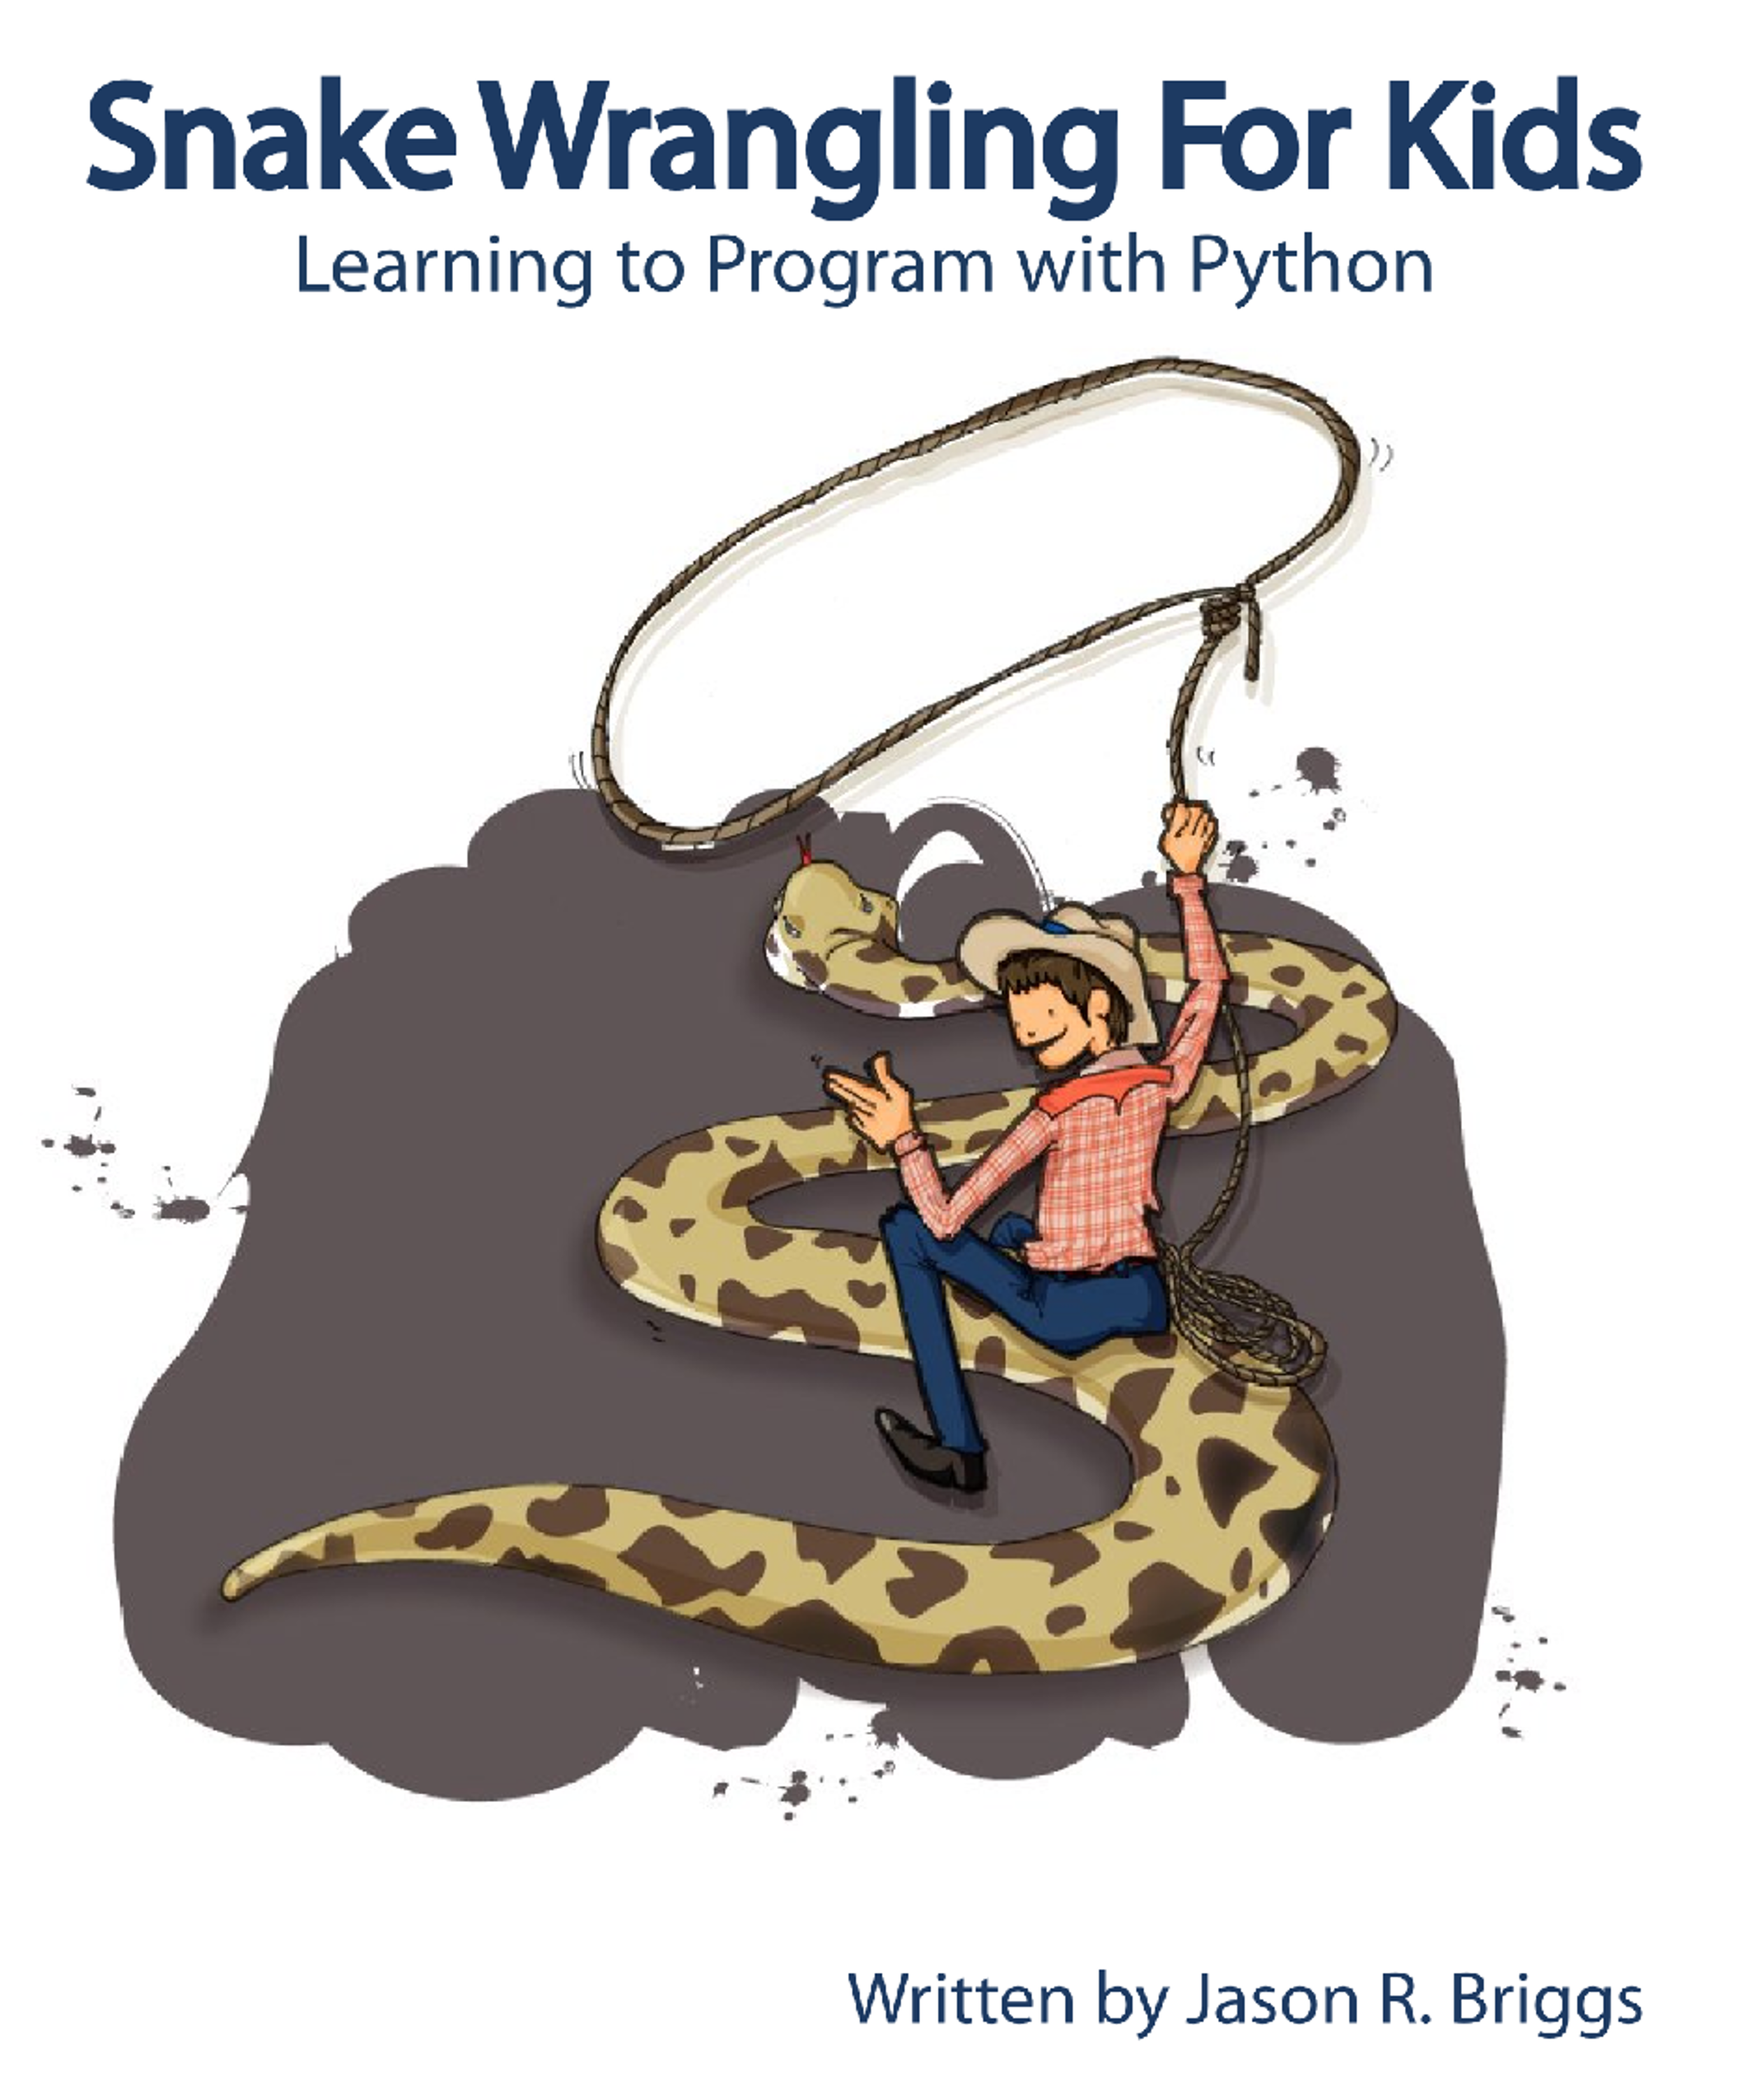
\includegraphics[width=0.9\paperwidth]{cover.eps}
\end{textblock*}
\begin{flushright}
\begin{WINDOWS}
\includegraphics[width=40mm]{windows-edition.eps} 
\end{WINDOWS}
\begin{MAC}
\includegraphics[width=40mm]{mac-edition.eps} 
\end{MAC}
\begin{LINUX}
\includegraphics[width=40mm]{linux-edition.eps} 
\end{LINUX}
\end{flushright}
\end{titlepage}
\end{FRONTCOVER}

\noindent
\textsf{\emph{Snake Wrangling for Kids, Learning to Program with Python}}\\
by Jason R. Briggs\\
\\
Version 0.7.7-python2.7
\\\\
Copyright \copyright 2007.\\
\\
Cover art and illustrations by Nuthapitol C.\\
\\
\noindent
\textsf{\emph{This book has been completely rewritten and updated, with new chapters (including developing graphical games), and new code examples. It also includes lots of fun programming puzzles to help cement the learning. Published by No Starch Press - available here: \href{http://nostarch.com/pythonforkids}{Python for Kids}. Also find more info \href{http://jasonrbriggs.com/python-for-kids/}{here}.}}
\\
\\
\linebreak
\noindent
Website:\\ \href{http://www.briggs.net.nz/log/writing/snake-wrangling-for-kids}{http://www.briggs.net.nz/log/writing/snake-wrangling-for-kids}\\ 
\\
\noindent
Thanks To:\\
Guido van Rossum (for benevelont dictatorship of the Python language), the members of the \href{http://www.python.org/community/sigs/current/edu-sig/}{Edu-Sig} mailing list (for helpful advice and commentary), author \href{http://www.davidbrin.com/}{David Brin} (the original \href{http://www.salon.com/tech/feature/2006/09/14/basic/}{instigator} of this book), Michel Weinachter (for providing better quality versions of the illustrations), and various people for providing feedback and errata, including: Paulo J. S. Silva, Tom Pohl, Janet Lathan, Martin Schimmels, and Mike Cariaso (among others).  Anyone left off this list, who shouldn't have been, is entirely due to premature senility on the part of the author.\\

\noindent
License:\\
\\
\includegraphics[width=40mm]{by-nc-sa.eps}\\
This work is licensed under the Creative Commons Attribution-Noncommercial-Share Alike 3.0 New Zealand License. To view a copy of this license, visit\\ \href{http://creativecommons.org/licenses/by-nc-sa/3.0/nz/}{http://creativecommons.org/licenses/by-nc-sa/3.0/nz/} or send a letter to Creative Commons, 171 Second Street, Suite 300, San Francisco, California, 94105, USA.\\

\noindent
Below is a summary of the license.\\

\noindent
You are free:
\begin{itemize}
 \item \textbf{to Share} — to copy, distribute and transmit the work 
 \item \textbf{to Remix} — to adapt the work
\end{itemize}
\noindent
Under the following conditions:
\begin{description}
 \item[Attribution.] You must attribute the work in the manner specified by the author or licensor (but not in any way that suggests that they endorse you or your use of the work).
 \item[Noncommercial.] You may not use this work for commercial purposes.
 \item[Share Alike.] If you alter, transform, or build upon this work, you may distribute the resulting work only under the same or similar license to this one.
\end{description}

\noindent
For any reuse or distribution, you must make clear to others the license terms of this work.\\

\noindent
Any of the above conditions can be waived if you get permission from the copyright holder.\\

\noindent
Nothing in this license impairs or restricts the author's moral rights.\\

\vspace*{4cm}
\begin{center}
\includegraphics[width=5cm]{python-powered.eps}
\end{center}

\mainmatter

\pagestyle{plain}

\pagenumbering{roman}
\tableofcontents


% preface.tex
% This work is licensed under the Creative Commons Attribution-Noncommercial-Share Alike 3.0 New Zealand License.
% To view a copy of this license, visit http://creativecommons.org/licenses/by-nc-sa/3.0/nz
% or send a letter to Creative Commons, 171 Second Street, Suite 300, San Francisco, California, 94105, USA.


\chapter*{Preface}\normalsize
    \addcontentsline{toc}{chapter}{Preface}
\begin{center}
{\em A Note to Parents...}
\end{center}
\pagestyle{plain}

\noindent
Dear Parental Unit or other Caregiver,

In order for your child to get started with programming, you're going to need to install Python (at least version 2.4 or greater) on your computer.
This is a fairly straight-forward task, but there are a few wrinkles depending upon what sort of Operating System you're using.  If you've just bought a shiny new computer, have no idea what to do with it, and that previous statement has filled you with a severe case of the cold chills, you'll probably want to find someone to do this for you.  Depending upon the state of your computer, and the speed of your internet connection, this could take anything from 15 minutes to a few hours.  See the instructions below for your specific platform...

\noindent
\emph{\color{BrickRed}Windows}

If you're using Windows, go to \href{http://www.python.org}{www.python.org} and download the latest Windows installer.  At time of writing, this is:
\begin{quote}
     \href{http://www.python.org/ftp/python/2.5/python-2.5.msi}{http://www.python.org/ftp/python/2.5/python-2.5.msi}
\end{quote}
Double-click the icon for the Windows installer (you do remember where you downloaded it to, don't you?), and then follow the instructions to install it in the default location (this is probably \emph{c:$\backslash$Python25}).

\noindent
\emph{\color{BrickRed}Mac OS X}

\noindent
If you're using Mac OS X, go to \href{www.pythonmac.org}{www.pythonmac.org} and download the Python package (as of Feb 2007, version 2.4.4).  If you're a Mac guru, you're probably already mumbling about the fact that Python is already installed on your system, or that Python 2.5 is available from python.org---both of which are true.  However, it's possible that neither the built-in version of Python nor version 2.5, downloadable from python.org, support Tkinter, which is a requirement for some of the examples in this book.  Save yourself the trouble and download the latest version of Python from this page:
\begin{quote}
    \href{http://pythonmac.org/packages/py24-fat/index.html}{http://pythonmac.org/packages/py24-fat/index.html}
\end{quote}
\noindent
Install by double-clicking on the .dmg file, and following the standard Mac install procedures.
If you still don't believe me, install the package you think should work, start up the Python console and try typing the following commands (one after the other) at the prompt: "import Tkinter" and "import turtle" (don't type the quotation marks).  If those commands succeed, then you were right and I was wrong.  I bow to your infinitesimally larger intelligence, Oh Great Mac Guru.

\noindent
\emph{\color{BrickRed}Linux}

\noindent
If you're a Linux user, download and install the latest version of Python (for example, 2.5) for your distribution.  Given the large number of Linux flavours, it's impossible to give exact details on installation for each---but chances are, if you're running Linux, you already know what you're doing anyway.  In fact, you're probably insulted by the very idea of being told how to install$\ldots$anything

\noindent
\emph{\color{BrickRed}After installation$\ldots$}

\noindent
$\ldots$You might need to sit down next to your child for the first few chapters, but hopefully after a few examples, they should be batting your hands away from the keyboard to do it themselves.  They should, at least, know how to use a text editor of some kind before they start (no, not a Word Processor, like Microsoft Word---a plain, old-fashioned text editor)---they should at least able to open and close files, create new text files and save what they're doing.  Apart from that, this book will try to teach the basics from there.
\\
\\
\noindent\\
Thanks for your time, and kind regards,
\noindent\\
THE BOOK

\pagestyle{headings}
\pagenumbering{arabic}

% ch1.tex
% This work is licensed under the Creative Commons Attribution-Noncommercial-Share Alike 3.0 New Zealand License.
% To view a copy of this license, visit http://creativecommons.org/licenses/by-nc-sa/3.0/nz
% or send a letter to Creative Commons, 171 Second Street, Suite 300, San Francisco, California, 94105, USA.


\chapter{Not all snakes will squish you}\label{ch:notallsnakeswillsquishyou}

Chances are you were given this book for your birthday.  Or possibly for Christmas.  Aunty Mildred was going to give you mismatching socks that were two sizes too large (and you wouldn't want to wear when you grew into them anyway).  Instead, she heard someone talking about this printable book, remembered you had one of those computer-thingamabobs that you tried to show her how to use last Christmas (you gave up when she started trying to talk into the mouse), and got them to print another copy.  Just be thankful you didn't get the mouldy old socks.

I hope you're not too disappointed that I popped out of the recycled wrapping paper, instead.  A not-quite-so-talkative (okay, not-talking-at-all) book, with an ominous looking title on the front about ``Learning$\ldots$''.
But take a moment to think about how I feel.  If you were the character from that novel about wizards that is sitting on the bookshelf in your bedroom, I'd possibly have teeth... or perhaps even eyes.  I might have moving pictures inside me, or be able to make moaning ghostly sounds when you opened my pages.  Instead, I'm printed out on dog-eared A4 sheets of paper, stapled together or perhaps bound in a folder.  How would I know---I don't have eyes.
\\
\\
\emph{I'd give anything for a nice, sharp set of teeth$\ldots$}
\\
\\
However it's not as bad as it sounds.  Even if I can't talk... or bite your fingers when you're not looking... I can tell you a little bit about what makes computers work.  Not the physical stuff, with wires and computer-chips and cables and devices that would, more than likely, electrocute you as soon as you touched them (so don't!!)---but the hidden stuff running around inside those wires and computer-chips and cables and bits, which make computers actually useful.

\begin{center}
\includegraphics*[width=70mm]{electrocute.eps}
\end{center}

It's a little like thoughts running around inside your head. If you didn't have thoughts you'd be sitting on the floor of your bedroom, staring vacantly at the door and drooling down the front of your t-shirt. Without \emph{programs}, computers would only be useful as a doorstop---and even then they wouldn't be very useful, because you'd keep tripping over them in the night.  And there's nothing worse than a stubbed toe in the dark.
\\
\\
\emph{I'm just a book and even I know that.}
\\
\\
Your family may have a Playstation, Xbox or Wii sitting in the lounge---they're not much use without programs (Games) to make them work.  Your DVD player, possibly your fridge and even your car, all have computer programs to make them more helpful than they would be otherwise.  Your DVD player has programs to help it figure out what to play on a DVD; your fridge might have a simple program to make sure it doesn't use too much electricity, but still keep your food cold; your car might have a computer with a program to warn the driver if they're about to bump into something.\\
If you know how to write computer programs, you can do all sorts of useful things. Perhaps write your own games. Create web pages that actually do stuff, instead of just sitting there looking somewhat colourful.  Being able to program could possibly even help with your homework.\\
\\
That said, let's get onto something a bit more interesting.

\section{A Few Words About Language}

Just like humans, certainly whales, possibly dolphins, and maybe even parents (although that's debatable), computers have their own language.  Actually, also like humans, they have more than one language.  There are languages covering just about all the letters of the alphabet.  A, B, C, D and E are not only letters, they're also programming languages (which proves that adults have no imagination, and should be made to read either a dictionary or a thesaurus before naming anything).

There are programming languages named after people, named using simple acronyms (the capital letters of a series of words), and just a few named after a TV show.  Oh, and if you add a few pluses and hashes (+, \#) after a couple of those letters I just listed---that's yet another couple of programming languages as well.  Making matters worse, some of the languages are almost the same, and differ only slightly.
\\
\\
\emph{What did I tell you?  No imagination!}
\\
\\
Luckily, many of these languages have fallen into disuse, or vanished completely; but the list of different ways you can `talk' to a computer is still rather worryingly large.  I'm only going to discuss one of them---otherwise we might as well not even get started.
\\
It would be more productive to sit in your bedroom and drool down the front of your t-shirt$\ldots$

\section{The Order of Non-venomous\\Constricting Serpentes$\ldots$}

$\ldots$or Pythons, for short.

Apart from being a snake, Python\index{Python} is also a programming language.  However, it was not named after a legless reptile; rather it is one of the few programming languages named after a TV show.  Monty Python was a British comedy show popular during the 1970's (and still popular now, actually), which you have to be a certain age to find amusing.  Anyone below the age of about$\ldots$ let's say 12$\ldots$ will wonder what all the fuss is all about\footnote{Except the fish slapping dance.  That's funny no matter how old you are.}.

There are a number of things about Python (the programming language, not the snake, nor the TV show) that make it extremely useful when you're learning to program.  For us, at the moment, the most important reason is that you can start it up and do stuff really quickly.

This is the part where you hope Mum, Dad (or whomever is in charge of the computer), has read the part at the beginning of this book labelled ``A Note for Mums and Dads''.

\noindent
There's a good way to find out if they actually have read it:

\subsection*{\color{BrickRed}If you're using Windows$\ldots$}\index{Windows}

Click on the Start button at the bottom left of the screen, click on `All Programs' (which has a green triangle next to it), and hopefully in the list of programs you should see `Python 2.5' (or something like it).  Figure~\ref{fig1} shows you what you should be looking for. Click on `Python (command line)' and you should see something like Figure~\ref{fig2}.

\begin{figure}
\begin{center}
\includegraphics[width=80mm]{figure1.eps}
\end{center}
\caption{Python in the Windows menu.}\label{fig1}
\end{figure}

\begin{figure}
\begin{center}
\includegraphics[width=135mm]{figure2.eps}
\end{center}
\caption{The Python console on Windows.}\label{fig2}
\end{figure}

\subsection*{\color{BrickRed}If you're using Mac OS X$\ldots$}\index{Mac OS X}

In Finder, on the left you should see a group called `Applications'.  Click on this, and then find a program called `Terminal' (it'll probably be in a folder called `Utilities').
Click on `Terminal', and when it starts up, type python and hit enter.  You'll should hopefully be looking at a window that looks like Figure~\ref{fig3}.

\begin{figure}
\begin{center}
\includegraphics[width=85mm]{figure3.eps}
\end{center}
\caption{The Python console on Mac OSX.}\label{fig3}
\end{figure}

\subsection*{\color{BrickRed}If you're using Linux$\ldots$}\index{Linux}

Ask Mum or Dad which terminal application you should use (it could be one called `Konsole', `rxvt', `xterm' or any one of a dozen different programs---which is why you'll probably need to ask).  Start the terminal program and type `python' (without the quotes), and hit enter.  You should see something like Figure~\ref{fig4}.

\begin{figure}
\begin{center}
\includegraphics[width=80mm]{figure4.eps}
\end{center}
\caption{The Python console on Linux.}\label{fig4}
\end{figure}

\subsection*{\color{BrickRed}If you discover they haven't read the section in the beginning$\ldots$}

$\ldots$because you can't find any of those programs---then turn to the front of the book, poke it under their nose while they're trying to read the newspaper, and look hopeful.  Saying, ``please please please please'' over and over again, until it becomes annoying, might work quite well, if you're having trouble convincing them to get off the couch.

\section{Your first Python program}

With any luck, if you've reached this point, you've managed to start up the Python console, which is one way of running Python commands and programs.  When you first start the console (or after entering a command), you'll see what's called a `prompt'.  In the Python console\index{Python console}, the prompt is three chevrons, or greater-than symbols ($>$) pointing to the right:

\begin{listing}
\begin{verbatim}
>>>
\end{verbatim}
\end{listing}

If you put enough Python commands together, you have a program that you can run in more than just the console$\ldots$ but for the moment we're going to keep things simple, and type our commands directly in the console, at the prompt ($>>>$).  So, why not start with typing the following:

\begin{listing}
\begin{verbatim}
print "Hello World"
\end{verbatim}
\end{listing}

Make sure you include the quotes (that's these: $"$ $"$), and hit enter at the end of the line.  Hopefully you'll see something like the following:

\begin{listing}
\begin{verbatim}
>>> print "Hello World"
Hello World
\end{verbatim}
\end{listing}

The prompt reappears, to let you know that the Python console is ready to accept more commands.

\noindent
Congratulations! You've just created your first Python program.

\section{Your Second Python program$\ldots$the same again?}

Python programs wouldn't be all that useful if you had to type the commands every single time you wanted to do something---or if you wrote a program for someone, and they had to type it in before they could use it.

The Word Processor that you might be using to write your school assignments, is probably somewhere between 10 and 100 million lines of code.  Depending upon how many lines you printed on one page (and whether or not you printed on both sides of the paper), this could be around 400,000 printed pages$\ldots$ or a stack of paper about 40 metres high.
Just imagine when you brought that software home from the shop, there would be quite a few trips back and forth to the car, to carry that much paper$\ldots$

$\ldots$and you'd better hope there's no big gust of wind while you're carrying those stacks. Luckily, there's an alternative to all this typing---or no one would get anything done.

\begin{center}
\includegraphics*[width=85mm]{pullinghair.eps}
\end{center}

\subsection*{\color{BrickRed}If you're using Windows$\ldots$}\index{Windows}

Open Notepad (Click on Start, All Programs, and it should be in the Accessories sub menu), and then type the print command exactly as you typed it into the console before:

\begin{listing}
\begin{verbatim}
print "Hello World"
\end{verbatim}
\end{listing}

Click on the File menu (in Notepad), then Save, and when prompted for a file name, call it \emph{hello.py} and save it on your Desktop. Double-click on the icon for hello.py on your Desktop (see Figure~\ref{fig5}) and for a brief moment a console window will appear.  It will vanish too quickly for you too make out the words, but Hello World will have been printed to the screen for a fraction of a second---we'll come back to this later and prove that it did.\\

\begin{figure}
\begin{center}
\includegraphics[width=58mm]{figure5.eps}
\end{center}
\caption{hello.py icon on the Windows Desktop.}\label{fig5}
\end{figure}

\subsection*{\color{BrickRed}If you're using Mac OS X$\ldots$}\index{Mac OS X}

Open up the Text Editor by clicking on its icon.  It may be in the Dock at the bottom of the screen \includegraphics*[width=12mm]{textedit-icon.eps}, or look for this icon \includegraphics*[width=19mm]{textedit-icon2.eps} in the Applications list in Finder.  Type the print command exactly as you typed it into the console earlier:

\begin{listing}
\begin{verbatim}
print "Hello World"
\end{verbatim}
\end{listing}

Click on the File menu, then click on Save, and when you are prompted for a file name, call it hello.py and save it on your Desktop. If you double-click on hello.py on your Desktop, you'll probably get some odd dialog boxes popping up with rather cryptic messages.  The first dialog might look like Figure~\ref{fig6}.

\begin{figure}
\begin{center}
\includegraphics[width=99mm]{figure6.eps}
\end{center}
\caption{The first odd dialog box.}\label{fig6}
\end{figure}

Click the Open button.  You might need to double-click on the hello.py icon again.  In which case you'll get a slightly different dialog (see Figure~\ref{fig7}).

\begin{figure}
\begin{center}
\includegraphics[width=99mm]{figure7.eps}
\end{center}
\caption{The second odd dialog box.}\label{fig7}
\end{figure}

At which point, the `Terminal' application will automatically start, followed by a second window that might look something like Figure~\ref{fig8}.

\begin{figure}
\begin{center}
\includegraphics[width=119mm]{figure8.eps}
\end{center}
\caption{The final window.}\label{fig8}
\end{figure}

\emph{What a mess!}

But you can see that the words Hello World were printed in that last window (the fourth line from the bottom of the text).

\subsection*{\color{BrickRed}If you're using Linux$\ldots$}\index{Linux}

Open a text editor (again you might have to ask Mum or Dad which one to use), then type the print command exactly as you typed it into the console:

\begin{listing}
\begin{verbatim}
print "Hello World"
\end{verbatim}
\end{listing}

Click on the File menu, then Save, and when prompted for a file name, call it hello.py and save it in your Home folder (there might be an icon called `Home' somewhere in the Save dialog box).  Next open up the terminal application (again Konsole, rxvt, etc... what we used earlier), and type:

\begin{listing}
\begin{verbatim}
python hello.py
\end{verbatim}
\end{listing}

You should see Hello World written to the window exactly as it was when you typed the command in the Python console (see Figure~\ref{fig9}).

\begin{figure}
\begin{center}
\includegraphics[width=75mm]{figure9.eps}
\end{center}
\caption{Running a python program from a text file on Linux.}\label{fig9}
\end{figure}

\subsection*{\color{BrickRed}Continuing here$\ldots$}

And so, you can now see that the nice people who created Python, have kindly saved you from having to type the same thing over and over and over and over and over again.  Like they did back in the 1980's.  No, I'm serious---they did.  Go and ask your Dad if he ever owned a ZX81 when he was younger?\\

\noindent
If he did you can point at him and laugh.\\

\noindent
Trust me on this one.  You won't get it.  But he will.\footnote{The Sinclair ZX81, released in the 1980's was one of the first affordable home computers.  A number of young boys and girls were driven completely mad, typing in the code for games printed in popular ZX81 magazines---only to discover, after hours of typing, that the darn things never worked properly.}

\noindent
\emph{Be prepared to run away though.}

\subsection*{\color{BrickRed}$\ldots$Only to end here}

Welcome to the wonderful world of Programming.  We've started really simply with a ``Hello World'' application---everyone starts with that, when they're learning to program.
In the next chapter we'll start to do some more useful things with the Python console and then look at what goes into making a program.

\newpage
% ch2.tex
% This work is licensed under the Creative Commons Attribution-Noncommercial-Share Alike 3.0 New Zealand License.
% To view a copy of this license, visit http://creativecommons.org/licenses/by-nc-sa/3.0/nz
% or send a letter to Creative Commons, 171 Second Street, Suite 300, San Francisco, California, 94105, USA.


\chapter{8 multiplied by 3.57 equals$\ldots$}\label{ch:8multipliedby3.57}

What is 8 multiplied by 3.57?  You'd have to use a calculator, wouldn't you?  Well perhaps you're extremely smart and can do multiplication of fractions in your head---but that's not the point.  You can also do the same thing with the Python console. Start up the console again (see Chapter~\ref{ch:notallsnakeswillsquishyou} for more information, if you've skipped ahead for some strange reason), and once you see the prompt, type 8$*$3.57 and press the Enter key:

\begin{listing}
\begin{verbatim}
Python 3.0 (r30:67503, Dec  6 2008, 23:22:48) 
Type "help", "copyright", "credits" or "license" for more information.
>>> 8 * 3.57
28.559999999999999
\end{verbatim}
\end{listing}

The star (*), or asterisk key (shift 8 on some keyboards), is used for multiplication\index{multiplication}, instead of the normal times symbol (\textsf{X}) that you use at school (using the star key is necessary, otherwise how would the computer know whether you meant the letter \emph{x} or the multiplication symbol \textsf{X} ?).  How about an equation that's a bit more useful?

Suppose you do chores once a week, for which you get \$5 pocket money, and you have a paper round which you do 5 times a week and get \$30---how much money would you earn in a year?

\begin{figure}[t]
\begin{center}
\fbox{\colorbox{PaleBlue}{\parbox{.75\linewidth} {
\subsection*{Python is broken!?!?}

If you just picked up a calculator and entered 8 x 3.57 the answer showing on the display will be:\\

\textsf{
28.56\\
}

\noindent
Why is Python different?  Is it broken?\\

\noindent
Actually, no. The reason can be found in the way floating point\index{floating point} (fractional numbers with a decimal place) numbers are handled by the computer.  It's a complicated and somewhat confusing problem for beginners, so it's best to just remember that when you're working with fractions (i.e. with a decimal place on a number), \emph{sometimes} the result won't be exactly what you were expecting. This is true for multiplication, division, addition or subtraction.
}}}
\end{center}
\end{figure}

If we were writing that on paper, we might write something like:
\begin{verbatim}
(5 + 30) x 52
\end{verbatim}

Which is \$5 + \$30 multiplied by 52 weeks in a year.  \begin{samepage}Of course, we're smart, and we know that 5 + 30 is 35, so the equation is really:

\begin{verbatim}
35 x 52
\end{verbatim}
\end{samepage}

Which is easy enough to do in a calculator, or on paper.  But we can do all of these calculations with the console as well:

\begin{listing}
\begin{verbatim}
>>> (5 + 30) * 52
1820
>>> 35 * 52
1820
\end{verbatim}
\end{listing}

So, what if you spend \$10 each week?  How much do you have left at the end of the year?  We could write the equation on paper a couple of different ways, but let's just type it into the console:

\begin{listing}
\begin{verbatim}
>>> (5 + 30 - 10) * 52
1300
\end{verbatim}
\end{listing}

That's \$5 and \$30 minus \$10 multiplied by 52 weeks in the year.  And you'd have \$1300 left at the end of the year. Okay, so that's not looking all that useful so far.  We can do all of that with a calculator.  But we'll come back to this later and show how to make it much more useful.

You can do multiplication\index{multiplication} and addition\index{addition} (obviously), and subtraction\index{subtraction} and division\index{division} in the Python console, along with a bunch of other maths operations that we won't go into now.  For the moment the basic maths symbols for Python (actually they're called operators\index{operators}) are:

\begin{center}
\begin{tabular}{|c|c|}
\hline
+ & Addition \\
\hline
- & Subtraction \\
\hline
* & Multiplication \\
\hline
/ & Division \\
\hline
\end{tabular}
\end{center}

The reason the forward-slash (/) is used for division, is that it would be rather difficult to draw a division line (plus they didn't bother to put a division symbol $\div$ on the computer keyboard) as you're supposed to use for written equations.  For example if you had 100 eggs and 20 boxes, you might want to know how many eggs would go in each box, so you'd show dividing 100 into 20, by writing the following equation:

\begin{displaymath}
\frac{100}{20}
\end{displaymath}

Or if you know about long division, you might write it out fully like this:

\begin{displaymath}
\longdiv{100}{20}
\end{displaymath}

Or you might even write it like this:

\begin{displaymath}
100 \div 20
\end{displaymath}

However, in Python terms you would just type it as ``100 / 20''.

\emph{Which is much easier, I think.  But then, I'm a book---what do I know?}

\section{Use of brackets and ``Order of Operations''}\index{order of operations}

We use brackets in a programming language to control what is called ``Order of Operations''.  An operation is the use of an operator (one of those symbols in the table above).  There are more operators than those basic symbols, but for that simple list (addition, subtraction, multiplication and division), it's enough to know that multiplication and division both have a higher order than addition and subtraction.  Which means you do the multiplication or division part of an equation before you do the addition or subtraction part.  In the following equation, all the operators are addition (+), the numbers are added in order:

\begin{listing}
\begin{verbatim}
>>> print(5 + 30 + 20)
55
\end{verbatim}
\end{listing}

\noindent
Similarly, in this equation, there are only addition and subtraction operators, so again Python considers each number in the order it appears:

\begin{listing}
\begin{verbatim}
>>> print(5 + 30 - 20)
15
\end{verbatim}
\end{listing}

\noindent
But in the following equation, there is a multiplication operator, so the numbers 30 and 20 are considered first.  The equation is another way of saying, ``multiply 30 by 20, then add 5 to the result'' (multiplication first, because it has a higher order than addition):

\begin{listing}
\begin{verbatim}
>>> print(5 + 30 * 20)
605
\end{verbatim}
\end{listing}

\noindent
So what happens when we add brackets?  The following equation shows the result:

\begin{listing}
\begin{verbatim}
>>> print((5 + 30) * 20)
700
\end{verbatim}
\end{listing}

\noindent
Why is the number different?  Because brackets control the order of operations.  With brackets, Python knows to calculate using the operators in the brackets first, then do the operators outside.  So that equation is another way of saying, ``add 5 and 30, then multiply the result by 20''.
The use of brackets can become more complicated.  There can be brackets inside brackets:

\begin{listing}
\begin{verbatim}
>>> print(((5 + 30) * 20) / 10)
70
\end{verbatim}
\end{listing}

\noindent
In this case, Python evaluates the \textbf{inner} most brackets first, then the outer brackets, and then the other operator.  So this equation is a way of saying, ``add 5 and 30, then multiply the result by 20, finally divide that result by 10''.  The result without brackets is again slightly different:

\begin{listing}
\begin{verbatim}
>>> 5 + 30 * 20 / 10
65
\end{verbatim}
\end{listing}

In this case 30 is multiplied by 20 first, then the result is divided by 10, finally 5 is added to the final result.

\emph{Remember that multiplication and division always go before addition and subtraction, unless brackets are used to control the order of operations.}

\section{There's nothing so fickle as a variable}\index{variable}

A `variable' is a programming term used to describe a place to store things.  The `things' can be numbers, or text, or lists of numbers and text---and all sorts of other items too numerous to go into here.  For the moment, let's just think of a variable as something a bit like a mailbox.

\begin{center}
\includegraphics*[width=76mm]{girlbubble.eps}
\end{center}

You can put things (such as a letter or a package) in a mailbox, just as you can put things (numbers, text, lists of numbers and text, etc, etc, etc) in a variable.  This mailbox idea is the way many programming languages work.  But not all.

In Python, variables are slightly different.  Rather than being a mailbox with things in it, a variable is more like a label which is stuck on the outside of the mailbox.  We can pull that label off and stick it on something else, or even tie the label (perhaps with a piece of string) to more than one thing. We create a variable by giving it a name, using an equals sign (=), then telling Python what we want that name to point to.  For example:

\begin{listing}
\begin{verbatim}
>>> fred = 100
\end{verbatim}
\end{listing}

We've just created a variable called `fred' and said that it points to the number 100.  It's a bit like telling Python to remember that number because we want to use it later.  To find out what a variable is pointing at, we can just type `print' in the console, followed by the variable name, and hit the Enter key.  For example:

\begin{listing}
\begin{verbatim}
>>> fred = 100
>>> print(fred)
100
\end{verbatim}
\end{listing}

We can also tell Python we want the variable \code{fred} to point at something else:

\begin{listing}
\begin{verbatim}
>>> fred = 200
>>> print(fred)
200
\end{verbatim}
\end{listing}

\noindent
On the first line we say we now want fred to point at the number 200.  Then, in the second line, we ask what fred is pointing at just to prove it changed. We can also point more than one name at the same item:

\begin{listing}
\begin{verbatim}
>>> fred = 200
>>> john = fred
>>> print(john)
200
\end{verbatim}
\end{listing}

In the code above, we're saying that we want the name (or label) \code{john} to point at the same thing \code{fred} is pointing to.
Of course, `fred' isn't a very useful name for a variable.  It doesn't tell us anything about what it's used for.  A mailbox is easy---you use a mailbox for mail.  But a variable can have a number of different uses, and can point at a whole bunch of different things, so we usually want something more informative as its name.
\par
Suppose you started up the Python console, typed `fred = 200', then went away---spent 10 years climbing Mount Everest, crossing the Sahara desert, bungy-jumping off a bridge in New Zealand, and finally, sailing down the Amazon river---when you came back to your computer, would you remember what that number 200 meant (and what it was for)?

\noindent
\emph{I don't think I would.}

\noindent
I just made it up now, and I have no idea what `fred = 200' means (other than a \emph{name} pointing at the number \emph{200}).  So after 10 years, you'll have absolutely no chance of remembering.
\par
Aha!  But, what if we called our variable: \emph{number\_of\_students}.

\begin{listing}
\begin{verbatim}
>>> number_of_students = 200
\end{verbatim}
\end{listing}

We can do that because variable names can be made up of letters, numbers and (\_) underscores---although they cannot start with a number.  If you come back after 10 years, `number\_of\_students' still makes sense.  You can type:

\begin{listing}
\begin{verbatim}
>>> print(number_of_students)
200
\end{verbatim}
\end{listing}

\noindent
And you'll immediately know that we're talking about 200 students.  It's not always important to come up with meaningful names for variables.  You can use anything from single letters (such as `a') to large sentences; and sometimes, if you're doing something quick, a simple and short variable name is just as useful.  It depends very much upon whether you want to be able to look at that variable name later and figure out what on earth you were thinking at the time you typed it in.

\begin{listing}
\begin{verbatim}
this_is_also_a_valid_variable_name_but_perhaps_not_very_useful
\end{verbatim}
\end{listing}

\section{Using Variable}\index{Variables}

Now we know how to create a variable, how do we use it?  Remember that equation we came up with earlier?  The one to work out how much money you'd have left at the end of the year, if you earned \$5 a week doing chores, \$30 a week on a paper round, and spent \$10 per week.  So far we have:

\begin{listing}
\begin{verbatim}
>>> print((5 + 30 - 10) * 52)
1300
\end{verbatim}
\end{listing}

\noindent
What if we turn the first 3 numbers into variables?  Try typing the following:

\begin{listing}
\begin{verbatim}
>>> chores = 5
>>> paper_round = 30
>>> spending = 10
\end{verbatim}
\end{listing}

\noindent
We've just created variables named `chores', `paper\_round' and `spending'.  We can then re-type the equation to get:

\begin{listing}
\begin{verbatim}
>>> print((chores + paper_round - spending) * 52)
1300
\end{verbatim}
\end{listing}

Which gives the exact same answer.  What if you get \$2 more per week, for doing extra chores.  Change the `chores' variable to 7, then hit the up-arrow key ($\uparrow$) on your keyboard a couple of times, until the equation re-appears, and hit the Enter key:

\begin{listing}
\begin{verbatim}
>>> chores = 7
>>> print((chores + paper_round - spending) * 52)
1404
\end{verbatim}
\end{listing}

That's a lot less typing to find out that you now end up with \$1404 at the end of the year.  You can try changing the other variables, then hit the up-arrow to perform the calculation again, and see what effect it has.

\begin{listing}
\begin{verbatim}
If you spend twice as much money per week:
>>> spending = 20
>>> print((chores + paper_round - spending) * 52)
884
\end{verbatim}
\end{listing}

You're only left with \$884 savings at the end of the year. This is still only slightly useful.  We haven't hit really useful yet.  But for the moment, it's enough to understand that variables are used to store things.

\noindent
\emph{Think of a mailbox with a label on it!}

\section{A Piece of String?}\index{strings}

If you're paying attention, and not just skimming through looking for the good bits, you might remember I mentioned that variables can be used for all sorts of things---not just numbers. In programming, most of the time we call text a `string'. Which might seem a bit weird; but if you think that text is just `stringing together' (or joining together) a bunch of letters, perhaps it might make a little more sense.

\noindent
\emph{Then again, perhaps it doesn't.}

In which case, all you need to know, is that a string is just a bunch of letters and numbers and other symbols put together in some meaningful way. All the letters, and numbers, and symbols in this book could make up a string.  Your name could be a string.  So could your home address.  The first Python program we created in Chapter \ref{ch:notallsnakeswillsquishyou}, used a string: `Hello World'.
\par
In Python, we create a string by putting quotes around the text.  So we can take our useless \code{fred} variable, and put a string inside it like this:

\begin{listing}
\begin{verbatim}
>>> fred = "this is a string"
\end{verbatim}
\end{listing}

\noindent
And we can see what's inside the \code{fred} variable, by typing \code{print(fred)}:

\begin{listing}
\begin{verbatim}
>>> print(fred)
this is a string
\end{verbatim}
\end{listing}

\noindent
We can also use single-quotes to create a string:

\begin{listing}
\begin{verbatim}
>>> fred = 'this is yet another string'
>>> print(fred)
this is yet another string
\end{verbatim}
\end{listing}

However, if you try to type more than one line of text for your string using a single quote (') or double quote ("), you'll get an error message in the console. For example, type the following line and hit Enter, and you'll get a fairly scary error message similar to the following:

\begin{listing}
\begin{verbatim}
>>> fred = "this is two
  File "<stdin>", line 1
    fred = "this is two
                      ^
SyntaxError: EOL while scanning string literal
\end{verbatim}
\end{listing}

\index{multi-line string}We'll talk more about errors later, but for the moment, if you want more than one line of text, you can use 3 single quotes:

\begin{listing}
\begin{verbatim}
>>> fred = '''this is two
... lines of text in a single string'''
\end{verbatim}
\end{listing}

\noindent
Print out the contents to see if it worked:

\begin{listing}
\begin{verbatim}
>>> print(fred)
this is two
lines of text in a single string
\end{verbatim}
\end{listing}

By the way, you'll see those 3 dots (...) quite a few times when you're typing something that continues onto another line (like a multi line string).  In fact, you'll see it a lot more as we continue.

\section{Tricks with Strings}\label{trickswithstrings}

Here's an interesting question:  what's 10 * 5 (10 times 5)?  The answer is, of course, 50.

\noindent
\emph{All right, that's not an interesting question at all.}

But what is 10 * 'a' (10 times the letter a)?  It might seem like a nonsensical question, but here's the answer from the World of Python:

\begin{listing}
\begin{verbatim}
>>> print(10 * 'a')
aaaaaaaaaa
\end{verbatim}
\end{listing}

This works with more than just single character strings:

\begin{listing}
\begin{verbatim}
>>> print(20 * 'abcd')
abcdabcdabcdabcdabcdabcdabcdabcdabcdabcdabcdabcdabcdabcdabcdabcdabcdabcdabcdabcd
\end{verbatim}
\end{listing}

Another trick with a string, is embedding values.  You can do this by using \%s, which is like a marker (or a placeholder) for a value you want to include in a string.  It's easier to explain with an example:

\begin{listing}
\begin{verbatim}
>>> mytext = 'I am %s years old'
>>> print(mytext % 12)
I am 12 years old
\end{verbatim}
\end{listing}

In the first line, the variable mytext is created with a string containing some words and a placeholder (\%s).  The \%s is a little beacon saying ``replace me with something'' to the Python console.  So on the next line, when we call \code{print(mytext)}, we use the \% symbol, to tell Python to replace the marker with the number 12. We can reuse that string and pass in different values:

\begin{listing}
\begin{verbatim}
>>> mytext = 'Hello %s, how are you today?'
>>> name1 = 'Joe'
>>> name2 = 'Jane'
>>> print(mytext % name1)
Hello Joe, how are you today?
>>> print(mytext % name2)
Hello Jane, how are you today?
\end{verbatim}
\end{listing}

In the above example, 3 variables (mytext, name1 and name2) are created---the first includes the string with the marker.  Then we can print the variable `mytext', and again use the \% operator to pass in variables `name1' and `name2'.  You can use more than one placeholder:

\begin{listing}
\begin{verbatim}
>>> mytext = 'Hello %s and %s, how are you today?'
>>> print(mytext % (name1, name2))
Hello Joe and Jane, how are you today?
\end{verbatim}
\end{listing}

When using more than one marker, you need to wrap the replacement values with brackets---so (name1, name2) is the proper way to pass 2 variables. A set of values surrounded by brackets (the round ones, not the square ones) is called a \emph{tuple}, and is a little bit like a list, which we'll talk about next.

\section{Not quite a shopping list}\index{lists}

Eggs, milk, cheese, celery, peanut butter, and baking soda.  Which is not quite a full shopping list, but good enough for our purposes. If you wanted to store this in a variable you could create a string:

\begin{listing}
\begin{verbatim}
>>> shopping_list = 'eggs, milk, cheese, celery, peanut butter, baking soda'
>>> print(shopping_list)
eggs, milk, cheese, celery, peanut butter, baking soda
\end{verbatim}
\end{listing}

Another way would be to create a `list', which is a special kind of object in Python:

\begin{listing}
\begin{verbatim}
>>> shopping_list = [ 'eggs', 'milk', 'cheese', 'celery', 'peanut butter', 
... 'baking soda' ]
>>> print(shopping_list)
['eggs', 'milk', 'cheese', 'celery', 'peanut butter', 'baking soda']
\end{verbatim}
\end{listing}

This is more typing, but it's also more useful.  We could print the 3rd item in the list by using its position (called its index position), inside square brackets []:

\begin{listing}
\begin{verbatim}
>>> print(shopping_list[2])
cheese
\end{verbatim}
\end{listing}

Lists start at index position 0---so the first item in a list is 0, the second is 1, the third is 2.  That doesn't make a lot of sense to most people, but it does to programmers.  Pretty soon, when you walk up some stairs you'll start counting with zero rather than one.  That will really confuse your little brother or sister.
\par
We can show all the items from the 3rd item up to the 5th in the list, by using a colon inside the square brackets:

\begin{listing}
\begin{verbatim}
>>> print(shopping_list[2:5])
['cheese', 'celery', 'peanut butter']
\end{verbatim}
\end{listing}

[2:5] is the same as saying that we are interested in items from index position 2 up to (but not including) index position 5.  And, of course, because we start counting with 0, the 3rd item in the list is actually number 2, and the 5th item is actually number 4. Lists can be used to store all sorts of items.  They can store numbers:

\begin{listing}
\begin{verbatim}
>>> mylist = [ 1, 2, 5, 10, 20 ]
\end{verbatim}
\end{listing}

\noindent
And strings:

\begin{listing}
\begin{verbatim}
>>> mylist = [ 'a', 'bbb', 'ccccccc', 'ddddddddd' ]
\end{verbatim}
\end{listing}

\noindent
And mixtures of numbers and strings:

\begin{listing}
\begin{verbatim}
>>> mylist = [1, 2, 'a', 'bbb']
>>> print(mylist)
[1, 2, 'a', 'bbb']
\end{verbatim}
\end{listing}

\noindent
And even lists of lists:

\begin{listing}
\begin{verbatim}
>>> list1 = [ 'a', 'b', 'c' ]
>>> list2 = [ 1, 2, 3 ]
>>> mylist = [ list1, list2 ]
>>> print(mylist)
[['a', 'b', 'c'], [1, 2, 3]]
\end{verbatim}
\end{listing}

In the above example, a variable called `list1' is created with 3 letters, `list2' is created with a 3 numbers, and `mylist' is created using list1 and list2. Things can get rather confusing, rather quickly, if you start creating lists of lists of lists of lists$\ldots$ but luckily there's not usually much need for making things that complicated in Python. Still it is handy to know that you can store all sorts of items in a Python list.

\noindent
\emph{And not just your shopping.}

\subsection*{\color{BrickRed}Replacing items}\index{lists!replacing}

We can replace an item in the list, by setting its value in a similar way to setting the value of a normal variable. For example, we could change celery to lettuce by setting the value in index position 3:

\begin{listing}
\begin{verbatim}
>>> shopping_list[3] = 'lettuce'
>>> print(shopping_list)
['eggs', 'milk', 'cheese', 'lettuce', 'peanut butter', 'baking soda']
\end{verbatim}
\end{listing}

\subsection*{\color{BrickRed}Adding more items...}\index{lists!appending}

We can add items to a list by using a method called `append'.  A method is an action or command that tells Python that we want to do something.  We'll talk more about methods later, but for the moment, to add an item to our shopping list, we can do the following:

\begin{listing}
\begin{verbatim}
>>> shopping_list.append('chocolate bar')
>>> print(shopping_list)
['eggs', 'milk', 'cheese', 'lettuce', 'peanut butter', 'baking soda', 
'chocolate bar']
\end{verbatim}
\end{listing}

Which, if nothing else, is certainly an improved shopping list.

\subsection*{\color{BrickRed}$\ldots$and removing items}\index{lists!removing}

We can remove items from a list by using the command `del' (short for delete).  For example, to remove the 6th item in the list (baking soda):

\begin{listing}
\begin{verbatim}
>>> del shopping_list[5]
>>> print(shopping_list)
['eggs', 'milk', 'cheese', 'lettuce', 'peanut butter', 'chocolate bar']
\end{verbatim}
\end{listing}

Remember that positions start at zero, so shopping\_list[5] actually refers to the 6th item.

\subsection*{\color{BrickRed}2 lists are better than 1}\index{lists!joining}

We can join lists together by adding them, as if we were adding two numbers:

\begin{listing}
\begin{verbatim}
>>> list1 = [ 1, 2, 3 ]
>>> list2 = [ 4, 5, 6 ]
>>> print(list1 + list2)
[1, 2, 3, 4, 5, 6]
\end{verbatim}
\end{listing}

\noindent
We can also add the two lists and set the result to another variable:

\begin{listing}
\begin{verbatim}
>>> list1 = [ 1, 2, 3 ]
>>> list2 = [ 4, 5, 6 ]
>>> list3 = list1 + list2
>>> print(list3)
[1, 2, 3, 4, 5, 6]
\end{verbatim}
\end{listing}

\noindent
And you can multiply a list in the same way we multiplied a string:

\begin{listing}
\begin{verbatim}
>>> list1 = [ 1, 2 ]
>>> print(list1 * 5)
[1, 2, 1, 2, 1, 2, 1, 2, 1, 2]
\end{verbatim}
\end{listing}

\noindent
In the above example, multiplying list1 by five is another way of saying ``repeat list1 five times''. However, division (/) and subtraction (-) don't make sense when working with lists, so you'll get errors when trying the following examples:

\begin{listing}
\begin{verbatim}
>>> list1 / 20
Traceback (most recent call last):
  File "<stdin>", line 1, in <module>
TypeError: unsupported operand type(s) for /: 'list' and 'int'
\end{verbatim}
\end{listing}

\noindent
or:

\begin{listing}
\begin{verbatim}
>>> list1 - 20
Traceback (most recent call last):
  File "<stdin>", line 1, in <module>
TypeError: unsupported operand type(s) for -: 'type' and 'int'
\end{verbatim}
\end{listing}

\noindent
You'll get a rather nasty error message.

\section{Tuples and Lists}\label{tuplesandlists}\index{tuples}

A tuple (mentioned earlier) is a little bit like a list, but rather than using square brackets, you use round brackets---e.g. `(' and `)'.  You can use tuples in a similar way to a list:

\begin{listing}
\begin{verbatim}
>>> t = (1, 2, 3)
>>> print(t[1])
2
\end{verbatim}
\end{listing}

The main difference is that, unlike lists, tuples can't change, once you've created them.  So if you try to replace a value like we did earlier with the list, you'll get another error message:

\begin{listing}
\begin{verbatim}
>>> t[0] = 4
Traceback (most recent call last):
  File "<stdin>", line 1, in ?
TypeError: 'tuple' object does not support item assignment
\end{verbatim}
\end{listing}

That doesn't mean you can't change the variable containing the tuple to something else.  For example, this code will work fine:

\begin{listing}
\begin{verbatim}
>>> myvar = (1, 2, 3)
>>> myvar = [ 'a', 'list', 'of', 'strings' ]
\end{verbatim}
\end{listing}

First we create the variable \code{myvar} pointing to a tuple of 3 numbers.  Then we change \code{myvar} to point at a list of strings. This might be a bit confusing at first.  But think of it like lockers in a school.  Each locker has a name tag on it. You put something in the locker, close the door, lock it, then throw away the key.  You then peel the name tag off, wander over to another empty locker, and stick something else in that (but this time you keep the key).  A tuple is like the locked locker.  You can't change what's inside it.  But you can take the label off and stick it on an unlocked locker, and then put stuff inside that locker and take stuff out---that's the list.

\section{Things to try}

\emph{In this chapter we saw how to calculate simple mathematical equations using the Python console.  We also saw how brackets can change the result of an equation, by controlling the order that operators are used.  We found out how to tell Python to remember values for later use---using variables---plus how Python uses `strings' for storing text, and lists and tuples, for handling more than one item.}
\par

\subsection*{Exercise 1}
Make a list of your favourite toys and name it \code{toys}.  Make a list of your favourite foods and name it \code{foods}.  Join these two lists and name the result \code{favourites}.  Finally print the variable \code{favourites}.

\subsection*{Exercise 2}
If you have 3 boxes containing 25 chocolates, and 10 bags containing 32 sweets, how many sweets and chocolates do you have in total?  (Note: you can do this with one equation with the Python console)

\subsection*{Exercise 3}
Create variables for your first and last name. Now create a string and use placeholders to add your name.


\newpage
% ch3.tex
% This work is licensed under the Creative Commons Attribution-Noncommercial-Share Alike 3.0 New Zealand License.
% To view a copy of this license, visit http://creativecommons.org/licenses/by-nc-sa/3.0/nz
% or send a letter to Creative Commons, 171 Second Street, Suite 300, San Francisco, California, 94105, USA.


\chapter{Turtles, and other slow moving creatures}\index{turtle}\label{ch:turtles}

There are certain similarities between turtles in the real world and a Python turtle.  In the real world, a turtle is a (sometimes) green reptile that moves around very slowly and carries its house on its back.  In the world of Python, a turtle is a small black arrow that moves very slowly around the screen. No mention of house-carrying though.

In fact, considering that a Python turtle leaves a trail as it moves around the screen, this makes it less like a real turtle, and more like a snail or a slug.  However, I suppose that a module called `slug' wouldn't be particularly attractive, so it makes sense to stick with turtles.  Just imagine the turtle is carrying a couple of marker pens with it, and drawing as it goes.

In the deep, dark, and distant past, there was a simple programming language called Logo.  Logo was used to control a robot turtle (called Irving).  Over time, the turtle evolved from a robot that could move around the floor, to a small arrow moving around a screen.

\emph{Which just goes to show, things don't always improve as technology advances---a little robot turtle would be a lot more fun.}

Python's turtle module (we'll come to modules a bit later, but for now just just think of a module as something we can use inside a program) is a little bit like the Logo programming language, but while Logo was (is) fairly limited, Python has many more capabilities.  The turtle module itself, is a useful way to learn how computers draw pictures on your computer screen.

Let's get started and see just how it works.  The first step is to tell Python we want to use turtle, by importing the module:

\begin{listing}
\begin{verbatim}
>>> import turtle
\end{verbatim}
\end{listing}

Then we need to display a canvas to draw on.  A canvas is just like the material an artist might use for painting; in this case it's a blank space for drawing on:

\begin{listing}
\begin{verbatim}
>>> t = turtle.Pen()
\end{verbatim}
\end{listing}

In this code, we call a special function (Pen\index{Pen}) on the module turtle, which automatically creates a canvas we can draw on.  A function is a re-useable piece of code (again we'll come to functions later) that does something useful---in this case, an object which represents the turtle is returned by the Pen function---we set that object to the variable `t' (in effect we're giving our turtle canvas the name `t'). When you type the code into the Python console, you'll see a blank box (the canvas) appear, looking something like figure~\ref{fig10}.

\begin{figure}
\begin{center}
\includegraphics[width=72mm]{figure10.eps}
\end{center}
\caption{An arrow representing the turtle.}\label{fig10}
\end{figure}

\emph{Yes, that little arrow in the middle of the screen really is the turtle.  And, no, it's not very turtle-like.}

You can send instructions to the turtle, by using functions on the object that was created (by calling \code{turtle.Pen})---since we assigned that object to the variable \code{t}, we use \code{t} to send the instructions.
One turtle instruction is \code{forward}.  Forward\index{turtle!forward} tells the turtle to move forward in whatever direction she is facing (I have no idea whether it's a boy or a girl turtle, but let's just assume it's a girl-turtle for the moment). Let's tell the turtle to move forward 50 pixels (we'll talk about pixels in a minute):

\begin{listing}
\begin{verbatim}
>>> t.forward(50)
\end{verbatim}
\end{listing}

You should see something like figure~\ref{fig11}.

\begin{figure}
\begin{center}
\includegraphics[width=72mm]{figure11.eps}
\end{center}
\caption{The turtle draws a line.}\label{fig11}
\end{figure}

From the turtle's point-of-view, she has moved forward 50 steps.  From our point-of-view, she has moved 50 pixels.

\noindent
\emph{So, what's a pixel?}

A pixel\index{pixels} is a dot on the screen.  When you look at your computer, everything is made up of tiny (square) dots.  The programs you use and the games you play on the computer, or with a Playstation, or an Xbox, or a Wii; are all made up of a whole bunch of different coloured dots, arranged on the screen.  In fact, if you look at your computer screen with a magnifying glass, you might just be able to make out some of those dots. So if we zoom in on the canvas and the line that was just drawn by the turtle, we can see the arrow representing the turtle, is also just a bunch of square dots, as you can see in figure~\ref{fig12}.

\begin{figure}
\begin{center}
\includegraphics[width=72mm]{figure12.eps}
\end{center}
\caption{Zooming in on the line and the arrow.}\label{fig12}
\end{figure}

We'll talk more about these dots, or pixels, in a later chapter.

Next, we can tell the turtle to turn left\index{turtle!turning left} or right\index{turtle!turning right}:

\begin{listing}
\begin{verbatim}
>>> t.left(90)
\end{verbatim}
\end{listing}

This tells the turtle to turn left, 90 degrees.  You may not have learned about degrees\index{degrees} in school so far, but the easiest way to think about them, is that they are like the divisions on the face of a clock as seen in figure~\ref{fig13}.

\begin{figure}
\begin{center}
\includegraphics[width=52mm]{figure13.eps}
\end{center}
\caption{The `divisions' on a clock.}\label{fig13}
\end{figure}

The difference to a clock, is that rather than 12 divisions (or 60, if you're counting minutes rather than hours), there are 360 divisions.  So, if you count 360 divisions around the face of a clock, you get 90 where there's normally a 3, 180 where there's normally a 6, and 270 where there's normally a 9; and 0 would be at the top (at the start), where you normally see a 12.  Figure~\ref{fig14} shows you the degree divisions.

\begin{figure}
\begin{center}
\includegraphics[width=52mm]{figure14.eps}
\end{center}
\caption{Degrees.}\label{fig14}
\end{figure}

So, what does it actually mean when you call \code{left(90)}?
\par
If you stand and face one direction, point your arm out directly away from your shoulder, THAT is 90 degrees.  If you point your left arm, that's 90 degrees left.  If you point your right arm, that's 90 degrees right.  When Python's turtle turns left, she plants her nose in one spot then swivels her body around the face the new direction (same as if you turned your body to face where your arm is pointing).  So, \code{t.left(90)} results in the arrow now pointing upwards, as shown in figure~\ref{fig15}.

\begin{figure}
\begin{center}
\includegraphics[width=72mm]{figure15.eps}
\end{center}
\caption{The turtle after turning left.}\label{fig15}
\end{figure}

Let's try the same commands again a few times:

\begin{listing}
\begin{verbatim}
>>> t.forward(50)
>>> t.left(90)
>>> t.forward(50)
>>> t.left(90)
>>> t.forward(50)
>>> t.left(90)
\end{verbatim}
\end{listing}

Our turtle has drawn a square and is left facing the same direction as she started (see figure~\ref{fig16}).

\begin{figure}
\begin{center}
\includegraphics[width=72mm]{figure16.eps}
\end{center}
\caption{Drawing a square.}\label{fig16}
\end{figure}

We can erase what's on the canvas by using clear\index{turtle!clear}:

\begin{listing}
\begin{verbatim}
>>> t.clear()
\end{verbatim}
\end{listing}

Some of the other basic functions you can use with your turtle are: \code{reset}\index{turtle!reset}, which also clears the screen, but puts the turtle automatically back into her starting position; \code{backward}\index{turtle!backward}, which moves the turtle backwards; \code{right}, which turns the turtle to the right; \code{up}\index{turtle!up (stop drawing)} which tells the turtle to stop drawing as she moves (in other words pick her pen up off the canvas); and finally \code{down}\index{turtle!down (start drawing)} which tells the turtle to start drawing again. You call these functions in the same way we've used the others:

\begin{listing}
\begin{verbatim}
>>> t.reset()
>>> t.backward(100)
>>> t.right(90)
>>> t.up()
>>> t.down()
\end{verbatim}
\end{listing}

\noindent
We'll come back to the turtle module shortly.

\section{Things to try}

\emph{In this chapter we saw how to use turtle to draw simple lines, using left and right turns.  We saw that turtle uses degrees to turn, a bit like the minute divisions on a clock face.}

\subsection*{Exercise 1}
Create a canvas using turtle's \code{Pen} function, and draw a rectangle.

\subsection*{Exercise 2}
Create another canvas using turtles \code{Pen} function, and draw a triangle.

\newpage
% ch4.tex
% This work is licensed under the Creative Commons Attribution-Noncommercial-Share Alike 3.0 New Zealand License.
% To view a copy of this license, visit http://creativecommons.org/licenses/by-nc-sa/3.0/nz
% or send a letter to Creative Commons, 171 Second Street, Suite 300, San Francisco, California, 94105, USA.


\chapter{How to ask a question}\label{ch:howtoaskaquestion}

In programming terms, a question usually means we want to do either one thing, or another, depending upon the answer to the question.  This is called an \textbf{if-statement}\index{if-statement}.  For example:

\begin{quotation}
How old are you?  If you're older than 20, you're too old!
\end{quotation}

This might be written in Python as the following if-statement:

\begin{listing}
\begin{verbatim}
if age > 20:
    print('you are too old!')
\end{verbatim}
\end{listing}

An if-statement is made up of an `if' followed by what is called a `condition' (more on that in a second), followed by a colon (:).  The lines following the if must be in a block---and if the answer to the question is `yes' (or True, as we call it in programming terms) the commands in the block will be run.
\par
A condition\index{conditions} is a programming statement that returns `yes' (True) or `no' (False).  There are certain symbols (or operators) used to create conditions, such as:

\begin{center}
\begin{tabular}{|c|c|}
\hline
== & equals \\
\hline
!= & not equals \\
\hline
$>$ & greater than \\
\hline
$<$ & less than \\
\hline
$>$= & greater than or equal to \\
\hline
$<$= & less than or equal to \\
\hline
\end{tabular}
\end{center}

For example, if you are 10 years old, then the condition \code{your\_age == 10} would return True (yes), but if you are not 10, it would return False.  Remember: don't mix up the \textbf{two} equals symbols used in a condition (==), with the equals used in assigning values (=)---if you use a single = symbol in a \emph{condition}, you'll get an error message.
\par
Assuming you set the variable \code{age} to your age, then if you are 12 years old, the condition$\ldots$

\begin{listing}
\begin{verbatim}
age > 10
\end{verbatim}
\end{listing}

$\ldots$ would again return True.  If you are 8 years old, it would return False.  If you are 10 years old, it would also return False---because the condition is checking for greater than ($>$) 10, and not greater than or equal ($>$=) to 10.

Let's try a few examples:

\begin{listing}
\begin{verbatim}
>>> age = 10
>>> if age > 10:
...     print('got here')
\end{verbatim}
\end{listing}

\noindent
If you enter the above example into the console, what might happen?
\par
\noindent
Nothing.
\par
\noindent
Because the value of the variable \code{age} is not greater than 10, the print command in the block will not be run. How about:

\begin{listingignore}
\begin{verbatim}
>>> age = 10
>>> if age >= 10:
...     print('got here')
\end{verbatim}
\end{listingignore}

If you try this example, then you should see the message got here printed to the console.  The same will happen for the next example:

\begin{listing}
\begin{verbatim}
>>> age = 10
>>> if age == 10:
...     print('got here')
got here
\end{verbatim}
\end{listing}

\section{Do this$\ldots$ or ELSE!!!}

We can also extend an if-statement, so that it does something when a condition is not true.  For example, print(`Hello') if your age is 12, but print(`Goodbye') if it's not.  To do this, we use an if-then-else-statement\index{if-then-else-statement} (this is another way of saying \emph{``if something is true, then do \textbf{this}, otherwise do \textbf{that}''}):

\begin{listing}
\begin{verbatim}
>>> age = 12
>>> if age == 12:
...     print('Hello')
... else:
...     print('Goodbye')
Hello
\end{verbatim}
\end{listing}

Type in the above example and you should see `Hello' printed to the console.  Change the value of the variable \code{age} to another number, and `Goodbye' will be printed:

\begin{listing}
\begin{verbatim}
>>> age = 8
>>> if age == 12:
...     print('Hello')
... else:
...     print('Goodbye')

Goodbye
\end{verbatim}
\end{listing}

\section{Do this$\ldots$ or do this$\ldots$ or do this$\ldots$ or ELSE!!!}

We can extend an if-statement even further using elif (short for else-if). For example, we can check if your age is 10, or if it's 11, or if it's 12 and so on:

\begin{listing}
\begin{verbatim}
 1. >>> age = 12
 2. >>> if age == 10:
 3. ...     print('you are 10')
 4. ... elif age == 11:
 5. ...     print('you are 11')
 6. ... elif age == 12:
 7. ...     print('you are 12')
 8. ... elif age == 13:
 9. ...     print('you are 13')
10. ... else:
11. ...     print('huh?')
12. ...
13. you are 12
\end{verbatim}
\end{listing}

In the code above, line 2 checks whether the value of the age variable is equal to 10.  It's not, so it then jumps to line 4 to check whether the value of the \code{age} variable is equal to 11.  Again, it's not, so it jumps to line 6 to check whether the variable is equal to 12.  In this case it is, so Python moves to the block in line 7, and runs the print command.  (Hopefully you've also noticed that there are 5 groups in this code---lines 3, 5, 7, 9 and line 11)

\section{Combining conditions}\index{conditions!combining}
You can combine conditions together using the keywords `and' and `or'.  We can shrink the example above, a little, by using `or' to join the conditions together:

\begin{listing}
\begin{verbatim}
1. >>> if age == 10 or age == 11 or age == 12 or age == 13:
2. ...     print('you are %s' % age)
3. ... else:
4. ...     print('huh?')
\end{verbatim}
\end{listing}

If any of the conditions in line 2 are true (i.e. if age is 10 \textbf{or} age is 11 \textbf{or} age is 12 \textbf{or} age is 13), then the block of code in line 3 is run, otherwise Python moves to line 4.  We could shrink the example a little bit more by using the `and', $>$= and $<$= symbols:

\begin{listing}
\begin{verbatim}
1. >>> if age >= 10 and age <= 13:
2. ...     print('you are %s' % age)
3. ... else:
4. ...     print('huh?')
\end{verbatim}
\end{listing}

Hopefully, you've figured out that if \textbf{both} the conditions on line 1 are true then the block of code in line 2 is run (if age is greater than or equal to 10 \textbf{and} age is less than or equal to 13). So if the value of the variable age is 12, then `you are 12' would be printed to the console:  because 12 is greater than 10 and it is also less than 13.

\section{Emptiness}\index{None}

There is another sort of value, that can be assigned to a variable, that we didn't talk about in the previous chapter:  \textbf{Nothing}.
\par
In the same way that numbers, strings and lists are all values that can be assigned to a variable, `nothing' is also a kind of value that can be assigned.  In Python, an empty value is referred to as \code{None} (in other programming languages, it is sometimes called null) and you can use it in the same way as other values:

\begin{listing}
\begin{verbatim}
>>> myval = None
>>> print(myval)
None
\end{verbatim}
\end{listing}

None is a way to reset a variable back to being un-used, or can be a way to create a variable without setting its value before it is used.
\par
For example, if your football team were raising funds for new uniforms, and you were adding up how much money had been raised, you might want to wait until all the team had returned with the money before you started adding it all up.  In programming terms, we might have a variable for each member of the team, and then set all the variables to None:

\begin{listing}
\begin{verbatim}
>>> player1 = None
>>> player2 = None
>>> player3 = None
\end{verbatim}
\end{listing}

We could then use an if-statement, to check these variables, to determine if all the members of the team had returned with the money they'd raised:

\begin{listing}
\begin{verbatim}
>>> if player1 is None or player2 is None or player3 is None:
...     print('Please wait until all players have returned')
... else:
...     print('You have raised %s' % (player1 + player2 + player3))
\end{verbatim}
\end{listing}

The if-statement checks whether any of the variables have a value of \code{None}, and prints the first message if they do.  If each variable has a real value, then the second message is printed with the total money raised. If you try this code out with all variables set to None, you'll see the first message (don't forget to create the variables first or you'll get an error message):

\begin{listing}
\begin{verbatim}
>>> if player1 is None or player2 is None or player3 is None:
...     print('Please wait until all players have returned')
... else:
...     print('You have raised %s' % (player1 + player2 + player3))
Please wait until all players have returned
\end{verbatim}
\end{listing}

Even if we set one or two of the variables, we'll still get the message:

\begin{listing}
\begin{verbatim}
>>> player1 = 100
>>> player3 = 300
>>> if player1 is None or player2 is None or player3 is None:
...     print('Please wait until all players have returned')
... else:
...     print('You have raised %s' % (player1 + player2 + player3))
Please wait until all players have returned
\end{verbatim}
\end{listing}

\noindent
Finally, once all variables are set, you'll see the message in the second block:

\begin{listing}
\begin{verbatim}
>>> player1 = 100
>>> player3 = 300
>>> player2 = 500
>>> if player1 is None or player2 is None or player3 is None:
...     print('Please wait until all players have returned')
... else:
...     print('You have raised %s' % (player1 + player2 + player3))
You have raised 900
\end{verbatim}
\end{listing}

\section{What's the difference$\ldots$?}\label{whatsthedifference}\index{equality}

What's the difference between 10 and `10'?
\par
Not much apart from the quotes, you might be thinking.  Well, from reading the earlier chapters, you know that the first is a number and the second is a string. This makes them differ more than you might expect.  Earlier we compared the value of a variable (age) to a number in an if-statement:

\begin{listing}
\begin{verbatim}
>>> if age == 10:
...     print('you are 10')
\end{verbatim}
\end{listing}

If you set variable age to 10, the print statement will be called:

\begin{listing}
\begin{verbatim}
>>> age = 10
>>> if age == 10:
...     print('you are 10')
...
you are 10
\end{verbatim}
\end{listing}

However, if age is set to `10' (note the quotes), then it won't:

\begin{listing}
\begin{verbatim}
>>> age = '10'
>>> if age == 10:
...     print('you are 10')
...
\end{verbatim}
\end{listing}

Why is the code in the block not run?  Because a string is different from a number, even if they look the same:

\begin{listing}
\begin{verbatim}
>>> age1 = 10
>>> age2 = '10'
>>> print(age1)
10
>>> print(age2)
10
\end{verbatim}
\end{listing}

See!  They look exactly the same.  Yet, because one is a string, and the other is a number, they are different values. Therefore age == 10 (age equals 10) will never be true, if the value of the variable is a string.
\par
Probably the best way to think about it, is to consider 10 books and 10 bricks.  The number of items might be the same, but you couldn't say that 10 books are exactly the same as 10 bricks, could you? Luckily in Python we have magic functions which can turn strings into numbers and numbers into strings (even if they won't quite turn bricks into books). For example, to convert the string '10' into a number you would use the function \code{int}:

\begin{listing}
\begin{verbatim}
>>> age = '10'
>>> converted_age = int(age)
\end{verbatim}
\end{listing}

\noindent
The variable converted\_age now holds the number 10, and not a string. To convert a number into a string, you would use the function \code{str}:

\begin{listing}
\begin{verbatim}
>>> age = 10
>>> converted_age = str(age)
\end{verbatim}
\end{listing}

\noindent
converted\_age now holds the string 10, and not a number. Back to that if-statement which prints nothing:

\begin{listing}
\begin{verbatim}
>>> age = '10'
>>> if age == 10:
...     print('you are 10')
...
\end{verbatim}
\end{listing}

\noindent
If we convert the variable \emph{before} we check, then we'll get a different result:

\begin{listing}
\begin{verbatim}
>>> age = '10'
>>> converted_age = int(age)
>>> if converted_age == 10:
...     print('you are 10')
...
you are 10
\end{verbatim}
\end{listing}

\newpage
% ch5.tex
% This work is licensed under the Creative Commons Attribution-Noncommercial-Share Alike 3.0 New Zealand License.
% To view a copy of this license, visit http://creativecommons.org/licenses/by-nc-sa/3.0/nz
% or send a letter to Creative Commons, 171 Second Street, Suite 300, San Francisco, California, 94105, USA.


\chapter{Again and again}\label{ch:againandagain}

There's nothing worse than having to do the same thing over and over and over again.  There's a reason your parents tell you to count sheep to try to go to sleep, and it has got nothing to do with the amazing sleep-inducing powers of woolly mammals.  It's all to do with the fact that endlessly repeating something is boring, and your mind should drop off to sleep more easily, if it's not focussing on something interesting.
\par
Programmers don't particularly like repeating themselves either. It puts them to sleep as well.  Which is a good reason why all programming languages have what is called a \textbf{for-loop}\index{for-loop}. For example, to print hello 5 times in Python, you \emph{could} do the following:

\begin{listing}
\begin{verbatim}
>>> print("hello")
hello
>>> print("hello")
hello
>>> print("hello")
hello
>>> print("hello")
hello
>>> print("hello")
hello
\end{verbatim}
\end{listing}

Which is$\ldots$ rather tedious.

Or you could use a for-loop (note: there's 4 spaces on the second line before the print statement---I've highlighted them using @ so that you can see where they are):

\begin{listingignore}
\begin{verbatim}
>>> for x in range(0, 5):
... @@@@print('hello')
... 
hello
hello
hello
hello
hello
\end{verbatim}
\end{listingignore}

\code{range}\index{functions!range} is a function and is a quick and easy way to create a list of numbers ranging between a start and end number. For example:

\begin{listing}
\begin{verbatim}
>>> print(list(range(10, 20)))
[10, 11, 12, 13, 14, 15, 16, 17, 18, 19]
\end{verbatim}
\end{listing}

So in the case of the for-loop, what the code `\code{for x in range(0, 5)}' is actually telling Python, is to create a list of numbers (0, 1, 2, 3, 4) and then for each number, store the value in the variable \code{x}. We can then use the x in our print statement if we want to:

\begin{listing}
\begin{verbatim}
>>> for x in range(0, 5):
...     print('hello %s' % x)
hello 0
hello 1
hello 2
hello 3
hello 4
\end{verbatim}
\end{listing}

If we get rid of the for-loop again, it might look something like this:

\begin{listing}
\begin{verbatim}
x = 0
print('hello %s' % x)
x = 1
print('hello %s' % x)
x = 2
print('hello %s' % x)
x = 3
print('hello %s' % x)
x = 4
print('hello %s' % x)
\end{verbatim}
\end{listing}

So the loop has actually saved us from writing an extra 8 lines of code.  This is extremely useful, since the average programmer is more lazy than a hippopotamus on a hot day, when it comes to typing. Good programmers hate doing things more than once, so the for-loop is one of the more useful statements in a programming language.

\fbox{\colorbox{PaleBlue}{\parbox{.75\linewidth} {
\subsection*{WARNING!!!}

If you've been trying out the examples as you go along, you might have got a funny error message when typing in the code for that for-loop.  If you did, it might have looked something like this:

\begin{listing}
IndentationError: expected an indented block
\end{listing}

If you see an error like this, then you missed typing the spaces on the second line.  Spaces in Python (either a normal space or a tab) are extremely important.  We'll talk more about this shortly$\ldots$
}}}
\linebreak
\par
We don't have to stick to using \code{range}, we can also use lists we've already created.  Such as the shopping list we created in the last chapter:

\begin{listing}
\begin{verbatim}
>>> shopping_list = [ 'eggs', 'milk', 'cheese', 'celery', 'peanut butter', 
... 'baking soda' ]
>>> for i in shopping_list:
...     print(i)
eggs
milk
cheese
celery
peanut butter
baking soda
\end{verbatim}
\end{listing}

The above code is a way of saying, ``for each item in the list, store the value in the variable `i' and then print the contents of that variable''.  Again, if we got rid of the for-loop, we'd have to do something like this:

\begin{listing}
\begin{verbatim}
>>> shopping_list = [ 'eggs', 'milk', 'cheese', 'celery', 'peanut butter', 
... 'baking soda' ]
>>> print(shopping_list[0])
eggs
>>> print(shopping_list[1])
milk
>>> print(shopping_list[2])
cheese
>>> print(shopping_list[3])
celery
>>> print(shopping_list[4])
peanut butter
>>> print(shopping_list[5])
baking soda
\end{verbatim}
\end{listing}

So once again, the loop has saved us from a lot of typing.

\section{When is a block not square?}\index{blocks of code}

When it's a block of code.
\par
\noindent
So what's a `block of code' then?
\par
A block of code is a set of programming statements you want to group together.  For example, in the for-loop example above, you might want to do more than just print out the items.  Perhaps you'd want to buy each item and then print out what it was.  Supposing we had a function called `buy', you might write code like this:

\begin{listingignore}
\begin{verbatim}
>>> for i in shopping_list:
...     buy(i)
...     print(i)
\end{verbatim}
\end{listingignore}

Don't bother typing that example into the Python console---because we don't have a buy function and you'll get an error message if you do try to run it---but it does demonstrate a simple Python block made up of 2 commands:

\begin{listingignore}
\begin{verbatim}
buy(i)
print(i)
\end{verbatim}
\end{listingignore}

In Python, white space\index{white space} such as tab (when you press the tab key) and space (when you press the space bar) is \emph{very} important.  Code that is at the same position is grouped together into blocks.

\begin{listing}
\begin{verbatim}
	this would be block 1
	this would be block 1
	this would be block 1
	    this would be block 2
	    this would be block 2
	    this would be block 2
	this would still be block 1
	this would still be block 1
	    this would be block 3
	    this would be block 3
	        this would be block 4
	        this would be block 4
	        this would be block 4
\end{verbatim}
\end{listing}

But you must be consistent with your spacing.  For example:

\begin{listingignore}
\begin{verbatim}
>>> for i in shopping_list:
...     buy(i)
...       print(i)
\end{verbatim}
\end{listingignore}

The second line (\code{function buy(i)}) starts with \textbf{4} spaces.  The third line (print(i)) starts with \textbf{6} spaces.  Let's take another look at that code with visible spaces (using @ again):

\begin{listingignore}
\begin{verbatim}
>>> for i in shopping_list:
... @@@@buy(i)
... @@@@@@print(i)
\end{verbatim}
\end{listingignore}

This would cause an error.  Once you start using 4 spaces, you need to continue using 4 spaces.  And if you want to put a block \emph{inside} another block, you'll need 8 spaces (2 x 4) at the beginning of the lines for that inner block.
\par
So the first block has 4 spaces (I'll highlight them again so you can see them):

\begin{listing}
\begin{verbatim}
@@@@here's my first block
@@@@here's my first block
\end{verbatim}
\end{listing}

And then the second block (which is `inside' the first) needs 8 spaces:

\begin{listing}
\begin{verbatim}
@@@@here's my first block
@@@@here's my first block
@@@@@@@@here's my second block
@@@@@@@@here's my second block
\end{verbatim}
\end{listing}

Why do we want to put one block `inside' another?  Usually we do this when the second block relies on the first in some way.  Such as our for-loop.  If the line with the for-loop is the first block, then the statements we want to run over and over again are in the second block---in a way they rely on the first block to work properly.

In the Python console, once you start typing code in a block, Python continues that block until you press the Enter key on a blank line (you'll see the 3 dots at the beginning of the line showing that you're still inside a block.

Let's try some real examples.  Open the console and type the following (remember that you need to press the space bar 4 times at the beginning of the print lines):

\begin{listing}
\begin{verbatim}
>>> mylist = [ 'a', 'b', 'c' ]
>>> for i in mylist:
...     print(i)
...     print(i)
...
a
a
b
b
c
c
\end{verbatim}
\end{listing}

After the second print, press the Enter key on the blank line---which tells the console you want to end the block. It will then print each item in the list twice.
\par
\noindent
The next example will cause an error message to be displayed:

\begin{listing}
\begin{verbatim}
>>> mylist = [ 'a', 'b', 'c' ]
>>> for i in mylist:
...     print(i)
...       print(i)
...
File “<stdin>”, line 3
  print(i)
  ^
IndentationError: unexpected indent
\end{verbatim}
\end{listing}

The second print line has 6 spaces, not 4, which Python doesn't like because it wants spacing to stay the same.

\fbox{\colorbox{PaleBlue}{\parbox{.75\linewidth} {
\subsection*{REMEMBER}

If you start your blocks of code with 4 spaces you must continue using 4 spaces.  If you start blocks with 2 spaces, you must continue with 2 spaces.  Stick to 4 spaces, because that's what most people use.

}}}

\par
Here's a more complicated example with 2 blocks of code:

\begin{listing}
\begin{verbatim}
>>> mylist = [ 'a', 'b', 'c' ]
>>> for i in mylist:
...     print(i)
...     for j in mylist:
...         print(j)
...
\end{verbatim}
\end{listing}

\noindent
Where are the blocks in this code and what is it going to do...?
\par
\noindent
There are \textbf{two} blocks---number one is part of the first for-loop:

\begin{listing}
\begin{verbatim}
>>> mylist = [ 'a', 'b', 'c' ]
>>> for i in mylist:
...     print(i)                #
...     for j in mylist:        #-- these lines are the FIRST block
...         print(j)            #
...
\end{verbatim}
\end{listing}

Block number two is the single print line in the second for-loop:

\begin{listing}
\begin{verbatim}
>>> mylist = [ 'a', 'b', 'c' ]
>>> for i in mylist:
...     print(i)
...     for j in mylist:
...         print(j)               # this line is the SECOND block
...
\end{verbatim}
\end{listing}

Can you figure out what this little bit of code is going to do?
\par
It's going to print out the 3 letters from `mylist', but how many times?  If we look at each line, we can probably figure out the number. We know that the first loop statement will go through each of the items in the list, and then run the commands in block number 1. So it will print out a letter, then start the next loop. This loop will also go through each of the items in the list and then run the command in block number 2.  So what we should get when this code runs, is `a' followed by `a', `b', `c', then `b' followed by `a', `b', `c' and so on. Enter the code into the Python console and see for yourself:

\begin{listing}
\begin{verbatim}
>>> mylist = [ 'a', 'b', 'c' ]
>>> for i in mylist:
...     print(i)
...     for j in mylist:
...         print(j)
... 
a
a
b
c
b
a
b
c
c
a
b
c
\end{verbatim}
\end{listing}

How about something more useful than just printing letters?  Remember that calculation we came up with at the beginning of this book to work out how much you might have saved at the end of the year, if you earned \$5 doing chores, \$30 doing a paper route and spent \$10 a week?
\par
\noindent
It looked like this:

\begin{listing}
\begin{verbatim}
>>> (5 + 30 - 10) * 52
\end{verbatim}
\end{listing}

\noindent
(That's \$5 + \$30 - \$10 multiplied by 52 weeks in the year).

It might be useful to see how much your savings are increasing during the year, rather than working out what they will be at the very end.  We can do this with another for-loop.  But first of all, we need to load those numbers into variables:

\begin{listing}
\begin{verbatim}
>>> chores = 5
>>> paper = 30
>>> spending = 10
\end{verbatim}
\end{listing}

We can perform the original calculation using the variables:

\begin{listing}
\begin{verbatim}
>>> (chores + paper - spending) * 52
1300
\end{verbatim}
\end{listing}

Or we can see the savings increase over the year, by creating another variable called savings, and then using a loop:

\begin{listing}
\begin{verbatim}
1. >>> savings = 0
2. >>> for week in range(1, 53):
3. ...     savings = savings + chores + paper - spending
4. ...     print('Week %s = %s' % (week, savings))
5. ...
\end{verbatim}
\end{listing}

On line 1 the variable `savings' is loaded with 0 (because we haven't saved anything yet).\\
Line 2 sets up the for-loop, which will run the commands in the block (the block is made up of lines 3 and 4).  Each time it loops, the variable week is loaded with the next number in the range 1-52.\\
Line 3 is a bit more complicated.  Basically, each week we want to add what we've saved to our total savings.  Think of the variable `savings' as something like a bank.  We add up the money we earn doing odd jobs and the paper route, subtract our spending money and then take the rest to the bank.  So in computer-speak, line 3 really means, ``replace the contents of the variable savings with my current savings, plus what I've earned this week''. Basically, the equals symbol (=) is a bossy piece of code that is a way of saying, ``work out some stuff on the right first and then save it for later, using the name on the left''.\\
Line 4 is a slightly more complicated print statement, which prints the week number and the total amount saved (for that week) to the screen.  Check the section \emph{Tricks with Strings} on page~\pageref{trickswithstrings}, if this line doesn't make a lot of sense to you. So, if you run this program, you'll see something like the following$\ldots$

\begin{listing}
\begin{verbatim}
Week 1 = 25
Week 2 = 50
Week 3 = 75
Week 4 = 100
Week 5 = 125
Week 6 = 150
Week 7 = 175
Week 8 = 200
Week 9 = 225
Week 10 = 250
Week 11 = 275
Week 12 = 300
Week 13 = 325
Week 14 = 350
Week 15 = 375
\end{verbatim}
\end{listing}

$\ldots$going all the way up to week 52.

\section{While we're talking about looping$\ldots$}\index{while-loop}

A for-loop isn't the only kind of looping you can do in Python. There's also the while-loop. If a for-loop is a loop where you know exactly when you'll stop running, a while-loop is a loop where you don't necessarily know ahead of time when you'll stop. Imagine a staircase with 20 steps.  You know you can easily climb 20 steps.  That's a for-loop.

\begin{listing}
\begin{verbatim}
>>> for step in range(0,20):
...     print(step)
\end{verbatim}
\end{listing}

Now imagine a staircase going up a mountainside.  You might run out of energy before you reach the top.  Or the weather might turn bad forcing you to stop climbing.  This is a while-loop.

\begin{listingignore}
\begin{verbatim}
>>> step = 0
>>> while step < 10000:
...     print(step)
...     if tired == True:
...         break
...     elif badweather == True:
...         break
...     else:
...         step = step + 1
\end{verbatim}
\end{listingignore}

Don't bother running the code sample above, because we haven't bothered to create the variables \code{tired} and \code{badweather}.  But it demonstrates the basics of a while-loop.  \emph{While} the value of variable \code{step} is less than 10000 (step $<$ 10000) the code in the block is executed.  In the block, we print the value of \code{step}, then check whether \code{tired} or \code{badweather} is true.  If \code{tired} is true, then the \code{break} statement stops the code in the loop executing (basically we jump out of the loop to the next line of code immediately following the block).  If \code{badweather} is true, we also break out of the loop.  If not, then \textbf{1} is added to the value of \code{step}, and the condition of the while loop (step $<$ 10000) is checked again.
\par
\noindent
So the steps of a while loop are basically:

{\renewcommand{\labelitemi}{$\triangleright$}
\begin{itemize}
\item check the condition,
\item execute the code in the block,
\item repeat
\end{itemize}}

More commonly, a while-loop might be created with a couple of conditions:

\begin{listing}
\begin{verbatim}
>>> x = 45
>>> y = 80
>>> while x < 50 and y < 100:
...     x = x + 1
...     y = y + 1
...     print(x, y)
\end{verbatim}
\end{listing}

In this loop, we create a variable \code{x} with the value 45, and a variable \code{y} with the value 80.  There are two conditions that are checked by the loop: whether \code{x} is less than 50 and whether \code{y} is less than 100. While both conditions are true, the block of code is executed, adding 1 to both variables and then printing them. The output of this code is just:

\begin{listing}
\begin{verbatim}
46 81
47 82
48 83
49 84
50 85
\end{verbatim}
\end{listing}

Maybe you can figure out why these numbers are printed?\footnote{We start counting at 45 in the variable \code{x} and at 80 in the variable \code{y}, and then increment (add one) to each variable every time the code in the loop is run.  The conditions check that \code{x} must be less than 50 and \code{y} must be less than 100.  After looping five times (adding 1 to each variable) the value in x reaches 50.  Now the first condition (x $<$ 50) is no longer true, so Python knows to stop looping.}

Another common usage of a while-loop, is to create a semi-eternal loop. This is a loop that basically goes forever, or at least until something happens in the code to break out of it. For example:

\begin{listingignore}
\begin{verbatim}
>>> while True:
...     lots of code here
...     lots of code here
...     lots of code here
...     if some_condition == True:
...         break
\end{verbatim}
\end{listingignore}

The condition for the while loop is just `True'.  So it will always run the code in the block (thus the loop is eternal or infinite). Only if the variable some\_condition is true will the code break out of the loop.  You can see a better example of this in Appendix~\ref{app:afewpythonmodules} (the section about the \code{random} module), but you might want to wait until you've read the next chapter before taking a look at it.

\section{Things to try}

\emph{In this chapter we saw how to use loops to perform repetitive tasks.  We used blocks of code inside the loops for the tasks to be repeated.}

\subsection*{Exercise 1}
What do you think will happen with the following code?

\begin{listing}
\begin{verbatim}
>>> for x in range(0, 20):
...     print('hello %s' % x)
...     if x < 9:
...         break
\end{verbatim}
\end{listing}

\subsection*{Exercise 2}
When you save money in a bank, you earn interest.  `Interest' is the money the bank pays you for letting them use your money---each year you are paid a small amount of money depending upon how much you've saved.  This payment is usually added back to your savings account at the bank, and it also makes you money$\ldots$ which is a bit confusing, so you might have to ask Mum or Dad to explain.
Interest is calculated using percentages.  If you don't know what a percentage is, don't worry, it's enough to know that if the bank is paying you 1\% (1 percent) interest, you can multiply the monetary amount by the number 0.01 (if your amount is \$1000, then you will do: 1000 * 0.01).  If they're paying you 2\% interest, you can use the number 0.02, and so on.  
If you have \$100 saved in a bank account, and they pay you 3\% interest every year, how much money do you think you will have each year, up to 10 years?  You can write a program using a for-loop to figure it out  (Hint: remember to add the interest to the total).
\newpage
% ch6.tex
% This work is licensed under the Creative Commons Attribution-Noncommercial-Share Alike 3.0 New Zealand License.
% To view a copy of this license, visit http://creativecommons.org/licenses/by-nc-sa/3.0/nz
% or send a letter to Creative Commons, 171 Second Street, Suite 300, San Francisco, California, 94105, USA.


\chapter{Sort of like recycling$\ldots$}\label{ch:sortoflikerecycling}

Think about how much rubbish you create each day. Bottled water or bottles of soft drink, packets of crisps, plastic sandwich wrappers, bags of vegetables, meat on plastic trays, plastic shopping bags, newspapers, magazines, and so on and so on and so on$\ldots$
\par
Now just think about what would happen if all of that trash just got dumped in a pile at the end of your driveway.

\begin{center}
\includegraphics*[width=100mm]{trash.eps}
\end{center}

Of course, you probably recycle as much as possible.  Which is fortunate, because no one likes having to climb over a rubbish heap, on the way to school.  So, those glass bottles in the recycle bin are hopefully melted down, and then turned into new jars and bottles; paper is pulped into recycled paper; plastic turned into heavier plastic goods---so your front lawn doesn't disappear under tonnes of garbage. We get to reuse some of the goods we create, rather than eating a gaping hole in the side of the world to manufacture the same things over and over again.

Recycling or reuse, in the programming world, is just as important. Not because your program will disappear under a pile of garbage---but if you don't re-use some of what you're doing, you'll eventually wear your fingers down to painful stubs through over-typing.

There are a number of different ways to reuse code in Python (and in programming languages in general), but we've seen one of the ways already, back in Chapter 3, with the function range.  Functions\index{functions} are one way to reuse code---so you can write the code once, then use it in your programs again and again.  Let's first try a simple example of a function:

\begin{listing}
\begin{verbatim}
>>> def myfunction(myname):
...     print 'hello %s' % myname
...
\end{verbatim}
\end{listing}

The above function has a name `myfunction' and has a parameter `myname'.  A \emph{parameter} is a variable which is only available within the `body' of the function (which is the block of code immediately after the line starting with \code{def}---in case you're wondering, \code{def} is short for define).  You can run the function by calling its name with brackets surrounding the parameter value:

\begin{listing}
\begin{verbatim}
>>> myfunction('Mary')
hello Mary
\end{verbatim}
\end{listing}

\noindent
We could change the function to take 2 parameters:

\begin{listing}
\begin{verbatim}
>>> def myfunction(firstname, lastname):
...     print 'Hello %s %s' % (firstname, lastname)
...
\end{verbatim}
\end{listing}

\noindent
And then call it in a similar fashion to the first:

\begin{listing}
\begin{verbatim}
>>> myfunction('Mary', 'Smith')
Hello Mary Smith
\end{verbatim}
\end{listing}

\noindent
Or we could create some variables and call the function with the variables:

\begin{listing}
\begin{verbatim}
>>> fn = 'Joe'
>>> ln = 'Robertson'
>>> myfunction(fn, ln)
Hello Joe Robertson
\end{verbatim}
\end{listing}

\noindent
We can return values from a function using the \code{return}\index{return} statement:

\begin{listing}
\begin{verbatim}
>>> def savings(chores, paper, spending):
...     return chores + paper - spending
...
>>> print savings(10, 10, 5)
15
\end{verbatim}
\end{listing}

This function takes 3 parameters, and then adds the first two (\code{chores} and \code{paper}) before subtracting the last one (\code{spending}).  The result is then returned---this result can be used as the value of a variable (the same way we set other values to variables):

\begin{listing}
\begin{verbatim}
>>> my_savings = savings(20, 10, 5)
>>> print my_savings
25
\end{verbatim}
\end{listing}

\noindent
However, a variable that we use inside the body of a function will not be accessible (usable), when the function has finished:

\begin{listing}
\begin{verbatim}
>>> def variable_test():
...     a = 10
...     b = 20
...     return a * b
...
>>> print variable_test()
200
>>> print a
Traceback (most recent call last):
  File "<stdin>", line 1, in <module>
NameError: name 'a' is not defined
\end{verbatim}
\end{listing} 

In the above example we create a function \code{variable\_test}, which multiplies two variables (\code{a} and \code{b}) and returns the result.  If we call this function using \code{print}, we get the answer: 200.  However if we try to print the contents of \code{a} (or \code{b} for that matter), we get the error message ```a' is not defined''. This is something called `\emph{scope}'\index{scope}, in the world of programming.
\par
Think of a function as a little island floating in the ocean---and it's too far to swim from the island to anywhere else.  Occasionally, a plane flies over and drops bits of paper on the island (those are parameters coming into a function) which the inhabitants then stick together into a message, put the message into a bottle and then toss the bottle into the sea (this is the return value).  What the islanders do on the island, and how many of them it took to make the message, makes no difference to the person picking up the bottle and reading the message inside.  This is probably the easiest way to think about scope---but there is one small problem with that idea.  One of the islanders has a large pair of binoculars and can see all the way to the mainland.  He can see what other people are doing there, and that can affect the message that they're creating:

\begin{listing}
\begin{verbatim}
>>> x = 100
>>> def variable_test2():
...     a = 10
...     b = 20
...     return a * b * x
... 
>>> print variable_test2()
20000
\end{verbatim}
\end{listing}

So, even though variables \code{a} and \code{b} aren't able to be used outside of the function, the variable \code{x} (which was created outside the function) is usable inside.  Just think about the islander with the binoculars, and hopefully it might help that idea to make a little bit of sense.

\begin{center}
\includegraphics*[width=100mm]{islanders.eps}
\end{center}

The for-loop we created earlier to display savings over a year, could easily be added to a function:

\begin{listing}
\begin{verbatim}
>>> def yearly_savings(chores, paper, spending):
...     savings = 0
...     for week in range(1, 53):
...         savings = savings + chores + paper - spending
...         print 'Week %s = %s' % (week, savings)
...
\end{verbatim}
\end{listing}

Try entering that function in the console, and call it with different values for \code{chores}, \code{paper} and \code{spending}:

\begin{listing}
\begin{verbatim}
>>> yearly_savings(10, 10, 5)
Week 1 = 15
Week 2 = 30
Week 3 = 45
Week 4 = 60
Week 5 = 75
Week 6 = 90
Week 7 = 105
Week 8 = 120
Week 9 = 135
Week 10 = 150

(continues on...)

>>> yearly_savings(25, 15, 10)
Week 1 = 30
Week 2 = 60
Week 3 = 90
Week 4 = 120
Week 5 = 150

(continues on...)
\end{verbatim}
\end{listing}

This is a bit more useful than re-typing the for-loop every time you want to try it with a different value. Functions can also be grouped together into something called `modules', which is where Python becomes really useful$\ldots$ as opposed to just mildly useful.
\par
\noindent
\emph{More about modules shortly.}

\section{Bits and Pieces}

When Python is installed on your computer, a whole pile of functions and modules are also installed. Some functions are available by default.  \code{range} is a function we've already seen. \code{file}\index{functions!file} is another function we haven't use yet.

\begin{WINDOWS}

To see how \code{file} is used, open Notepad and type a few words, then save the file onto your C drive, by:

\begin{enumerate}
 \item clicking on the File menu, then Save,
 \item double-click on `My Computer' in the file dialog,
 \item double-click on `Local Drive (C:)',
 \item in the File name box (at the bottom) where it says `*.txt', type `test.txt' 
\end{enumerate}

\begin{figure}
\begin{center}
\includegraphics[width=65mm]{figure17.eps}
\end{center}
\caption{The save dialog from Windows Notepad.}\label{fig17}
\end{figure}

Open the Python console again, and try the following:

\begin{listing}
\begin{verbatim}
>>> f = file('c:\\test.txt')
>>> print f.read()
\end{verbatim}
\end{listing}

The contents of the file you just created should be printed to the console. You can now jump ahead to the bit that says: ``Continuing from here$\ldots$''.
\end{WINDOWS}

\begin{MAC}
To see how \code{file} is used, open up the Text Editor, by clicking on the editor icon (\includegraphics*[width=12mm]{textedit-icon.eps}).  Type a few words then save the file to the Desktop by clicking File, then Save, and entering the name `text.txt' in the entry box next to `Save As'.

\begin{figure}
\begin{center}
\includegraphics[width=65mm]{figure18.eps}
\end{center}
\caption{The save dialog from Mac OS X Text Editor.}\label{fig18}
\end{figure}

Open the Python console again, and try the following:

\begin{listing}
\begin{verbatim}
>>> f = file('Desktop/test.txt')
>>> print f.read()
\end{verbatim}
\end{listing}

The contents of the file you just created should be printed to the console.  You can now jump ahead to the bit that says: ``Continuing from here$\ldots$''.
\end{MAC}

\begin{LINUX}
To see how \code{file} is used, open a text editor, type a few words and then save the file to your home directory, by clicking File, Save, selecting `Home Folder' (or `Home Directory' or `Home') and typing `test.txt' in the file name box (see figure~\ref{fig19} for an example).

\begin{figure}
\begin{center}
\includegraphics[width=65mm]{figure19.eps}
\end{center}
\caption{The save dialog from the KEdit Text Editor.}\label{fig19}
\end{figure}

Open the Python console again, and try the following:

\begin{listing}
\begin{verbatim}
>>> f = file('Desktop/test.txt')
>>> print f.read()
\end{verbatim}
\end{listing}

\end{LINUX}

So what does that little bit of code do?  The first line calls the function \code{file}, passing the name of the file you just created, as a parameter.  The function returns a special type of value (called an object) which represents that file.  It's not the file itself; rather it's a bit like a big finger pointing at the file going ``HERE IT IS!!!!''  The file object is stored in the variable \code{f}.
\par
The next line calls a special function (\code{read}) on the file object, to read in the contents of the file, and print the result to the console.  Because the variable \code{f} contains an object, this means we need to call the read function using the dot symbol (.).

\fbox{\colorbox{PaleBlue}{\parbox{.75\linewidth} {
\par
Appendix~\ref{app:builtinfunctions} (at the back of this book) has more information about the functions that are built into Python.
\par
}}}

\section{Modules}\index{modules}

We've actually seen a couple of different ways to reuse code already. One is a standard function, which we can create ourselves, or use the functions built into Python (like \code{range} and \code{file} and \code{int} and \code{str}). Another is a special kind of function on objects---which we can call using the dot symbol---and the next are modules; which are a way of grouping lots of functions and objects together in useful ways. An example of this is the module `time'\index{modules!time}:

\begin{listing}
\begin{verbatim}
>>> import time
\end{verbatim}
\end{listing}

The import command is used to tell Python we want to access a module.  In the above example, we're saying we want to use the `time' module. We can then call functions and objects that are available in this module, using the dot symbol yet again:

\begin{listingignore}
\begin{verbatim}
>>> print time.localtime()
(2006, 11, 10, 23, 49, 1, 4, 314, 1)
\end{verbatim}
\end{listingignore}

localtime\index{modules!time!localtime} is a function \emph{inside} the module time, that returns the current date and time, broken up into individual parts---year, month, day, hour, minute, second, day of the week, day of the year, and whether or not it's daylight savings (1 if it is, 0 if it isn't).  The individual parts are stored in a tuple (see \emph{Tuples and Lists} on page~\pageref{tuplesandlists}.  You can use another function in the time module to convert the datetime returned by localtime, into something a bit more understandable:

\begin{listingignore}
\begin{verbatim}
>>> t = time.localtime()
>>> print time.asctime(t)
Sat Nov 18 22:37:15 2006
\end{verbatim}
\end{listingignore}

\noindent
We can do that all in a single line if we wanted to:

\begin{listingignore}
\begin{verbatim}
>>> print time.asctime(time.localtime())
Sat Nov 18 22:37:15 2006
\end{verbatim}
\end{listingignore}

Suppose you want to ask for someone to enter a value. You can do this using a \code{print} statement and the module `\code{sys}'\index{modules!sys}---imported the same way we imported the \code{time} module:

\begin{listing}
\begin{verbatim}
import sys
\end{verbatim}
\end{listing}

Inside the sys module is an object called `stdin'\index{modules!sys!stdin} (short for standard input).  stdin has a rather useful method (or function) called \code{readline}---which is used to read a line of text someone types on the keyboard (up until the point when they press the Enter key).  You can test \code{readline}, by entering the following command in the Python console:

\begin{listing}
\begin{verbatim}
>>> print sys.stdin.readline()
\end{verbatim}
\end{listing}

If you then type some words, and press the Enter key, what you've typed will be printed to the console. Think back, for a moment, to the code we wrote earlier, using an if-statement:

\begin{listing}
\begin{verbatim}
if age >= 10 and age <= 13:
    print 'you are %s' % age
else:
    print 'huh?'
\end{verbatim}
\end{listing}

Rather than creating the variable \code{age} beforehand, we can now ask someone to enter the value instead.  How about first turning the code into a function$\ldots$

\begin{listing}
\begin{verbatim}
>>> def your_age(age):
...     if age >= 10 and age <= 13:
...         print 'you are %s' % age
...     else:
...         print 'huh?'
... 
\end{verbatim}
\end{listing}

Which can be called, by passing a number as the parameter value.  We'll test that it works properly, first:

\begin{listing}
\begin{verbatim}
>>> your_age(9)
huh?
>>> your_age(10)
you are 10
\end{verbatim}
\end{listing}

Now we know there are no problems with our function, we can change the function to ask for a person's age instead:

\begin{listing}
\begin{verbatim}
>>> def your_age():
...     print 'Please enter your age'
...     age = int(sys.stdin.readline())
...     if age >= 10 and age <= 13:
...         print 'you are %s' % age
...     else:
...         print 'huh?'
... 
\end{verbatim}
\end{listing}

Because \code{readline()} returns what a person typed as text (in other words, a string), we need to use the function \code{int} to convert it to a number (this so it will work correctly in the if-statement---check \emph{What's the difference} on page~\pageref{whatsthedifference} for more information about this).  To try it for yourself, call the your\_age function without any parameters, then type some text when `Please enter your age' appears:

\begin{listing}
\begin{verbatim}
>>> your_age()
Please enter your age
10
you are 10
>>> your_age()
Please enter your age
15
huh?
\end{verbatim}
\end{listing}

\noindent
\emph{The important thing to note here is that even though you're typing in a number (in the above case 10 or 15), readline always returns a string.}

\fbox{\colorbox{PaleBlue}{\parbox{.75\linewidth} {
\code{sys} and \code{time} are just two of the many modules that are included with Python.  For more information on some (but not all) Python modules, see Appendix~\ref{app:afewpythonmodules}.
}}}

\section{Things to try}

\emph{In this chapter we saw how to do recycling in Python; through the use of functions and modules.  We saw a little bit about the `scope' of variable, how variables outside of functions can be `seen' inside, whereas variables inside cannot be seen outside, and learned how to create our own functions using \code{def}}

\subsection*{Exercise 1}
In exercise 2 in Chapter~\ref{ch:againandagain}, we created a for-loop to work out the interest we might earn from \$100 over a period of 10 years.  That for-loop could easily be turned into a function.  Try creating a function which takes a starting amount, and a rate of interest.  You could call the function using code like:

\begin{listing}
\begin{verbatim}
calculate_interest(100, 0.03)
\end{verbatim}
\end{listing}

\subsection*{Exercise 2}
Take the function you've just created, and make it calculate interest for different periods---such as 5 years or 15 years.  Perhaps you could call it using code like:

\begin{listing}
\begin{verbatim}
calculate_interest(100, 0.03, 5)
\end{verbatim}
\end{listing}

\subsection*{Exercise 3}
Perhaps rather than a simple function, where we pass in the values as parameters, we can make a mini-program which asks someone for the values (using the \code{sys.stdin.readline()} function).  In this case, we'll call the function without any parameters at all:

\begin{listing}
\begin{verbatim}
calculate_interest()
\end{verbatim}
\end{listing}

\noindent
To create this mini-program requires a function that we haven't talked about yet: \code{float}. The \code{float} function is a bit like the \code{int} function, except it converts strings into what is called floating point numbers (which we discussed briefly in Chapter~\ref{ch:8multipliedby3.57}).  Floating point numbers are numbers with a decimal place (.), such as 20.3 or 2541.933.

\newpage
% ch7.tex
% This work is licensed under the Creative Commons Attribution-Noncommercial-Share Alike 3.0 New Zealand License.
% To view a copy of this license, visit http://creativecommons.org/licenses/by-nc-sa/3.0/nz
% or send a letter to Creative Commons, 171 Second Street, Suite 300, San Francisco, California, 94105, USA.


\chapter{A short chapter about Files}\label{ch:ashortchapteraboutfiles}\index{functions!file}

You probably know what a file is already.
\par
\noindent
If your parents have a home office, chances are they've got a file cabinet of some sort.  Various important papers (mostly boring adult stuff) are stored in those cabinets, usually in cardboard folders labelled with letters of the alphabet, or months of the year. Files on a computer are rather similar to those cardboard folders. They have labels (the name of the file), and are used to store important information. The drawers on a file cabinet, which might be used to organise paperwork so they are easier to find, are similar to directories (or folders) on a computer.
\par
We've already created a file object, using Python, in the previous chapter.  The example looked like this:

\begin{WINDOWS}

\begin{listing}
\begin{verbatim}
>>> f = open('c:\\test.txt')
>>> print(f.read())
\end{verbatim}
\end{listing}

\end{WINDOWS}

\begin{MAC}

\begin{listing}
\begin{verbatim}
>>> f = open('Desktop/test.txt')
>>> print(f.read())
\end{verbatim}
\end{listing}

\end{MAC}

\begin{LINUX}

\begin{listing}
\begin{verbatim}
>>> f = open('Desktop/test.txt')
>>> print(f.read())
\end{verbatim}
\end{listing}
 
\end{LINUX}

A file object doesn't just have the function \code{read}\index{functions!file!read}. After all, file cabinets wouldn't be very useful if you could only open a drawer and take papers out, but could never put them back in. We can create a new, empty file, by passing another parameter when we call the \code{file} function:

\begin{listing}
\begin{verbatim}
>>> f = open('myfile.txt', 'w')
\end{verbatim}
\end{listing}

'w' is the way we tell Python we want to write to the file object, and not read from it.  We can now add information to the file using the function \code{write}\index{functions!file!write}.

\begin{listing}
\begin{verbatim}
>>> f = open('myfile.txt', 'w')
>>> f.write('this is a test file')
\end{verbatim}
\end{listing}

Then we need to tell Python when we're finished with the file, and don't want to write to it any more---we use the function \code{close}\index{functions!file!close} to do this.

\begin{listing}
\begin{verbatim}
>>> f = open('myfile.txt', 'w')
>>> f.write('this is a test file')
>>> f.close()
\end{verbatim}
\end{listing}

If you open the file using your favourite editor, you will see it contains the text: ``this is a test file''.  Or better yet, we can use Python to read it in again:

\begin{listing}
\begin{verbatim}
>>> f = open('myfile.txt')
>>> print(f.read())
this is a test file
\end{verbatim}
\end{listing}

\newpage
% ch8.tex
% This work is licensed under the Creative Commons Attribution-Noncommercial-Share Alike 3.0 New Zealand License.
% To view a copy of this license, visit http://creativecommons.org/licenses/by-nc-sa/3.0/nz
% or send a letter to Creative Commons, 171 Second Street, Suite 300, San Francisco, California, 94105, USA.


\chapter{Turtles galore}\index{turtle!advanced}\label{ch:turtlesgalore}

Let's get back to the \code{turtle} module we started looking at in Chapter~\ref{ch:turtles}. Remember that to setup the canvas for the turtle to draw on, we need to import the module and the create the `Pen' object:

\begin{listing}
\begin{verbatim}
>>> import turtle
>>> t = turtle.Pen()
\end{verbatim}
\end{listing}

We can now use basic functions to move the turtle around the canvas and draw simple shapes, but it's more interesting to use some of what we've already covered in the previous chapters.  For example, the code we used to create a square earlier was:

\begin{listing}
\begin{verbatim}
>>> t.forward(50)
>>> t.left(90)
>>> t.forward(50)
>>> t.left(90)
>>> t.forward(50)
>>> t.left(90)
\end{verbatim}
\end{listing} 

\noindent
We can rewrite this using a for-loop:

\begin{listing}
\begin{verbatim}
>>> t.reset()
>>> for x in range(1,5):
...     t.forward(50)
...     t.left(90)
...
\end{verbatim}
\end{listing}

This is certainly less typing, but for something a bit more interesting, try the following:

\begin{listing}
\begin{verbatim}
>>> t.reset()
>>> for x in range(1,9):
...     t.forward(100)
...     t.left(225)
...
\end{verbatim}
\end{listing}

This code produces the 8-point star shown in figure~\ref{fig20} (the turtle turns 225 degrees, each time it goes forward 100 pixels).

\begin{figure}
\begin{center}
\includegraphics[width=72mm]{figure20.eps}
\end{center}
\caption{The turtle drawing an 8-point star.}\label{fig20}
\end{figure}

\noindent
With a different angle (175 degrees), and a longer loop (37 times), we can make a star with even more points (shown in figure~\ref{fig21}):

\begin{listing}
\begin{verbatim}
>>> t.reset()
>>> for x in range(1,38):
...     t.forward(100)
...     t.left(175)
...
\end{verbatim}
\end{listing}

\begin{figure}
\begin{center}
\includegraphics[width=72mm]{figure21.eps}
\end{center}
\caption{A star with a lot more points.}\label{fig21}
\end{figure}

\noindent
Or how about the following code, which produces the spiral-like star figure~\ref{fig22}.

\begin{listing}
\begin{verbatim}
>>> for x in range(1,20):
...     t.forward(100)
...     t.left(95)
...
\end{verbatim}
\end{listing}

\begin{figure}
\begin{center}
\includegraphics[width=72mm]{figure22.eps}
\end{center}
\caption{A star with a lot more points.}\label{fig22}
\end{figure}

\noindent
Here's something a bit more complicated:

\begin{listing}
\begin{verbatim}
t.reset()
>>> for x in range(1,19):
...     t.forward(100)
...     if x % 2 == 0:
...         t.left(175)
...     else:
...         t.left(225)
...
\end{verbatim}
\end{listing}

In the above code, we check to see if the variable \code{x} contains an even number.  To do this we use what is called a modulo operator (\%)\index{modulo operator}, in the expression: \code{x \% 2 == 0}.
\par
x \% 2 is equal to zero, if the number in variable \code{x} can be divided by two, with nothing left over (no remainder)---if this doesn't make much sense, don't worry too much about it, just remember you can use `\code{x \% 2 == 0}' to check if a number in a variable is an even number.  The result of running this code is the 9-point star in figure~\ref{fig23}.

\begin{figure}
\begin{center}
\includegraphics[width=84mm]{figure23.eps}
\end{center}
\caption{A 9-point star.}\label{fig23}
\end{figure}

You don't have to just draw stars and simple geometric shapes, using a combination of the functions calls, your turtle can draw many different things.  For example:

\begin{listing}
\begin{verbatim}
t.color(1,0,0)
t.fill(1)
t.forward(100)
t.left(90)
t.forward(20)
t.left(90)
t.forward(20)
t.right(90)
t.forward(20)
t.left(90)
t.forward(60)
t.left(90)
t.forward(20)
t.right(90)
t.forward(20)
t.left(90)
t.forward(20)
t.fill(0)
t.color(0,0,0)
t.up()
t.forward(10)
t.down()
t.fill(1)
t.circle(10)
t.fill(0)
t.setheading(0)
t.up()
t.forward(90)
t.right(90)
t.forward(10)
t.setheading(0)
t.fill(1)
t.down()
t.circle(10)
t.fill(0)
\end{verbatim}
\end{listing}

\noindent
Which is a long, long, long, drawn-out way to draw the rather ugly and primitive-looking car in figure~\ref{fig24}. But it does demonstrate a couple of other turtle functions:  \code{color}, to change the colour of the pen being used by the turtle; \code{fill}, which fills in an area of the canvas; and \code{circle}, to draw a circle of a particular size.

\begin{figure}
\begin{center}
\includegraphics[width=80mm]{figure24.eps}
\end{center}
\caption{The turtle is terrible at drawing cars!}\label{fig24}
\end{figure}

\section{Colouring in}

The \code{color}\index{turtle!color} function takes 3 parameters. The first parameter is a value for red, the second is a value for green, and the last is a value for blue.
\par
\emph{Why red, green and blue?}
\par
If you've ever played around with different colours of paint, you'll already know part of the answer to that question.  When you mix two different paint colours, you get another colour\footnote{Actually, the three \textbf{primary} paint colours are red, yellow and blue, and not the red/green/blue (RGB) on a computer.}.  When you mix blue and red together, you get purple$\ldots$ and when you mix too many colours together, you usually get a muddy brown. On a computer you can mix colours together in a similar fashion---put red and green together to get yellow---except with a computer, we are combining colours of light, not colours of paint.
 
Even though we're not using paint, for a moment, think about 3 large pots of paint.  One red, one green, and one blue.  Each pot is full, so we'll say that a full pot of paint has a value of 1 (or 100\%).  We then pour all of the red paint (100\%) into a vat, followed by all of the green paint (again 100\%).  After a bit of mixing, we get a yellow colour.  Let's draw a yellow circle using turtle:

\begin{listing}
\begin{verbatim}
>>> t.color(1,1,0)
>>> t.fill(1)
>>> t.circle(50)
>>> t.fill(0)
\end{verbatim}
\end{listing}

So in the above example, we call the color function with 100\% for red, 100\% for green and 0\% for blue (in other words, 1, 1, and 0).  To make it easier to experiment with different colours, let's turn that into a function:

\begin{listing}
\begin{verbatim}
>>> def mycircle(red, green, blue):
...     t.color(red, green, blue)
...     t.fill(1)
...     t.circle(50)
...     t.fill(0)
...
\end{verbatim}
\end{listing}

\noindent
We can draw a bright green circle, by using all of the green paint (1 or 100\%):

\begin{listing}
\begin{verbatim}
>>> mycircle(0, 1, 0)
\end{verbatim}
\end{listing}

\noindent
And we can draw a darker green circle, by using only half the green paint (0.5 or 50\%):

\begin{listing}
\begin{verbatim}
>>> mycircle(0, 0.5, 0)
\end{verbatim}
\end{listing}

Here's where thinking about paint doesn't make much sense any more.  In the real world, if you've got a pot of green paint, it doesn't matter how much you use, it's still going to look the same.  With colours on a computer, because we're playing with light, using less of that colour generally results in a darker shade.  It's the same as if you shine a torch at night, you get a yellowish light---when the batteries start to run out and the light begins to fade, the yellow colour gets darker and darker.  Just to see for yourself, try drawing a circle with full red and half red (1 and 0.5), and full blue and half blue.

\begin{listing}
\begin{verbatim}
>>> mycircle(1, 0, 0)
>>> mycircle(0.5, 0, 0)

>>> mycircle(0, 0, 1)
>>> mycircle(0, 0, 0.5)
\end{verbatim}
\end{listing}

\noindent
Different combinations of red, green and blue will produce a huge variety of colours.  You can get a gold colour by using 100\% of red, 85\% of green and no blue:

\begin{listing}
\begin{verbatim}
>>> mycircle(1, 0.85, 0)
\end{verbatim}
\end{listing}

\noindent
A light pink colour can be achieved by combining 100\% red, 70\% green and 75\% blue:

\begin{listing}
\begin{verbatim}
>>> mycircle(1, 0.70,0.75)
\end{verbatim}
\end{listing}

\noindent
And you get orange by combining 100\% red and 65\% green; and brown by combining 60\% red, 30\% green and 15\% blue:

\begin{listing}
\begin{verbatim}
>>> mycircle(1, 0.65, 0)
>>> mycircle(0.6, 0.3, 0.15)
\end{verbatim}
\end{listing}

\noindent
Don't forget, you can clear the canvas by using \code{t.clear()}.

\section{Darkness}\index{turtle!color!black}

Here's a question for you:  What happens when you turn all the lights off at night? Everything goes black.
\par
The same thing happens with colours on a computer.  No light equals no colour.  So a circle with 0 for red, 0 for green and 0 for blue:

\begin{listing}
\begin{verbatim}
>>> mycircle(0, 0, 0)
\end{verbatim}
\end{listing}

Produces the black spot in figure~\ref{fig25}.

\begin{figure}
\begin{center}
\includegraphics[width=85mm]{figure25.eps}
\end{center}
\caption{A black hole!}\label{fig25}
\end{figure}

The opposite is true; if you use 100\% red, 100\% green and 100\% blue, you get white.  Use the following code and the black circle will be wiped out again:

\begin{listing}
\begin{verbatim}
>>> mycircle(1,1,1)
\end{verbatim}
\end{listing}

\section{Filling things}\index{turtle!fill}

You've probably figured out by now that the fill function is switched on by passing the parameter `1', then switched off again with `0'. When you switch it off, the function actually fills in the area you've drawn---assuming you've drawn at least part of a shape. So we can easily draw a filled in square by using code we created earlier. First, let's turn it into a function. To draw a square with turtle we do:

\begin{listing}
\begin{verbatim}
>>> t.forward(50)
>>> t.left(90)
>>> t.forward(50)
>>> t.left(90)
>>> t.forward(50)
>>> t.left(90)
>>> t.forward(50)
>>> t.left(90)
\end{verbatim}
\end{listing}

So as a function, we might want to pass the size of the square as a parameter.  This makes the function a little more flexible:

\begin{listing}
\begin{verbatim}
>>> def mysquare(size):
...     t.forward(size)
...     t.left(90)
...     t.forward(size)
...     t.left(90)
...     t.forward(size)
...     t.left(90)
...     t.forward(size)
...     t.left(90)
\end{verbatim}
\end{listing}

\noindent
We can test our function by calling:

\begin{listing}
\begin{verbatim}
>>> mysquare(50)
\end{verbatim}
\end{listing}

That's a start, but it's not quite perfect.  If you look at the code above, you'll see a pattern.  We repeat: \code{forward(size)} and \code{left(90)} four times.  That's a waste of typing.  So we can use a for-loop to do it for us (pretty much the same as we did earlier):

\begin{listing}
\begin{verbatim}
>>> def mysquare(size):
...     for x in range(0,4):
...         t.forward(size)
...         t.left(90)
\end{verbatim}
\end{listing}

That's a big improvement on the previous version. You can test the function with different sizes:

\begin{listing}
\begin{verbatim}
>>> t.reset()
>>> mysquare(25)
>>> mysquare(50)
>>> mysquare(75)
>>> mysquare(100)
>>> mysquare(125)
\end{verbatim}
\end{listing}

And the turtle should draw something like figure~\ref{fig25}.

\begin{figure}
\begin{center}
\includegraphics[width=72mm]{figure26.eps}
\end{center}
\caption{Lots of squares.}\label{fig26}
\end{figure}

\noindent
Now we can try a filled square.  First of all, reset the canvas once again:

\begin{listing}
\begin{verbatim}
>>> t.reset()
\end{verbatim}
\end{listing}

\noindent
Then, turn on filling, and call the square function again:

\begin{listing}
\begin{verbatim}
>>> t.fill(1)
>>> mysquare(50)
\end{verbatim}
\end{listing}

\noindent
You'll still see an empty square until you turn filling off:

\begin{listing}
\begin{verbatim}
>>> t.fill(0)
\end{verbatim}
\end{listing}

\noindent
Which produces something like the square in figure~\ref{fig27}.

\begin{figure}
\begin{center}
\includegraphics[width=72mm]{figure27.eps}
\end{center}
\caption{A black square.}\label{fig27}
\end{figure}

How about changing the function so that we can either draw a filled or an unfilled square? We need another parameter, and slightly more complicated code, to do this:

\begin{listing}
\begin{verbatim}
>>> def mysquare(size, filled):
...    if filled == True:
...        t.fill(1)
...    for x in range(0,4):
...        t.forward(size)
...        t.left(90)
...    if filled == True:
...        t.fill(0)
...
\end{verbatim}
\end{listing}

The first two lines check to see if the value of parameter `filled' is set to True. If it is, then filling is turned on.  We then loop four times to draw the four sides of the rectangle, before checking a second time whether the parameter `filled' is True, and if so, turn filling off once again. You can now draw a filled square by calling:

\begin{listing}
\begin{verbatim}
>>> mysquare(50, True)
\end{verbatim}
\end{listing}

\noindent
And an unfilled square by calling:

\begin{listing}
\begin{verbatim}
>>> mysquare(150, False)
\end{verbatim}
\end{listing}

\noindent
Which causes our turtle to draw the image in figure~\ref{fig28}$\ldots$ $\ldots$which, now that I think about it, looks like a weird square eye.

\begin{figure}
\begin{center}
\includegraphics[width=72mm]{figure28.eps}
\end{center}
\caption{A square eye.}\label{fig28}
\end{figure}

You can draw all sorts of shapes and fill them with colour. Let's turn the star, we drew earlier, into a function. The original code looked like this:

\begin{listing}
\begin{verbatim}
>>> for x in range(1,19):
...     t.forward(100)
...     if x % 2 == 0:
...         t.left(175)
...     else:
...         t.left(225)
...
\end{verbatim}
\end{listing}

We can use the same if-statements from the mysquare function, and use the size parameter in the \code{forward} function.

\begin{listing}
\begin{verbatim}
1.  >>> def mystar(size, filled):
2.  ...     if filled:
3.  ...         t.fill(1)
4.  ...     for x in range(1,19):
5.  ...         t.forward(size)
6.  ...         if x % 2 == 0:
7.  ...             t.left(175)
8.  ...         else:
9.  ...             t.left(225)
10. ...     if filled:
11. ...         t.fill(0)
\end{verbatim}
\end{listing}

In lines 2 and 3, we switch filling on, depending upon the value of the parameter \code{filled} (turn filling on, if the parameter is set to True, turn it off, if the parameter is set to False).  We do the reverse in lines 10 and 11 (switch filling back off again).  The other difference about this function is that we pass the size of the star in the parameter \code{size}, and use this value in line 5.
\par
Now let's set the colour to gold (you might remember that gold can be made by using 100\% of red, 85\% of green and no blue), and then call the function:

\begin{listing}
\begin{verbatim}
>>> t.color(1, 0.85, 0)
>>> mystar(120, True)
\end{verbatim}
\end{listing}

\noindent
The turtle should draw the gold star in figure~\ref{fig29}. We can add an outline for the star, by changing the colour again (this time to black) and redrawing the star with filling turned off

\begin{figure}
\begin{center}
\includegraphics[width=85mm]{figure29.eps}
\end{center}
\caption{A gold star.}\label{fig29}
\end{figure}

\begin{listing}
\begin{verbatim}
>>> t.color(0,0,0)
>>> mystar(120, False)
\end{verbatim}
\end{listing}

\noindent
Thus the star now looks like figure~\ref{fig30}.

\begin{figure}
\begin{center}
\includegraphics[width=85mm]{figure30.eps}
\end{center}
\caption{A star with an outline.}\label{fig30}
\end{figure}

\section{Things to try}

\emph{In this chapter we learned about the turtle module, using it to draw a few basic geometric shapes. We used functions in order to re-use some of our code, to make it easier to draw shapes with different colours.}

\subsection*{Exercise 1}
We've drawn stars, squares and rectangles.  How about an octagon?  An octagon is an 8 sided shape.
(Hint: try turning 45 degrees).

\subsection*{Exercise 2}
Now convert the octagon drawing code into a function which will fill it with a colour.

\newpage
% ch9.tex
% This work is licensed under the Creative Commons Attribution-Noncommercial-Share Alike 3.0 New Zealand License.
% To view a copy of this license, visit http://creativecommons.org/licenses/by-nc-sa/3.0/nz
% or send a letter to Creative Commons, 171 Second Street, Suite 300, San Francisco, California, 94105, USA.


\chapter{A bit graphic}\label{ch:abitgraphic}

The problem with using a turtle to draw, is$\ldots$ that$\ldots$$\ldots$ turtles$\ldots$$\ldots$$\ldots$ are$\ldots$$\ldots$$\ldots$$\ldots$ really$\ldots$$\ldots$$\ldots$$\ldots$$\ldots$ slow.
\par
Even when a turtle is going at top speed, it's still not going that fast. For turtles, this is not really a problem---they've got time to waste---but when you're talking about computer graphics, it is. If you've got a Nintendo DS, a Gameboy Advance, or play games on your computer, think for a moment about the graphics (what you see displayed on the screen). There are a number of different ways that graphics are presented in games: there are 2d (or two-dimensional) games, where the images are flat and the characters generally only move up and down, and left and right---quite common in hand-held devices like the Gameboy, Nintendo DS, or mobile phones.  There are pseudo-3d (almost three-dimensional) games, where the images look a little more real, but still the characters generally only move up and down, left and right---again quite common in hand-held devices---and finally there are 3d games, where the pictures drawn on the screen attempt to mimic reality.

All these kinds of graphic displays have one thing in common---the need to draw on the computer screen very quickly.  Have you ever tried your own animation?  Where you get a blank pad of paper, and in the corner of the first page you draw something (perhaps a stick figure), on the bottom corner of the next page you draw the same stick figure but you move its leg slightly. Then on the next page you draw the figure again with the leg moved a little more. Gradually you go through each page drawing on the bottom corner.  When you've finished, you flick through the pages, and if you flick through fast enough it appears as if the stick figure is moving. This is the basics of how all animation is done---whether it's the cartoons you're watching on TV or the games that you play on your games console or computer. You draw something, then you draw it again but slightly changed to give the illusion of movement. Which is why a turtle is no good for doing most graphics.  In order to make an image look like it is moving, you have to draw each `frame' of the animation very quickly.
\par
Three-dimensional graphics is done in a considerably different manner to two-dimensional graphics, but still, the basic idea is the same.  By the time your turtle has finished drawing even a small portion of the picture it would be time to turn the page and start drawing the next one$\ldots$

\begin{center}
\includegraphics*[width=100mm]{turtle1.eps}
\end{center}

\section{Quick Draw}

Each programming language has a different method to draw on the screen. Some methods are fast and some are slow, which means that programmers who develop games for a living have to be very careful about the language they choose to work in.
\par
Python has a number of different ways to do graphics as well (including turtle, which we've already used), but the best methods (from a graphics point of view) are usually modules and libraries of code that are not included with Python itself. You will probably have to be programming for a few years before you'll be able to figure out how to install and use one of those complex libraries.

Luckily, there is a module, which comes with Python, that we can use to do basic graphics (at a slightly faster speed than a turtle).  Perhaps even fast enough to be called the Quick Draw Turtle.

\begin{center}
\includegraphics*[width=100mm]{turtle2.eps}
\end{center}

The module is called \code{Tkinter}\index{modules!Tkinter} (a strange name, which stands for `Tk interface') and it can be used to create full applications (you could even create a simple Word Processor program if you wanted to) as well as simple drawing. We could create a simple application with a button using the following code:

\begin{listing}
\begin{verbatim}
1. >>> from Tkinter import *
2. >>> tk = Tk()
3. >>> btn = Button(tk, text="click me")
4. >>> btn.pack()
\end{verbatim}
\end{listing}

In line 1,  we import the contents of the \code{Tk} module, so we can use them---the most useful of these is \code{Tk}, which creates a basic window to which we can then add things. After you type in line 2, that window will suddenly appear on the screen.  In line 3, we create a new Button and assign it to the variable \code{btn}. The button is created by passing the \code{tk} object as a parameter, along with a named parameter with the words `click me'.

\par
\fbox{\colorbox{PaleBlue}{\parbox{.75\linewidth} {
\section*{Named Parameters}

This is the first time we've used `named parameters'\index{named parameters}. These work just like normal parameters, except they can appear in any order, so we need to provide a name.

For example, suppose we had a function rectangle which took two parameters width and height.  Normally we might call this function using something like rectange(200, 100), meaning we want to draw a rectangle 200 pixels wide by 100 pixels high.  But what if the parameters could appear in any order? How do we know which is the width and which is the height?

In this case, it's better to say exactly which is which, for example: \code{rectangle(height=100, width=200)}. In actual fact, the whole idea of named parameters is a bit more complicated than this, and can be used in a number of different ways to make functions a lot more flexible---but that's the subject of a more advanced book than this introduction to programming.
\par
}}}
\par

The final line (4) is an instruction to tell the button to draw itself. At which point, the window that was created in line 2 will shrink to the size of a small button containing the words `click me'. It will look something like this:

\begin{center}
\includegraphics*[width=30mm]{figure31.eps}
\end{center}

The button doesn't do much but you can, at least, click it. We can make it do something by changing the previous example a little (make sure you close the window we created earlier). First we can create a function to print out some text:

\begin{listing}
\begin{verbatim}
>>> def hello():
...     print 'hello there'
...
\end{verbatim}
\end{listing}

\noindent
Then modify the example to use this function:

\begin{listing}
\begin{verbatim}
>>> from Tkinter import *
>>> tk = Tk()
>>> btn = Button(tk, text="click me", command=hello)
>>> btn.pack()
\end{verbatim}
\end{listing}

The named parameter `command' says that we want to use the \code{hello} function, when the button is clicked. If you now click the button, you'll see ``hello there'' written out to the console---printed once each time the button is clicked.

\section{Simple Drawing}

Buttons aren't very useful when you want to draw things on the screen---so we need to create and add a different sort of component: a \code{Canvas}\index{modules!Tkinter!Canvas}. When creating a canvas, unlike a button (which takes text and command parameters), we need to pass the width and height (in pixels) of the canvas. Apart from that, the code is similar to the button code:

\begin{listing}
\begin{verbatim}
>>> from Tkinter import *
>>> tk = Tk()
>>> canvas = Canvas(tk, width=500, height=500)
>>> canvas.pack()
\end{verbatim}
\end{listing}

Similar to the button example, a window will appear when you type line 2.  When you `pack' the canvas on line 4, it will suddenly increase in size. We can draw a line onto the canvas using pixel coordinates. Coordinates are the positions of pixels on a canvas. On a Tk canvas, coordinates describe how far across the canvas (from left to right) and how far down the canvas (top to bottom) to move.  The `left-right part' is called the x-axis.  The `top-bottom part' is called the y-axis.

\begin{figure}
\begin{center}
\includegraphics[width=80mm]{figure32.eps}
\end{center}
\caption{Canvas x and y axis.}\label{fig32}
\end{figure}

Since the canvas is 500 pixels wide, and 500 pixels high, the coordinates of the bottom-right corner of the screen are 500,500. So the line in figure~\ref{fig32} can be drawn by using start coordinates of 0,0 and end coordinates of 500,500\index{modules!Tkinter!create\_line}:

\begin{listing}
\begin{verbatim}
>>> from Tkinter import *
>>> tk = Tk()
>>> canvas = Canvas(tk, width=500, height=500)
>>> canvas.pack()
>>> canvas.create_line(0, 0, 500, 500)
\end{verbatim}
\end{listing}

\noindent
Now, to do the same thing with turtle, would have required the following code:

\begin{listing}
\begin{verbatim}
>>> import turtle
>>> turtle.setup(width=500, height=500)
>>> t = turtle.Pen()
>>> t.up()
>>> t.goto(-250,250)
>>> t.down()
>>> t.goto(500,-500)
\end{verbatim}
\end{listing}

So the \code{Tkinter} code is already an improvement, being shorter and less complicated. There are a large number of methods available on the canvas object, some of which aren't very useful to us, but let's take a look at some examples of the interesting functions.

\section{Drawing Boxes}

In turtle, we drew a box by moving forward, turning, moving forward, turning again and so on. Eventually you can draw a rectangular or square box, just by changing how far you move forward. With Tkinter, drawing a square or rectangle is considerably easier---you just need to know the coordinates for the corners.

\begin{listingignore}
\begin{verbatim}
>>> from Tkinter import *
>>> tk = Tk()
>>> canvas = Canvas(tk, width=400,height=400)
>>> canvas.pack()
>>> canvas.create_rectangle(10, 10, 50, 50)
1
\end{verbatim}
\end{listingignore}

In the above example, we create a canvas that is 400 pixels wide, and 400 pixels high, and then we draw a square in the top left corner (the top left corner is 10 pixels in from the top left, and and the bottom right corner is 50 pixels in from the bottom right). You might be wondering what the number is that appeared when you typed \code{create\_rectangle}\index{modules!Tkinter!create\_rectange} and earlier when calling \code{create\_line}?  That's an identifying number for the shape you've just drawn (whether a line or a square or a circle). We'll come back to that number later.

The parameters that are passed to \code{create\_rectangle} are therefore: top left x position, top left y position, bottom right x position and bottom right y position. To save all that typing, we'll just refer to those as x1, y1 and x2, y2. We can draw a rectangle by making x2 a larger number:

\begin{listing}
\begin{verbatim}
>>> canvas.create_rectangle(100, 100, 300, 50)
\end{verbatim}
\end{listing}

\noindent
Or by making y2 a bit larger:

\begin{listing}
\begin{verbatim}
>>> canvas.create_rectangle(100, 200, 150, 350)
\end{verbatim}
\end{listing}

That last rectangle is basically saying: go 100 pixels across the canvas (from the top left), and 200 pixels down, then draw a box across to 150 pixels and down to 350 pixels. At the moment you should have something like figure~\ref{fig33} on your canvas.

\begin{figure}
\begin{center}
\includegraphics[width=80mm]{figure33.eps}
\end{center}
\caption{Tkinter boxes.}\label{fig33}
\end{figure}

Let's try filling the canvas with different sized rectangles. We can do this using a module called \code{random}\index{modules!random}. First import the random module:

\begin{listing}
\begin{verbatim}
>>> import random
\end{verbatim}
\end{listing}

Then we can create a function using a random number for the coordinates at the top and bottom corners.  The function to use is called \code{randrange}\index{modules!random!randrange}:

\begin{listing}
\begin{verbatim}
>>> def random_rectangle(width, height):
...     x1 = random.randrange(width)
...     y1 = random.randrange(height)
...     x2 = random.randrange(x1 + random.randrange(width))
...     y2 = random.randrange(y1 + random.randrange(height))
...     canvas.create_rectangle(x1, y1, x2, y2)
\end{verbatim}
\end{listing}

In the first two lines we create variables for the top left corner of the rectangle using \code{randrange}, passing the width and the height.  The \code{randrange} function takes a number as an argument (actually, see Appendix~\ref{app:afewpythonmodules} for more uses of \code{randrange})---so \code{randrange(10)} gives you a number between 0 and 9, \code{randrange(100)} gives you a number between 0 and 99, and so on. The next two lines create variables for the bottom right corner of the rectangle (or square!)---we use the top left coordinate (x1 or y1) and add a random number to that variable. Finally we call the \code{create\_rectangle} function using those variables. You can try out the \code{random\_rectangle} function by passing the width and height of the canvas you created:

\begin{listing}
\begin{verbatim}
>>> random_rectangle(400, 400)
\end{verbatim}
\end{listing}

\noindent
Or to fill the screen, how about creating a loop to call it a number of times:

\begin{listing}
\begin{verbatim}
>>> for x in range(0, 100):
...     random_rectangle(400, 400)
\end{verbatim}
\end{listing}

\noindent
Which produces a bit of a mess (figure~\ref{fig34}, but is interesting nonetheless.

\begin{figure}
\begin{center}
\includegraphics[width=80mm]{figure34.eps}
\end{center}
\caption{A mess of rectangles.}\label{fig34}
\end{figure}

Remember, back in the last chapter, we set the colour the turtle drew with using percentages of the 3 colours: red, green and blue? With \code{Tkinter} you can set the colour using similar ideas, but unfortunately, it's slightly more complicated than with \code{turtle}.  First of all, let's change the random rectangle function to pass in a colour to fill the rectangle with:

\begin{listing}
\begin{verbatim}
>>> def random_rectangle(width, height, fill_colour):
...     x1 = random.randrange(width)
...     y1 = random.randrange(height)
...     x2 = random.randrange(x1 + random.randrange(width))
...     y2 = random.randrange(y1 + random.randrange(height))
...     canvas.create_rectangle(x1, y1, x2, y2, fill=fill_colour)
\end{verbatim}
\end{listing}

The canvas \code{create\_rectangle} function can take a parameter `fill' which specifies the fill colour.  We can now pass this into the function. Try the following:

\begin{listing}
\begin{verbatim}
>>> random_rectangle(400, 400, 'green')
>>> random_rectangle(400, 400, 'red')
>>> random_rectangle(400, 400, 'blue')
>>> random_rectangle(400, 400, 'orange')
>>> random_rectangle(400, 400, 'yellow')
>>> random_rectangle(400, 400, 'pink')
>>> random_rectangle(400, 400, 'purple')
>>> random_rectangle(400, 400, 'violet')
>>> random_rectangle(400, 400, 'magenta')
>>> random_rectangle(400, 400, 'cyan')
\end{verbatim}
\end{listing}

Some, and maybe all, of those named colours will work.  But some of them might result in an error message (it depends on whether you're using Windows, Mac OS X or Linux). So far, that's pretty easy.  But what about a colour like gold?  In the \code{turtle} module, we created gold using 100\% of red, 85\% of green and no blue.  In \code{Tkinter} we can create gold using:

\begin{listing}
\begin{verbatim}
>>> random_rectangle(400, 400, '#ffd800')
\end{verbatim}
\end{listing}

Which, all in all, is a pretty strange way to create a colour.  `ffd800' is called hexadecimal\index{hexadecimal colors}, and is another way to represent numbers.  Explaining how hexadecimal numbers work would take a few more pages than we have to spare for this book, so for the moment, you can use the following function to create a hexadecimal colour:

\begin{listing}
\begin{verbatim}
>>> def hexcolor(red, green, blue):
...     red = 255*(red/100.0)
...     green = 255*(green/100.0)
...     blue = 255*(blue/100.0)
...     return '#%02x%02x%02x' % (red, green, blue)
\end{verbatim}
\end{listing}

Calling hexcolor with 100\% for red, 85\% for green and 0\% for blue, results in the hexadecimal for a gold colour we just used:

\begin{listing}
\begin{verbatim}
>>> print hexcolor(100, 85, 0)
#ffd800
\end{verbatim}
\end{listing}

\noindent
You can create a bright purple colour using 98\% of red, 1\% of green, and 77\% of blue:

\begin{listing}
\begin{verbatim}
>>> print hexcolor(98, 1, 77)
#f902c4
\end{verbatim}
\end{listing}

\noindent
You can use that with the random\_rectangle function we created earlier:

\begin{listing}
\begin{verbatim}
>>> random_rectangle(400, 400, hexcolor(98, 1, 77))
\end{verbatim}
\end{listing}

\begin{figure}
\begin{center}
\includegraphics[width=80mm]{figure35.eps}
\end{center}
\caption{A purple rectangle.}\label{fig35}
\end{figure}

\section{Drawing Arcs}

An arc is a part of a circle, but to draw one with Tkinter you need to draw a rectangle. Which doesn't make a lot of sense until you try to draw a rectangle and then draw an arc inside it (see figure~\ref{fig36}). The code to draw this arc might look something like this\index{modules!Tkinter!create\_arc}:

\begin{listing}
\begin{verbatim}
canvas.create_arc(10, 10, 200, 100, extent=180, style=ARC)
\end{verbatim}
\end{listing}

\begin{figure}
\begin{center}
\includegraphics[width=80mm]{figure36.eps}
\end{center}
\caption{An arc fitting inside a rectangle.}\label{fig36}
\end{figure}

This places the top left corner of the rectangle at the coordinates 10, 10 (that's 10 pixels across, 10 pixels down), and the bottom right corner of the rectangle at the coordinates 200, 100 (200 pixels across, 100 pixels down).  The next parameter (a \textbf{named} parameter) `extent' is used to specify the degrees of the angle of the arc.  If you don't know anything about degrees in a circle (or arc), then just remember that if you think about a circle, 180 degrees would be half of the circle (or half the arc), 359 degrees would be a full circle, 90 degrees is a quarter of a circle and 0 degrees is$\ldots$ well, nothing at all. Here's some code that draws a bunch of different arcs down the page so you can see the basic differences when we use different degrees (you can see the examples in figure~\ref{fig37}):

\begin{listing}
\begin{verbatim}
>>> canvas.create_arc(10, 10, 200, 80, extent=45, style=ARC)
>>> canvas.create_arc(10, 80, 200, 160, extent=90, style=ARC)
>>> canvas.create_arc(10, 160, 200, 240, extent=135, style=ARC)
>>> canvas.create_arc(10, 240, 200, 320, extent=180, style=ARC)
>>> canvas.create_arc(10, 320, 200, 400, extent=359, style=ARC)
\end{verbatim}
\end{listing}

\begin{figure}
\begin{center}
\includegraphics[width=80mm]{figure37.eps}
\end{center}
\caption{Differing degrees of arcs.}\label{fig37}
\end{figure}

\section{Drawing Ovals}

While the last statement in the above example draws an oval, you can also draw ovals using the \code{create\_oval}\index{modules!Tkinter!create\_oval} function.  Similar to drawing arcs, an oval is drawn inside the boundaries of a rectangle. For example, the following code:

\begin{listing}
\begin{verbatim}
>>> tk = Tk()
>>> canvas = Canvas(tk, width=400,height=400)
>>> canvas.pack()
>>> canvas.create_oval(1, 1, 300, 200)
\end{verbatim}
\end{listing}

This example draws an oval in the (imaginary) square drawn from pixel positions 1,1 to 300,200. If we draw a red rectangle with the same coordinates, you can properly see how the oval is drawn inside (figure~\ref{fig38}):

\begin{listing}
\begin{verbatim}
>>> canvas.create_rectangle(1, 1, 300, 200, outline="#ff0000")
\end{verbatim}
\end{listing}

\begin{figure}
\begin{center}
\includegraphics[width=80mm]{figure38.eps}
\end{center}
\caption{The outline of an oval.}\label{fig38}
\end{figure}

\begin{figure}
\begin{center}
\includegraphics[width=80mm]{figure39.eps}
\end{center}
\caption{The outline of an oval inside a rectangle.}\label{fig39}
\end{figure}

\noindent
To draw a circle, rather than an elliptical oval, the imaginary rectangle should be a square (which produces the circle in figure~\ref{fig40}):

\begin{listing}
\begin{verbatim}
>>> tk = Tk()
>>> canvas = Canvas(tk, width=400,height=400)
>>> canvas.pack()
>>> canvas.create_oval(1, 1, 300, 300)
\end{verbatim}
\end{listing}

\begin{figure}
\begin{center}
\includegraphics[width=80mm]{figure40.eps}
\end{center}
\caption{A simple circle.}\label{fig40}
\end{figure}

\section{Drawing Polygons}\index{modules!Tkinter!create\_polygon}

A polygon is any shape with 3 or more sides. Triangles, squares, rectangles, pentagons, hexagons, and so on are all examples of polygons. As well as these more regular shapes, you can also create irregular shaped polygons. For example, to draw a triangle, you need to provide 3 sets of coordinates (that's a position across plus a position down) for each point of the triangle (creating the triangle in figure~\ref{fig41}):

\begin{listing}
\begin{verbatim}
>>> from Tkinter import *
>>> tk = Tk()
>>> canvas = Canvas(tk, width=400,height=400)
>>> canvas.pack()
>>> canvas.create_polygon(10, 10, 100, 10, 100, 50, fill="", outline="black"
\end{verbatim}
\end{listing}

\begin{figure}
\begin{center}
\includegraphics[width=80mm]{figure41.eps}
\end{center}
\caption{A simple triangle.}\label{fig41}
\end{figure}

We can add an irregular polygon using the following code. Figure~\ref{fig42} shows both the triangle and the oddly shaped polygon.

\begin{listing}
\begin{verbatim}
>>> canvas.create_polygon(200, 10, 240, 30, 120, 100, 140, 120, fill="", outline="black")
\end{verbatim}
\end{listing}

\begin{figure}
\begin{center}
\includegraphics[width=80mm]{figure42.eps}
\end{center}
\caption{A simple triangle.}\label{fig42}
\end{figure}

\section{Drawing Images}

You can draw an image on a canvas using \code{Tkinter} by first loading the image, then using the \code{create\_image}\index{modules!Tkinter!create\_image} function on the canvas object. This sounds a bit illogical, but it works as follows:

\begin{listing}
\begin{verbatim}
1. >>> from Tkinter import *
2. >>> tk = Tk()
3. >>> canvas = Canvas(tk, width=400, height=400)
4. >>> canvas.pack()
5. >>> myimage = PhotoImage(file='test.gif')
6. >>> canvas.create_image(0, 0, image=myimage, anchor=NW)
\end{verbatim}
\end{listing}

In lines 1 to 4 we set up the canvas the same as we have in previous examples. In line 5, the image is loaded into the variable \code{myimage}. It's important that the image you want to load is in a directory that's accessible to Python. This is usually the directory that the Python console is running from. You can find out the name of this directory by importing the \code{os}\index{modules!os} module and using the \code{getcwd()} function:

\begin{listing}
\begin{verbatim}
>>> import os
>>> print os.getcwd()
\end{verbatim}
\end{listing}

If you're using a Windows machine, this might print out `c:\\Python25', on a Mac, it could be your home directory `/Users/yourname', and on Linux it might also be your home directory: `/home/yourname'. Copy your image into that directory and then load it using the PhotoImage function (same as line 5). You then use the \code{create\_image} function on the canvas to display your image (line 6). If you've done all this correctly, you'll see something like figure~\ref{fig43}.

\begin{figure}
\begin{center}
\includegraphics[width=80mm]{figure43.eps}
\end{center}
\caption{A photo image.}\label{fig43}
\end{figure}

PhotoImage can load image files with the extensions .gif, .ppm and .pgm. If you want to load other types of images (there are lots of different ways you can create image files---for example, digital cameras usually store images with the extension .jpg), then you'll need to use an extension which adds that capability to Python. The Python Imaging Library (PIL)\footnote{The Python Imaging Library can be found at \href{http://www.pythonware.com/products/pil/index.htm}{http://www.pythonware.com/products/pil/index.htm}} adds the ability to load all kinds of images, as well as do things like expand and shrink, change image colours, reverse images and so on. However, installing and using the Python Imaging Library, is a bit beyond the scope of this book.

\section{Basic Animation}\index{modules!Tkinter!basic animation}

So far, we've seen how to do static drawing---that's pictures that don't move. What about animation? Animation is not necessarily \code{Tk}'s strong suit, but you can do the basics. For example, we can create a filled triangle and then make it move across the screen using the following code:

\begin{listingignore}
\begin{verbatim}
1.  >>> import time
2.  >>> from Tkinter import *
3.  >>> tk = Tk()
4.  >>> canvas = Canvas(tk, width=400, height=400)
5.  >>> canvas.pack()
6.  >>> canvas.create_polygon(10, 10, 10, 60, 50, 35)
7.  1
8.  >>> for x in range(0, 60):
9.  ...     canvas.move(1, 5, 0)
10. ...     tk.update()
11. ...     time.sleep(0.05)
\end{verbatim}
\end{listingignore}

The moment you press the Enter key after typing the last line, the triangle will start moving across the screen (you can see it half-way across in figure~\ref{fig44}).

\begin{figure}
\begin{center}
\includegraphics[width=80mm]{figure44.eps}
\end{center}
\caption{The triangle moving across the screen.}\label{fig44}
\end{figure}

\par
\emph{How does it work?}
\par
Lines 1 to 5 we've seen before---it's just the basic setup to display a canvas---and in line 6, we create the triangle (using the \code{create\_polygon} function), and in line 7 you can see the identifier (the number 1) that is returned by this function. In line 8, we setup a simple for-loop to count from 0 to 59.

The block of lines (9 to 11) is the code to move the triangle. The \code{move} function on the canvas object will move any drawn object by adding values to the object's x and y coordinates. For example, in line 9 we move the object with id 1 (the identifier for the triangle) 5 pixels across and 0 pixels down. If we wanted to move the back again we might use canvas.move(1, -5, 0)\index{modules!Tkinter!move}.
 
The function \code{update} on the \code{tk} object forces it to update (if we didn't use \code{update}, Tkinter would wait until the loop had finished before moving the triangle, which means you wouldn't see it move). Finally line 11 tells Python to sleep for 1/20th of a second (0.05), before continuing. We can change this code, so the triangle moves diagonally down the screen, by calling \code{move(1, 5, 5)}.  First, close the canvas (by clicking on the X button on the window), then try this code:

\begin{listingignore}
\begin{verbatim}
>>> tk = Tk()
>>> canvas = Canvas(tk, width=400, height=400)
>>> canvas.pack()
>>> canvas.create_polygon(10, 10, 10, 60, 50, 35)
1
>>> for x in range(0, 60):
...     canvas.move(1, 5, 5)
...     tk.update()
...     time.sleep(0.05)
...
\end{verbatim}
\end{listingignore}

Figure~\ref{fig45} shows the triangle part way down the screen. Move the triangle diagonally back up the screen to its starting position, by using -5, -5:

\begin{listing}
\begin{verbatim}
>>> for x in range(0, 60):
...     canvas.move(1, -5, -5)
...     tk.update()
...     time.sleep(0.05)
\end{verbatim}
\end{listing}

\begin{figure}
\begin{center}
\includegraphics[width=80mm]{figure45.eps}
\end{center}
\caption{The triangle moving down the screen.}\label{fig45}
\end{figure}

\section{Reacting to events$\ldots$}\index{modules!Tkinter!events}

We can also make the triangle react when someone hits a key, by using what are called \emph{event bindings}.  Events are things that occur while a program is running, such as someone moving the mouse, hitting a key, or even closing a window. You can setup \code{Tk} to look out for these events, and then do something in response. To begin handling events we need to start by creating a function. Suppose we want the triangle to move when the enter key is pressed? We can define a function to move the triangle:

\begin{listing}
\begin{verbatim}
>>> def movetriangle(event):
...     canvas.move(1, 5, 0)
\end{verbatim}
\end{listing}

The function needs to have a single parameter (event), which is used by Tk to send information to the function about what has happened.  We then tell Tk that this function should be used for a particular event, using the \code{bind\_all}\index{modules!Tkinter!bind\_all} function on the canvas. The full code looks like this:

\begin{listing}
\begin{verbatim}
>>> from Tkinter import *
>>> tk = Tk()
>>> canvas = Canvas(tk, width=400, height=400)
>>> canvas.pack()
>>> canvas.create_polygon(10, 10, 10, 60, 50, 35)
>>> def movetriangle(event):
...     canvas.move(1, 5, 0)
...
>>> canvas.bind_all('<KeyPress-Return>', movetriangle)
\end{verbatim}
\end{listing}

The first parameter in the \code{bind\_all} function describes the event which we want Tk to look out for. In this case, it's the event \code{<KeyPress-Return>} (which is a press of the enter key).  We tell Tk that the \code{movetriangle} function should be called when this key-press event occurs.  If you run this code, click on the Tk canvas with your mouse, and then try hitting the Enter (or Return) key on your keyboard.

How about changing the direction of the triangle depending upon different key presses, such as the arrow keys? First of all we change the \code{move} triangle function to the following:

\begin{listing}
\begin{verbatim}
>>> def movetriangle(event):
...     if event.keysym == 'Up':
...         canvas.move(1, 0, -3)
...     elif event.keysym == 'Down':
...         canvas.move(1, 0, 3)
...     elif event.keysym == 'Left':
...         canvas.move(1, -3, 0)
...     else:
...         canvas.move(1, 3, 0)
\end{verbatim}
\end{listing}

The event object that is passed to \code{movetriangle}, contains a number of \emph{properties}\footnote{Properties are named values, which describe something---for example, a property of the sky is that it's blue (sometimes), a property of a car is that it has wheels. In programming terms, a property has a name and a value.}.  One of these properties is \code{keysym}, which is a string holding the value of the actual key pressed.  If \code{keysym} contains the string `Up', we call \code{canvas.move} with the parameters (1, 0, -3); if it contains down we call with the parameters (1, 0, 3), and so on.  Remember that the first parameter is the identifying number for the shape drawn on the canvas, the second parameter is the value to add to the x (horizontal) coordinate, and the last parameter is the value to add to the y (vertical) coordinate. We then tell Tk that the \code{movetriangle} function should be used to handle events from 4 different keys (up, down, left and right).  So, the code now looks like this:

\begin{listingignore}
\begin{verbatim}
>>> from Tkinter import *
>>> tk = Tk()
>>> canvas = Canvas(tk, width=400, height=400)
>>> canvas.pack()
>>> canvas.create_polygon(10, 10, 10, 60, 50, 35)
1 
>>> def movetriangle(event):
...     if event.keysym == 'Up':
...         canvas.move(1, 0, -3)
...     elif event.keysym == 'Down':
...         canvas.move(1, 0, 3)
...     elif event.keysym == 'Left':
...         canvas.move(1, -3, 0)
...     else:
...         canvas.move(1, 3, 0)
... 
>>> canvas.bind_all('<KeyPress-Up>', movetriangle)
>>> canvas.bind_all('<KeyPress-Down>', movetriangle)
>>> canvas.bind_all('<KeyPress-Left>', movetriangle)
>>> canvas.bind_all('<KeyPress-Right>', movetriangle)
\end{verbatim}
\end{listingignore}

\noindent
With this example, the triangle now moves in the direction of the arrow key that you press.

\newpage
% ch10.tex
% This work is licensed under the Creative Commons Attribution-Noncommercial-Share Alike 3.0 New Zealand License.
% To view a copy of this license, visit http://creativecommons.org/licenses/by-nc-sa/3.0/nz
% or send a letter to Creative Commons, 171 Second Street, Suite 300, San Francisco, California, 94105, USA.


\chapter{Where to go from here}

Congratulations! You've made it to the end.
\par
What you've hopefully learned from this book, are basic concepts that will make learning other programming languages much simpler.  While Python is a brilliant programming language, one language is not \emph{always} the best tool for every task.  So don't be afraid of looking at other ways to program your computer, if it interests you.

For example, if you're interested in games programming, you can perhaps look at something like BlitzBasic (\href{http://www.blitzbasic.com}{www.blitzbasic.com}), which uses the Basic programming language. Or perhaps Flash (which is used by many websites for animation and games---for example, the Nickelodeon website, \href{http://www.nick.com}{www.nick.com}, uses a lot of Flash).

If you're interested in programming Flash games, possibly a good place to start would be `Beginning Flash Games Programming for Dummies', a book written by Andy Harris, or a more advanced reference such as `The Flash 8 Game Developing Handbook' by Serge Melnikov.  Searching for `flash games' on \href{http://www.amazon.com}{www.amazon.com} will find a number of books on this subject.

Some other games programming books are: `Beginner's Guide to DarkBASIC Game Programming' by Jonathon S Harbour (also using the Basic programming language), and `Game Programming for Teens' by Maneesh Sethi (using BlitzBasic). Be aware that BlitzBasic, DarkBasic and Flash (at least the development tools) all cost money (unlike Python), so Mum or Dad will have to get involved before you can even get started.

If you want to stick to Python for games programming, a couple of places to look are: \href{http://www.pygame.org}{www.pygame.org}, and the book `Game Programming With Python' by Sean Riley.

If you're not specifically interested in games programming, but do want to learn more about Python (more advanced programming topics), then take a look at `Dive into Python' by Mark Pilgrim (\href{http://www.diveintopython.org}{www.diveintopython.org}).  There's also a free tutorial for Python available at: \href{http://docs.python.org/tut/tut.html}{http://docs.python.org/tut/tut.html}.  There's a whole pile of topics we haven't covered in this basic introduction so, at least from the Python perspective, there's still a lot for you to learn and play with.
\par\par\noindent
\emph{Good luck and enjoy your programming efforts.}

\newpage

\appendix
% appendixa.tex
% This work is licensed under the Creative Commons Attribution-Noncommercial-Share Alike 3.0 New Zealand License.
% To view a copy of this license, visit http://creativecommons.org/licenses/by-nc-sa/3.0/nz
% or send a letter to Creative Commons, 171 Second Street, Suite 300, San Francisco, California, 94105, USA.

\chapter{Python Keywords}\label{app:pythonkeywords}

Keywords in Python (indeed, in most programming languages) are important words that are used by the language itself. If you try to use these special words as variables, or use them in the wrong way, you will get strange (sometimes funny, sometimes confusing) error messages from the Python console.  Each of the Python keywords, and a basic description is given below.

\subsection*{and}\index{keywords!and}

The keyword \textbf{and} is used to join two expressions together in a statement (like an if-statement), to say that both expressions must be true.  For example:

\begin{listing}
\begin{verbatim}
if age > 10 and age < 20
\end{verbatim}
\end{listing}

\noindent
This means that age must be greater than 10 and less than 20.

\subsection*{as}\index{keywords!as}

The keyword \textbf{as} is used to give another name to an imported module. For example, if you had a module with a name like:

\begin{listing}
\begin{verbatim}
i_am_a_python_module_that_is_not_very_useful
\end{verbatim}
\end{listing}

\noindent
It would be enormously annoying to have to type that module name every time you want to use it:

\begin{listing}
\begin{verbatim}
>>> import i_am_a_python_module_that_is_not_very_useful
>>>
>>> i_am_a_python_module_that_is_not_very_useful.do_something()
I have done something
>>>  i_am_a_python_module_that_is_not_very_useful.do_something_else()
I have done something else!
\end{verbatim}
\end{listing}

\noindent
Instead you can give it a new name when you import it, then just use that new name (kind of like a nickname):

\begin{listing}
\begin{verbatim}
>>> import i_am_a_python_module_that_is_not_very_useful as notuseful
>>>
>>> notuseful.do_something()
I have done something

>>> notuseful.do_something_else()
I have done something else!
\end{verbatim}
\end{listing}

\noindent
You probably won't use the keyword `as' that much, though.

\subsection*{assert}\index{keywords!assert}

Assert is an advanced keyword that is used by programmers to say that some code must be true. It's another way of catching errors and problems in code---and usually used by more advanced programs.

\subsection*{break}\index{keywords!break}

The \textbf{break} keyword is used to stop some code from running. You might use a break inside a for-loop such as:

\begin{listing}
\begin{verbatim}
>>> for x in range(1, 100):
...     print('counting %s' % x)
...     if x == age:
...         print('end counting')
...         break
\end{verbatim}
\end{listing}

\noindent
If the variable `age' was set to 10, this would print out:

\begin{listing}
\begin{verbatim}
counting 1
counting 2
counting 3
counting 4
counting 5
counting 6
counting 7
counting 8
counting 9
counting 10
end counting
\end{verbatim}
\end{listing}

\noindent
Take a look at Chapter~\ref{ch:againandagain} to find out more information about for-loops.

\subsection*{class}\index{keywords!class}

The \textbf{class} keyword is used to define a type of object. This is a feature provided in many programming languages, and is very useful when developing more complicated programs, but is a little too advanced for this book.

\subsection*{del}\index{keywords!del}

Del is a special function used to get rid of something. For example, if you had a list of things you wanted for your birthday in your diary, but then changed your mind about one, you would cross it off the list, and add the new one:

\begin{center}
\includegraphics*[width=70mm]{list.eps}
\end{center}

\noindent
If we had the same list in python:

\begin{listing}
\begin{verbatim}
>>> what_i_want = ['remote controlled car','new bike','computer game']
\end{verbatim}
\end{listing}

\noindent
We could remove the computer game by using \code{del}, and add the new item by using the function append:

\begin{listing}
\begin{verbatim}
>>> del what_i_want[2]
>>> what_i_want.append('roboreptile')
\end{verbatim}
\end{listing}

\noindent
And then to see the new list:

\begin{listing}
\begin{verbatim}
>>> print(what_i_want)
['remote controlled car', 'new bike', 'roboreptile']
\end{verbatim}
\end{listing}

\noindent
See Chapter~\ref{ch:8multipliedby3.57} for more information about lists.

\subsection*{elif}\index{keywords!elif}

The keyword \textbf{elif} is used as part of an if-statement.  See \textbf{if} below...

\subsection*{else}\index{keywords!else}

The keyword \textbf{else} is also used as part of an if-statement.  See \textbf{if} below...

\subsection*{except}\index{keywords!except}

Another keyword used for catching problems in code. Again this is used in more complicated programs, but too advanced for this book.

\subsection*{exec}\index{keywords!exec}

The \textbf{exec} keyword is a special function to look at a string as though it was a piece of Python code. For example, you can create a variable with a string value as follows:

\begin{listing}
\begin{verbatim}
>>> myvar = 'hello there'
\end{verbatim}
\end{listing}

\noindent
Then print the contents:

\begin{listing}
\begin{verbatim}
>>> print(myvar)
hello there
\end{verbatim}
\end{listing}

\noindent
But you could also put some Python code in that string instead:

\begin{listing}
\begin{verbatim}
>>> myvar = 'print("hello there")'
\end{verbatim}
\end{listing}

\noindent
And then you could use exec to turn that string into a mini Python program and run it:

\begin{listing}
\begin{verbatim}
>>> exec myvar
hello there
\end{verbatim}
\end{listing}

It's a bit of a weird idea, and something that might not make sense to you until you needed it.  Like \code{assert} it's one of those advanced keywords that is used in more sophisticated programs.

\subsection*{finally}\index{keywords!finally}

This is another advanced keyword, used to make sure that if an error occurs, some special code runs (usually to tidy up any 'mess' that a piece of code has left behind).

\subsection*{for}\index{keywords!for}

The \textbf{for} keyword is used to create a for-loop of some kind. For example:

\begin{listing}
\begin{verbatim}
for x in range(0,5):
    print('x is %s' % x)
\end{verbatim}
\end{listing}

\noindent
The above for-loop executes the block of code (the print statement) 5 times, creating the output:

\begin{listing}
\begin{verbatim}
x is 0
x is 1
x is 2
x is 3
x is 4
\end{verbatim}
\end{listing}

\subsection*{from}\index{keywords!from}

When importing a module, you can just import the part of it you need, using the \textbf{from} keyword. For example, the turtle module has a function \code{Pen()}, which is used to create a Pen object (basically a canvas on which the turtle moves)---you can import the entire turtle module and then use the \code{Pen} function, as follows:

\begin{listingignore}
\begin{verbatim}
>>> import turtle
>>> t = turtle.Pen()
\end{verbatim}
\end{listingignore}

Or, you can just import the \code{Pen} function on its own, and then use it directly (without needing to refer to the turtle module at all):

\begin{listingignore}
\begin{verbatim}
>>> from turtle import Pen
>>> t = Pen()
\end{verbatim}
\end{listingignore}

Of course, this does mean that you can't use the parts of the module you haven't imported.  For example, the time module has a functions called localtime and gmtime.  If we import localtime, then try to use gmtime, we'll get an error:

\begin{listingignore}
\begin{verbatim}
>>> from time import localtime
>>> print(localtime())
(2007, 1, 30, 20, 53, 42, 1, 30, 0)
\end{verbatim}
\end{listingignore}

\noindent
This works fine, but:

\begin{listing}
\begin{verbatim}
>>> print(gmtime())
Traceback (most recent call last):
  File "<stdin>", line 1, in <module>
NameError: name 'gmtime' is not defined
\end{verbatim}
\end{listing}

By saying ```gmtime' is not defined'' Python is telling us that it doesn't know about the function \code{gmtime}$\ldots$ yet. If there are a bunch of functions in a particular module that you want to use, and you don't want to refer to them by using the module name (i.e. \code{time.localtime}, or \code{time.something-else}) you can import everything in the module using an asterisk (*):

\begin{listingignore}
\begin{verbatim}
>>> from time import *
>>> print(localtime())
(2007, 1, 30, 20, 57, 7, 1, 30, 0)
>>> print(gmtime())
(2007, 1, 30, 13, 57, 9, 1, 30, 0)
\end{verbatim}
\end{listingignore}

In this case, we import everything from the time module, and can refer to the individual functions by name.

\subsection*{global}\index{keywords!global}

In Chapter~\ref{ch:sortoflikerecycling}, we talked about \emph{scope}.  Scope is the `visibility' of a variable. If a variable is defined outside of a function, usually it can be seen inside the function. If defined inside a function, usually it can't be seen \textbf{outside} of that function.
\par
The \code{global} keyword is one exception to this rule. A variable that is defined as global, can be seen everywhere. The definition of the word global is world-wide or universal, so if you think of your Python console as like a mini-world, then global truly means world-wide.  For example:

\begin{listing}
\begin{verbatim}
>>> def test():
...     global a
...     a = 1
...     b = 2
\end{verbatim}
\end{listing}

What do you think happens when you call print(a), and then print(b), after running the function test?  The first will work, and then second will cause an error message to be displayed:

\begin{listing}
\begin{verbatim}
>>> test()
>>> print(a)
1
>>> print(b)
Traceback (most recent call last):
  File "<stdin>", line 1, in <module>
NameError: name 'b' is not defined
\end{verbatim}
\end{listing}

The variable \code{a} is now global (visible across the `world'), but \code{b} is still only visible inside the function.  Note that you must call \code{global} before saving a value using in your global variable.

\subsection*{if}\index{keywords!if}

A statement making a decision about something---which is sometimes used with the additional keywords \code{else} and \code{elif} (else if).  An if-statement is a way of saying, ``if something is true, then perform an action of some kind''.  For example:

\begin{listing}
\begin{verbatim}
if toy_price > 1000:
    print('That toy is over-priced')
elif toy_price > 100:
    print('That toy is expensive')
else:
    print('I would like that toy')
\end{verbatim}
\end{listing}

This if-statement says that if a toy price is over \$1000, it is over-priced; if the toy price is over \$100, then it's expensive.... otherwise it says (prints) ``I would like that toy''. Chapter~\ref{ch:howtoaskaquestion} has more information about if-statements.

\subsection*{import}\index{keywords!import}

The \textbf{import} keyword is to tell Python to load a module so it can be used. For example:

\begin{listing}
\begin{verbatim}
>>> import sys
\end{verbatim}
\end{listing}

This code tells Python you want to use the module \code{sys}.

\section*{in}\index{keywords!in}

The \textbf{in} keyword is used in expressions, to find if an item is within a collection of items. For example, can the number 1 be found in a list (a collection) of numbers:

\begin{listing}
\begin{verbatim}
>>> if 1 in [1,2,3,4]:
...     print('number is in list')
number is in list
\end{verbatim}
\end{listing}

\noindent
Or can lettuce be found in a shopping list:

\begin{listing}
\begin{verbatim}
>>> shopping_list = [ 'eggs', 'milk', 'cheese' ]
>>> if 'lettuce' in shopping_list:
...     print('lettuce is in the shopping list')
... else:
...     print('lettuce is not in the shopping list')
...
lettuce is not in the shopping list
\end{verbatim}
\end{listing}

\subsection*{is}\index{keywords!is}

The keyword \textbf{is}, is sort of like the equals operator (==) which is used to tell if two things are equal (for example 10 == 10 is true, 10 == 11 is false).  However, there is a fundamental difference between \textbf{is} and ==. If you are comparing two things, == may return true, where is may not (even if you think the things are the same). 
\par
This is one of those extremely advanced programming concepts, that tends to be enormously confusing, so for the moment just stick with using ==.

\subsection*{lambda}\index{keywords!lambda}

Another advanced keyword. In fact lambda is so complicated, even to write an explanation about it would cause this book to burst into flames.
\par
\emph{So best not to talk about it.}

\subsection*{not}\index{keywords!not}

If something is true, the \textbf{not} keyword makes it false.  For example, if we create a variable \code{x} and set it to the value True...

\begin{listing}
\begin{verbatim}
>>> x = True
\end{verbatim}
\end{listing}

...and then print the value of x using \textbf{not}, we get:

\begin{listing}
\begin{verbatim}
>>> print(not x)
False
\end{verbatim}
\end{listing}

Which doesn't seem very useful, until you start using \textbf{not} in if-statements.  For example, if you are 12 years old, and the most important age for you is 12, you don't particular want to refer to all other years by saying:

\begin{quotation}
``1 is not an important age''
``2 is not an important age''
``3 is not an important age''
``4 is not an important age''
...
...
``50 is not an important age''
\end{quotation}

And so on.
\par\noindent
In terms of an if-statement, we could write that as$\ldots$

\begin{listing}
\begin{verbatim}
if age == 1:
    print("1 is not an important age")
elif age == 2:
    print("2 is not an important age")
elif age == 3:
    print("3 is not an important age")
elif age == 4:
    print("4 is not an important age")
\end{verbatim}
\end{listing}

\noindent
$\ldots$continuing on forever. A simpler way to write the statement would be:

\begin{listing}
\begin{verbatim}
if age < 10 or age > 10:
    print("%s is not an important age" % age)
\end{verbatim}
\end{listing}

\noindent
But one of the most simple ways to write that if-statement is by using \textbf{not}:

\begin{listing}
\begin{verbatim}
if not age == 10:
    print("%s is not an important age" % age)
\end{verbatim}
\end{listing}

\noindent
Which, you've probably already realised, is just another way of saying, ``if age is not 10''.

\subsection*{or}\index{keywords!or}

The \textbf{or} keyword is used to join two expressions together in a statement (such as an if-statement), to say that at least one of the expressions should be true.  For example:

\begin{listing}
\begin{verbatim}
>>> if friend == 'Rachel' or friend == 'Rob':
...     print('The Robinsons')
... elif friend == 'Bill' or friend == 'Bob':
...     print('The Baxters')
\end{verbatim}
\end{listing}

In this case, if the variable \code{friend} contains `Rachel' or `Rob' then it prints `The Robinsons'.  If the variable friend contains `Bill' or `Bob' then it prints `The Baxters'.

\subsection*{pass}\index{keywords!pass}

Sometimes when you're writing a program you only want to write bits of it, to try things out.  The problem with this is that you can't have an if-statement without the block of code that should be run if the expression in the if-statement is true. You also can't have a for-loop without the block of code that should be run in the loop. For example:

\begin{listing}
\begin{verbatim}
>>> if age > 10:
...     print('older than 10')
\end{verbatim}
\end{listing}

\noindent
The above code will work, but if you type:

\begin{listing}
\begin{verbatim}
>>> if age > 10:
...
\end{verbatim}
\end{listing}

\noindent
You'll get an error message in the console that looks something like this:

\begin{listing}
\begin{verbatim}
  File "<stdin>", line 2
    ^
IndentationError: expected an indented block
\end{verbatim}
\end{listing}

This is the error message Python displays, when you should have a block of code after a statement of some kind.
\par
The \textbf{pass} keyword can be used in these cases, so you can write a statement, but not provide the block of code that goes with it.  For example, you might want to write a for-loop, with an if-statement inside it.  Perhaps you haven't decided what to put in the if-statement yet.  Maybe you'll put a print, maybe you'll put a break, maybe something else.  In which case, you can use \textbf{pass} and the code will still work (even if it doesn't do exactly what you want yet).  The code:

\begin{listing}
\begin{verbatim}
>>> for x in range(1,7):
...     print('x is %s' % x)
...     if x == 5:
...         pass
\end{verbatim}
\end{listing}

\noindent
will print out the following:

\begin{listing}
\begin{verbatim}
x is 1
x is 2
x is 3
x is 4
x is 5
x is 6
\end{verbatim}
\end{listing}

\noindent
Later on you can add the code in the block for the if-statement (replacing the \textbf{pass} keyword).

\subsection*{print}\index{keywords!print}

The \textbf{print} keyword, writes something to the Python console; such as a string, a number or a variable:

\begin{listing}
\begin{verbatim}
print('hello there')
print(10)
print(x)
\end{verbatim}
\end{listing}

\subsection*{raise}\index{keywords!raise}

Another advanced keyword.  In this case, \textbf{raise} is used to cause an error to happen---which might seem like a strange thing to do but, in advanced programs, is actually quite useful.

\subsection*{return}\index{keywords!return}

The \textbf{return} keyword is used to return a value from a function.  For example, you might create a function to return the amount of money you've saved:

\begin{listingignore}
\begin{verbatim}
>>> def mymoney():
...     return money_amount
\end{verbatim}
\end{listingignore}

\noindent
When you call this function, the value returned can be assigned to another variable:

\begin{listingignore}
\begin{verbatim}
>>> money = mymoney()
\end{verbatim}
\end{listingignore}

\noindent
or printed:

\begin{listingignore}
\begin{verbatim}
>>> print(mymoney())
\end{verbatim}
\end{listingignore}

\subsection*{try}\index{keywords!try}

The \textbf{try} keyword is the beginning of a block of code that ends with the \textbf{except} and/or \textbf{finally} keywords.  All together, these \textbf{try/except/finally} blocks of code are used to handle errors in a program---for example, to make sure that the program displays a useful message to the user, rather than an ugly Python error.

\subsection*{while}\index{keywords!while}

A bit like a for-loop, \textbf{while} is another way of looping code.  Where a for-loop counts through a range (of numbers), a while loop keeps running while an expression is True.  You have to be rather careful with while loops, because if the expression is always True, the loop will never end (this is called an infinite loop).  For example:

\begin{listingignore}
\begin{verbatim}
>>> x = 1
>>> while x == 1:
...     print('hello')
\end{verbatim}
\end{listingignore}

If you run the above code, it will loop forever.  Well, at least until you either close the Python console, or hit \textbf{CTRL+C} (the control key and the C key together) to interrupt it. However the following code:

\begin{listing}
\begin{verbatim}
>>> x = 1
>>> while x < 10:
...     print('hello')
...     x = x + 1
\end{verbatim}
\end{listing}

Will print `hello' 9 times (each time adding 1 to the variable \code{x}, until \code{x} is no longer less than 10). This is obviously a bit like a for-loop, but does have its uses in certain situations.

\subsection*{with}\index{keywords!with}

\textbf{With} is a very advanced keyword.

\subsection*{yield}\index{keywords!yield}
\textbf{Yield} is another very advanced keyword.

\newpage
% appendixb.tex
% This work is licensed under the Creative Commons Attribution-Noncommercial-Share Alike 3.0 New Zealand License.
% To view a copy of this license, visit http://creativecommons.org/licenses/by-nc-sa/3.0/nz
% or send a letter to Creative Commons, 171 Second Street, Suite 300, San Francisco, California, 94105, USA.


\chapter{Built-in Functions}\label{app:builtinfunctions}

Python has a number of built-in functions---functions that can be used without needing to \textbf{import} them first.  Some of the available built-in functions are listed below.

\subsection*{abs}\index{functions!abs}

The \textbf{abs} function returns the absolute value of a number.  An absolute value is a number that is not negative.  So the absolute value of 10 is 10, and the absolute value of -20.5 is 20.5.  For example:

\begin{listing}
\begin{verbatim}
>>> print abs(10)
10
>>> print abs(-20.5)
20.5
\end{verbatim}
\end{listing}

\subsection*{bool}\index{functions!bool}

The \textbf{bool} function returns either True or False based on the value passed as its parameter. For numbers, 0 returns False, while any other number returns True:

\begin{listing}
\begin{verbatim}
>>> print bool(0)
False
>>> print bool(1)
True
>>> print bool(1123.23)
True
>>> print bool(-500)
True
\end{verbatim}
\end{listing}

For other values, None returns False while anything else returns True:

\begin{listing}
\begin{verbatim}
>>> print bool(None)
False
>>> print bool('a')
True 
\end{verbatim}
\end{listing}

\subsection*{callable}\index{functions!callable}

The \textbf{callable} function returns either True or False based on whether the parameter passed can be `called'---such as a function. For example, a string is not callable:

\begin{listing}
\begin{verbatim}
>>> x = 'test string'
>>> print callable(x)
False
\end{verbatim}
\end{listing}

\noindent
Where as a function is callable:

\begin{listing}
\begin{verbatim}
>>> def testfunc():
...     print 'this is a test function'
...
>>> print callable(testfunc)
True
\end{verbatim}
\end{listing}

\subsection*{cmp}\index{functions!cmp}

The \textbf{cmp} function compares two values and returns a negative number if the first value is less than the second; returns 0 if the first value is equal to the second; and returns a positive number if the first value is greater than the second. For example, 1 is less than 2:

\begin{listing}
\begin{verbatim}
>>> print cmp(1,2)
-1
\end{verbatim}
\end{listing}

\noindent
And 2 is equal to 2:

\begin{listing}
\begin{verbatim}
>>> print cmp(2,2)
0
\end{verbatim}
\end{listing}

\noindent
But 2 is greater than 1:

\begin{listing}
\begin{verbatim}
>>> print cmp(2,1)
1
\end{verbatim}
\end{listing}

\noindent
Compare doesn't only work with numbers. You can use other values, such as strings:

\begin{listing}
\begin{verbatim}
>>> print cmp('a','b')
-1
>>> print cmp('a','a')
0
>>> print cmp('b','a')
1
\end{verbatim}
\end{listing}

\noindent
But do be careful with strings; the return value may not be exactly what you expect$\ldots$

\begin{listing}
\begin{verbatim}
>>> print cmp('a','A')
1
>>> print cmp('A','a')
-1
\end{verbatim}
\end{listing}

A lower-case 'a' is actually greater than an upper-case 'A'. Of course$\ldots$

\begin{listing}
\begin{verbatim}
>>> print cmp('aaa','aaaa')
-1
>>> print cmp('aaaa','aaa')
1
\end{verbatim}
\end{listing}

\noindent
$\ldots$3 letter a's (aaa) are less than 4 letter a's (aaaa).

\subsection*{dir}\index{functions!dir}

The \textbf{dir} function returns a list of information about a value.  You can use dir on strings, numbers, functions, modules, objects, classes---pretty much anything.  On some values, the information might not be all that useful (in fact it might not make a huge amount of sense at all).  For example, calling dir on the number 1 results in$\ldots$

\begin{listingignore}
\begin{verbatim}
>>> dir(1)
['__abs__', '__add__', '__and__', '__class__', '__cmp__', '__coerce__', '__delattr__', 
'__div__', '__divmod__', '__doc__', '__float__', '__floordiv__', '__getattribute__', 
'__getnewargs__', '__hash__', '__hex__', '__index__', '__init__', '__int__', '__invert__', 
'__long__', '__lshift__', '__mod__', '__mul__', '__neg__', '__new__', '__nonzero__', 
'__oct__', '__or__', '__pos__', '__pow__', '__radd__', '__rand__', '__rdiv__', 
'__rdivmod__', '__reduce__', '__reduce_ex__', '__repr__', '__rfloordiv__', 
'__rlshift__', '__rmod__', '__rmul__', '__ror__', '__rpow__', '__rrshift__', '__rshift__',
'__rsub__', '__rtruediv__', '__rxor__', '__setattr__', '__str__', '__sub__', '__truediv__',
'__xor__']
\end{verbatim}
\end{listingignore}

$\ldots$quite a large number of special functions. Whereas calling dir on the string 'a' results in...

\begin{listingignore}
\begin{verbatim}
>>> dir('a')
['__add__', '__class__', '__contains__', '__delattr__', '__doc__', '__eq__', '__ge__', 
'__getattribute__', '__getitem__', '__getnewargs__', '__getslice__', '__gt__', '__hash__',
'__init__', '__le__', '__len__', '__lt__', '__mod__', '__mul__', '__ne__', '__new__', 
'__reduce__', '__reduce_ex__', '__repr__', '__rmod__', '__rmul__', '__setattr__', 
'__str__', 'capitalize', 'center', 'count', 'decode', 'encode', 'endswith', 'expandtabs', 
'find', 'index', 'isalnum', 'isalpha', 'isdigit', 'islower', 'isspace', 'istitle', 
'isupper', 'join', 'ljust', 'lower', 'lstrip', 'partition', 'replace', 'rfind', 'rindex', 
'rjust', 'rpartition', 'rsplit', 'rstrip', 'split', 'splitlines', 'startswith', 'strip', 
'swapcase', 'title', 'translate', 'upper', 'zfill']
\end{verbatim}
\end{listingignore}

Which shows you there are functions such as \code{capitalize} (change the first letter in a string to a capital)$\ldots$

\begin{listing}
\begin{verbatim}
>>> print 'aaaaa'.capitalize()
Aaaaa
\end{verbatim}
\end{listing}

$\ldots$\code{isalnum} (which returns True if a string is alphanumeric---contains only letters and numbers), \code{isalpha} (which returns True if a string contains only letters), and so on. Dir can be useful when you have a variable and quickly want to find out what you can do with it.

\subsection*{eval}\index{functions!eval}

The \textbf{eval} function takes a string as a parameter and runs it as though it were a Python expression.  This is similar to the \textbf{exec} keyword, but works a little differently.  With exec you can create mini Python programs in your string, but eval only allows simple expressions, such as:

\begin{listing}
\begin{verbatim}
>>> eval('10*5')
50
\end{verbatim}
\end{listing}

\subsection*{file}\index{functions!file}

A function to open a file and return a file object with functions that can access information in the file (the contents of the file, its size and so on). You can find more information about file and file objects in Chapter~\ref{ch:ashortchapteraboutfiles}.

\subsection*{float}\index{functions!float}

The \textbf{float} function converts a string or a number into a floating point number. A floating point number is a number with a decimal place (also called a real number). For example, the number 10 is an `integer' (also called a whole number), but 10.0, 10.1, 10.253, and so on, are all `floats'. You can convert a string to a float by calling:

\begin{listing}
\begin{verbatim}
>>> float('12')
12.0
\end{verbatim}
\end{listing}

\noindent
You can use a decimal place in the string as well:

\begin{listing}
\begin{verbatim}
>>> float('123.456789')
123.456789
\end{verbatim}
\end{listing}

\noindent
A number can be converted to a float by calling:

\begin{listing}
\begin{verbatim}
>>> float(200)
200.0
\end{verbatim}
\end{listing}

\noindent
Of course, converting a floating point number just returns another floating point number:

\begin{listing}
\begin{verbatim}
>>> float(100.123)
100.123
\end{verbatim}
\end{listing}

\noindent
Calling float with no arguments, returns 0.0.

\subsection*{int}\index{functions!int}

The \textbf{int} function converts a string or a number into a whole number (or integer). For example:

\begin{listing}
\begin{verbatim}
>>> int(123.456)
123
>>> int('123')
123
\end{verbatim}
\end{listing}

This function works a little differently from the \textbf{float} function. If you try to convert a floating point number in a string, you will get an error message:

\begin{listing}
\begin{verbatim}
>>> int('123.456')
Traceback (most recent call last):
  File "<stdin>", line 1, in <module>
ValueError: invalid literal for int() with base 10: '123.456'
\end{verbatim}
\end{listing}

\noindent
However, if you call int with no argument, then 0 is returned.

\subsection*{len}\index{functions!len}

The \textbf{len} function returns the length of an object. In this case of a string, it returns the number of characters in the string:

\begin{listing}
\begin{verbatim}
>>> len('this is a test string')
21
\end{verbatim}
\end{listing}

\noindent
For a list or a tuple, it returns the number of items:

\begin{listing}
\begin{verbatim}
>>> mylist = [ 'a', 'b', 'c', 'd' ]
>>> print len(mylist)
4
>>> mytuple = (1,2,3,4,5,6)
>>> print len(mytuple)
6
\end{verbatim}
\end{listing}

\noindent
For a map, it also returns the number of items:

\begin{listing}
\begin{verbatim}
>>> mymap = { 'a' : 100, 'b' : 200, 'c' : 300 }
>>> print len(mymap)
3
\end{verbatim}
\end{listing}

\noindent
You might find the len function useful with loops, if you want to count through the elements in a list.  You could do this using the following code:

\begin{listing}
\begin{verbatim}
>>> mylist = [ 'a', 'b', 'c', 'd' ]
>>> for item in mylist:
...     print item
\end{verbatim}
\end{listing}

\noindent
Which would print out all the items in the list (a,b,c,d)---but what if you wanted to print the index position of each item in the list?  In this case we could find the length of the list, then count through the items as follows:

\begin{listing}
\begin{verbatim}
>>> mylist = [ 'a', 'b', 'c', 'd' ]
>>> length = len(mylist)

>>> for x in range(0, length):
...     print 'the item at index %s is %s' % (x, mylist[x])
... 
the item at index 0 is a
the item at index 1 is b
the item at index 2 is c
the item at index 3 is d
\end{verbatim}
\end{listing}

\noindent
We store the length of the list in the variable `length', and then use that variable in the \code{range} function to create our loop.

\subsection*{max}\index{functions!max}

The \textbf{max} function returns the largest item in a list, tuple or even a string. For example:

\begin{listing}
\begin{verbatim}
>>> mylist = [ 5, 4, 10, 30, 22 ]
>>> print max(mylist)
30
\end{verbatim}
\end{listing}

\noindent
A string with the items are separated by commas or spaces will also work:

\begin{listing}
\begin{verbatim}
>>> s = 'a,b,d,h,g'
>>> print max(s)
h
\end{verbatim}
\end{listing}

\noindent
And you don't have to use lists, or tuples or strings. You can also call the max function directly with a number of arguments:

\begin{listing}
\begin{verbatim}
>>> print max(10, 300, 450, 50, 90)
450
\end{verbatim}
\end{listing}

\subsection*{min}\index{functions!min}

The \textbf{min} function works in the same way as max, except it returns the smallest item in the list/tuple/string:

\begin{listing}
\begin{verbatim}
>>> mylist = [ 5, 4, 10, 30, 22 ]
>>> print min(mylist)
4
\end{verbatim}
\end{listing}

\subsection*{range}\index{functions!range}

The \textbf{range} function is mainly used in for-loops, when you want to loop through some code a number of times. We first saw range in Chapter~\ref{ch:againandagain}, so we've seen how to use it with two arguments, but it can also be used with three arguments. Here's another example of range with two arguments:

\begin{listing}
\begin{verbatim}
>>> for x in range(0, 5):
...     print x
... 
0
1
2
3
4
\end{verbatim}
\end{listing}

\noindent
What you might not have realised, is that the \code{range} function actually just returns a list of numbers which the for-loop then works through. So if you print the return value when calling range, you'll see the list:

\begin{listing}
\begin{verbatim}
>>> print range(0, 5)
[0, 1, 2, 3, 4]
\end{verbatim}
\end{listing}

\noindent
You get a list of numbers that can be assigned to variables and used elsewhere in your program:

\begin{listingignore}
\begin{verbatim}
>>> my_list_of_numbers = range(0, 30)
>>> print my_list_of_numbers
[0, 1, 2, 3, 4, 5, 6, 7, 8, 9, 10, 11, 12, 13, 14, 15, 
16, 17, 18, 19, 20, 21, 22, 23, 24, 25, 26, 27, 28, 29]
\end{verbatim}
\end{listingignore}

\noindent
Range also takes a third argument, called a `step' (the first two arguments are called the `start' and the `stop'). If the step value is not passed into the function (in other words, when you call it with only the start and stop values), by default the number 1 is used. But what happens when we pass the number 2 as the step?  You can see the result in the following example:

\begin{listing}
\begin{verbatim}
>>> my_list_of_numbers = range(0, 30, 2)
>>> print my_list_of_numbers
[0, 2, 4, 6, 8, 10, 12, 14, 16, 18, 20, 22, 24, 26, 28]
\end{verbatim}
\end{listing}

\noindent
Each number in the list increases by 2 from the previous number. We can use larger steps:

\begin{listing}
\begin{verbatim}
>>> mylist = range(0, 500, 50)
>>> print mylist
[0, 50, 100, 150, 200, 250, 300, 350, 400, 450]
\end{verbatim}
\end{listing}

This creates a list from 0 to 500 (but not including 500, of course), incrementing the numbers by 50.

\subsection*{sum}\index{functions!sum}

The \textbf{sum} function adds up items in a list and returns the total number. For example:

\begin{listing}
\begin{verbatim}
>>> mylist = range(0, 500, 50)
>>> print mylist
[0, 50, 100, 150, 200, 250, 300, 350, 400, 450]

>>> print sum(mylist)
2250
\end{verbatim}
\end{listing}

\newpage
% appendixc.tex
% This work is licensed under the Creative Commons Attribution-Noncommercial-Share Alike 3.0 New Zealand License.
% To view a copy of this license, visit http://creativecommons.org/licenses/by-nc-sa/3.0/nz
% or send a letter to Creative Commons, 171 Second Street, Suite 300, San Francisco, California, 94105, USA.


\chapter{A Few Python Modules}\label{app:afewpythonmodules}\index{modules}

Python has a large number of modules available for doing all sorts of things.  If you want to read about them, you can look at the Python documentation at the following address: \href{http://docs.python.org/modindex.html}{docs.python.org/modindex.html}, however, a few of the more useful modules are explained below.  A warning if you do decide to look at the Python documentation---the list of modules is very long, and some of them are quite complicated.

\subsection*{The `random' module}\index{modules!random}

If you've ever played the game where you ask someone to guess a number between 1 and 100, you'll know what to do with the random module.  Random contains a number of functions useful for coming up with$\ldots$ random numbers. It's kind of like asking the computer to pick a number. The random module contains a number of functions, but the most useful are \code{randint}\index{modules!random!randint}, \code{choice} and \code{shuffle}. The first function, \code{random},  picks a random number between a start and end number (in other words, between 1 and 100, or between 100 and 1000, or between 1000 and 5000, and so on).  For example:

\begin{listingignore}
\begin{verbatim}
>>> import random
>>> print random.randint(1, 100)
58
>>> print random.randint(100, 1000)
861
>>> print random.randint(1000, 5000)
3795
\end{verbatim}
\end{listingignore}

We could use this to create a simple (and annoying) guessing game, using a while loop:

\begin{listingignore}
\begin{verbatim}
import random
import sys
num = random.randint(1, 100)
while True:
    print 'Guess a number between 1 and 100'
    chk = sys.stdin.readline()
    i = int(chk)
    if i == num:
        print 'You guessed right'
        break
    elif i < num:
        print 'Try higher'
    elif i > num:
        print 'Try lower'
\end{verbatim}
\end{listingignore}

Use \code{choice}\index{modules!random!choice},  if you have a list and want to pick a random item from that list. For example:

\begin{listingignore}
\begin{verbatim}
>>> import random
>>> list1 = [ 'a', 'b', 'c', 'd', 'e', 'f', 'g', 'h' ]
>>> print random.choice(list1)
c
>>> list2 = [ 'ice cream', 'pancakes', 'trifle', 'pavlova', 'sponge' ]
>>> print random.choice(list2)
trifle
\end{verbatim}
\end{listingignore}

And finally, use \code{shuffle}\index{modules!shuffle} if you want to mix up a list (like shuffling cards):

\begin{listingignore}
\begin{verbatim}
>>> import random
>>> list1 = [ 'a', 'b', 'c', 'd', 'e', 'f', 'g', 'h' ]
>>> list2 = [ 'ice cream', 'pancakes', 'trifle', 'pavlova', 'sponge' ]
>>> random.shuffle(list1)
>>> print list1
['h', 'e', 'a', 'b', 'c', 'g', 'f', 'd']
>>> random.shuffle(list2)
>>> print list2
['pancakes', 'ice cream', 'sponge', 'trifle', 'pavlova']
\end{verbatim}
\end{listingignore}

\subsection*{The `sys' module}\index{modules!sys}

The \code{sys} module contains useful `system' functions. This is just an odd way of saying that they are very important within Python. Some of the most useful functions and values available in \code{sys} are: \code{exit}, \code{stdin}, \code{stdout}, and \code{version}.
\par
The \code{exit}\index{modules!sys!exit} function is another way of stopping the Python console. For example if you type:

\begin{listingignore}
\begin{verbatim}
>>> import sys
>>> sys.exit()
\end{verbatim}
\end{listingignore}

The Python console will stop. Depending upon whether you're using Windows, Mac or Linux, a number of different things might happen---but the end result is that the Python console stops running.

\code{Stdin}\index{modules!sys!stdin} has been used elsewhere in this book (see Chapter~\ref{ch:sortoflikerecycling}), to prompt someone using a program to enter some values. For example:

\begin{listingignore}
\begin{verbatim}
>>> import sys
>>> myvar = sys.stdin.readline()
this is a test value
>>> print myvar
this is a test value
\end{verbatim}
\end{listingignore}

\code{Stdout}\index{modules!sys!stdout} is the opposite---used to write messages to the console. In some ways, it's the same as \code{print}, but works more like a file, so sometimes it's more useful to use \code{stdout} than \code{print}:

\begin{listingignore}
\begin{verbatim}
>>> import sys
>>> sys.stdout.write('this is a test')
this is a test>>>
\end{verbatim}
\end{listingignore}

Notice where the prompt ($>>>$) reappears?  It's not a mistake in this book that it's at the end of the message.  That's because, unlike \code{print}, when you call \code{write}, it doesn't automatically move to the next line. To do the same with \code{write} we can do the following:

\begin{listingignore}
\begin{verbatim}
>>> import sys
>>> sys.stdout.write('this is a test\n')
this is a test
>>>
\end{verbatim}
\end{listingignore}

\noindent
`\\n' is the \emph{escape} character\index{escape characters} for a newline (what you get when you hit the enter key).  An escape character is a special character that you use in strings when you can't type it directly. For example, if you want to create a string with a newline in the middle, but try to use the enter key, you'll get an error:

\begin{listing}
\begin{verbatim}
>>> s = 'test test 
  File "<stdin>", line 1
    s = 'test test 
                  ^
SyntaxError: EOL while scanning single-quoted string
\end{verbatim}
\end{listing}

Instead you can use the newline escape character:
\begin{listing}
\begin{verbatim}
>>> s = 'test test\ntest'
\end{verbatim}
\end{listing}

\noindent
Finally, \code{version}\index{modules!sys!version} is just a way of displaying the version of Python you are running:

\begin{listingignore}
\begin{verbatim}
>>> import sys
>>> print sys.version
2.5.1c1 (release25-maint, Apr 12 2007, 21:00:25) 
[GCC 4.1.2 (Ubuntu 4.1.2-0ubuntu4)]
\end{verbatim}
\end{listingignore}

\subsection*{The `time' module}\index{modules!time}

Python's time module contains functions for displaying$\ldots$ well, the time, obviously. However, if you try to call the most obvious function (\code{time})\index{modules!time!time (function)}, the result won't quite be what you were expecting:

\begin{listingignore}
\begin{verbatim}
>>> import time
>>> print time.time()
1179918604.34
\end{verbatim}
\end{listingignore}

The number returned by \code{time()} is actually the number of seconds since the 1st of January, 1970 (at 00:00:00am to be exact). You might not think this is enormously useful, however it does, occasionally, have its purpose. For example, if you create a program and want to know how fast bits of it run, you can record the time at the beginning, the time at the end, and then compare the values. For example, how long would it take to print all the numbers from 0 to 100,000?  We can easily create a function to print them out:

\begin{listing}
\begin{verbatim}
>>> def lots_of_numbers(max):
...     for x in range(0, max):
...         print x
\end{verbatim}
\end{listing}

\noindent
Then call the function:

\begin{listing}
\begin{verbatim}
>>> lots_of_numbers(100000)
\end{verbatim}
\end{listing}

\noindent
But if we want to know how long it took, we can modify the function and use the \code{time} module:

\begin{listing}
\begin{verbatim}
>>> def lots_of_number(max):
...     t1 = time.time()
...     for x in range(0, max):
...         print x
...     t2 = time.time()
...     print 'it took %s seconds' % (t2-t1)
\end{verbatim}
\end{listing}

\noindent
If we call it again:

\begin{listingignore}
\begin{verbatim}
>>> lots_of_numbers(100000)
0
1
2
3
.
.
.
99997
99998
99999
it took 6.92557406425 seconds
\end{verbatim}
\end{listingignore}

\noindent
How does it work?  The first time we call the \code{time()} function, we assign the value to the variable \code{t1}. We then loop and print out all the numbers. Again we call the \code{time()} function and this time assign the value to the variable \code{t2}. Since it took a few seconds for the loop to complete, the value in \code{t2} will be higher (or later to be exact) than \code{t1} (the number of seconds since 1st of Jan, 1970 will have increased). So if you subtract \code{t2} from \code{t1}, you have the number of seconds it took to print all those numbers.

Other functions available on the time module include: \code{asctime}, \code{ctime}, \code{localtime}, \code{sleep}, \code{strftime}, and \code{strptime}.

The function \code{asctime}\index{modules!time!asctimes} takes a date as a tuple (remember: a tuple is a list of values that cannot be changed) and converts it into a readable form. You can also call it without any argument and it will display the current date and time in a readable form:

\begin{listingignore}
\begin{verbatim}
>>> import time
>>> print time.asctime()
Sun May 27 20:11:12 2007
\end{verbatim}
\end{listingignore}

\noindent
To call it with an argument, we first need to make a tuple with the correct values for date and time.  Let's assign the tuple to the variable \code{t}:

\begin{listing}
\begin{verbatim}
>>> t = (2007, 5, 27, 10, 30, 48, 6, 0, 0)
\end{verbatim}
\end{listing}

\noindent
The values in the sequence are year, month, day, hours, minutes, seconds, day of the week (0 is Monday, 1 is Tuesday, and so on, up till Sunday which is 6) and finally the day of the year and whether or not it is daylight savings (0 is isn't, 1 it is). Calling \code{asctime} with the above tuple, we get:

\begin{listing}
\begin{verbatim}
>>> t = (2007, 5, 27, 10, 30, 48, 6, 0, 0)
>>> print time.asctime(t)
Sun May 27 10:30:48 2007
\end{verbatim}
\end{listing}

\noindent
But be careful with the values you put in a tuple. You can end up with a nonsensical date if you put in the wrong values:

\begin{listing}
\begin{verbatim}
>>> t = (2007, 5, 27, 10, 30, 48, 0, 0, 0)
>>> print time.asctime(t)
Mon May 27 10:30:48 2007
\end{verbatim}
\end{listing}

\noindent
Because the value for `day of the week' was set to 0 (rather than 6), asctime now thinks that May the 27th is a Monday, rather than what it actually is---a Sunday.

The function \code{ctime}\index{modules!time!ctime} is used to convert a number of seconds into a readable form.  For example, we can use the \code{time()} function explained in the beginning of this section:

\begin{listingignore}
\begin{verbatim}
>>> t = time.time()
>>> print t
1180264952.57
>>> print time.ctime(t)
Sun May 27 23:22:32 2007
\end{verbatim}
\end{listingignore}

\noindent
The function \code{localtime}\index{modules!time!localtime} returns the current date and time as a tuple in the same sequence of values we've just used:

\begin{listing}
\begin{verbatim}
>>> print time.localtime()
(2007, 5, 27, 23, 25, 47, 6, 147, 0)
\end{verbatim}
\end{listing}

\noindent
This value we can also pass into \code{asctime}:

\begin{listing}
\begin{verbatim}
>>> t = time.localtime()
>>> print time.asctime(t)
Sun May 27 23:27:22 2007
\end{verbatim}
\end{listing}

\noindent
The function \code{sleep}\index{modules!time!sleep} is quite useful when you want to delay your program for a certain period of time.  For example, if you wanted to print out one number every second, the following loop wouldn't be very successful:

\begin{listing}
\begin{verbatim}
>>> for x in range(1, 61):
...     print x
...
1
2
3
4
\end{verbatim}
\end{listing}

It would instantly print out all the numbers from 1 to 60. However if you tell Python to go to sleep for a second between each print statement:

\begin{listing}
\begin{verbatim}
>>> for x in range(1, 61):
...     print x
...     time.sleep(1)
...
\end{verbatim}
\end{listing}

\noindent
There will be a short (1 second) delay between the display of each number. Telling a computer to sleep might not seem all that useful, but there are times when it can be.  Think about your alarm clock that wakes you up in the morning.  When you hit the sleep button, it stops buzzing for a few minutes, giving you an extra few moments of sleep (at least until someone calls you for breakfast).  The \code{sleep} function is just as useful in certain situations.

The function \code{strftime}\index{modules!time!strftime} is used to change the way a date and time value is displayed, and \code{strptime} is used to take a string and convert it into a date/time tuple. Let's look at strftime first.  Just before we saw how to change a tuple into a string using \code{asctime}:

\begin{listing}
\begin{verbatim}
>>> t = (2007, 5, 27, 10, 30, 48, 6, 0, 0)
>>> print time.asctime(t)
Sun May 27 10:30:48 2007
\end{verbatim}
\end{listing}

\noindent
That works fine for most situations, but what if you don't like the way that string is displayed---what if you only want to display the date and not the time?  We can do that with \code{strftime}:

\begin{listing}
\begin{verbatim}
>>> print time.strftime('%d %b %Y', t)
27 May 2007
\end{verbatim}
\end{listing}

As you can see, \code{strftime} takes 2 arguments:  the first is a date/time format (which describes how the date/time should be displayed), and the second is the tuple containing the time values.  The format, \%d \%b \%Y is another way of saying: `show the day, the month and then the year'.  We could also display the month as a number, for example:

\begin{listing}
\begin{verbatim}
>>> print time.strftime('%d/%m/%Y', t)
27/05/2007
\end{verbatim}
\end{listing}

This format is a way of saying, `display the day, then a forward-slash, then display the month as a number, then a forward-slash, then display the year'.  There are a number of different values you can use in a format\index{date/time formats}:

\begin{center}
\begin{tabular}{|l|p{12cm}|}
\hline
\%a & a shortened version of a week day (for example, Mon, Tues, Wed, Thurs, Fri, Sat, and Sun) \\
\hline
\%A & the full weekday name (Monday, Tuesday, Wednesday, Thursday, Friday, Saturday, Sunday) \\
\hline
\%b & a shortened version of a month name (Jan, Feb, Mar, Apr, May, Jun, Jul, Aug, Sep, Oct , Nov, Dec) \\
\hline
\%B & the full version of a month name (January, February, March, April, May, and so on) \\
\hline
\%c & the full date and time, in the same format the asctime uses \\
\hline
\%d & the day of the month as a number (from 01 to 31) \\
\hline
\%H & the hour of the day, in 24 hour format (from 00 to 23) \\
\hline
\%I & the hour of the day, in 12 hour format (from 01 to 12) \\
\hline
\%j & the day of the year as a number (from 001 to 366) \\
\hline
\%m & the month as a number (from 01 to 12) \\
\hline
\%M & the minute as a number (from 00 to 59) \\
\hline
\%p & morning or afternoon as either AM or PM \\
\hline
\%S & the seconds as a number \\
\hline
\%U & the week number of the year as a number (from 00 to 53) \\
\hline
\%w & the day of the week as a number.  Sunday is 0, Monday is 1, up to Saturday, which is 6 \\
\hline
\%x & a simple date format (usually month/day/year---for example, 03/25/07) \\
\hline
\%X & a simple time format (usually hour:minutes:seconds---for example 10:30:53) \\
\hline
\%y & the year in 2 digits (for example, 2007 would be 07) \\
\hline
\%Y & the year in 4 digits (e.g. 2007) \\
\hline
\end{tabular}
\end{center}

The function \code{strptime}\index{modules!time!strptime} is almost the reverse of \code{strftime}---it takes a string and converts it into a tuple containing the date and time values. It also takes the same values in the format string. An example of using this function is:

\begin{listing}
\begin{verbatim}
>>> t = time.strptime('05 Jun 2007', '%d %b %Y')
>>> print t
(2007, 6, 5, 0, 0, 0, 1, 156, -1)
\end{verbatim}
\end{listing}

\noindent
If the date in our string is day/month/year (for example, 01/02/2007), we might use:

\begin{listing}
\begin{verbatim}
>>> t = time.strptime('01/02/2007', '%d/%m/%Y')
>>> print t
(2007, 2, 1, 0, 0, 0, 3, 32, -1)
\end{verbatim}
\end{listing}

\noindent
Or if the date is month/day/year, we might use:

\begin{listing}
\begin{verbatim}
>>> t = time.strptime('03/05/2007', '%m/%d/%Y')
>>> print t
(2007, 3, 5, 0, 0, 0, 0, 64, -1)
\end{verbatim}
\end{listing}

\noindent
We can combine the 2 functions to convert a string in one format to another. Let's do it in a function:

\begin{listing}
\begin{verbatim}
>>> def convert_date(datestring, format1, format2):
...     t = time.strptime(datestring, format1)
...     return time.strftime(format2, t)
...
\end{verbatim}
\end{listing}

\noindent
We can use this function by passing in the date string, the format of that string, and then the format that we want the returned date in:

\begin{listing}
\begin{verbatim}
>>> print convert_date('03/05/2007', '%m/%d/%Y', '%d %B %Y')
05 March 2007
\end{verbatim}
\end{listing}

\newpage
% appendixd.tex
% This work is licensed under the Creative Commons Attribution-Noncommercial-Share Alike 3.0 New Zealand License.
% To view a copy of this license, visit http://creativecommons.org/licenses/by-nc-sa/3.0/nz
% or send a letter to Creative Commons, 171 Second Street, Suite 300, San Francisco, California, 94105, USA.


\chapter{Answers to ``Things to try''}\label{app:answers}

Here is where you can find the answers to the questions asked in each chapter in the section ``Things to try''.

\subsection*{Chapter \ref{ch:8multipliedby3.57}}

1. The answer to \textbf{Exercise 1} might be something like the following:

\begin{listing}
\begin{verbatim}
>>> toys = [ 'car', 'Nintendo Wii', 'computer', 'bike' ]
>>> foods = [ 'pancakes', 'chocolate', 'ice cream' ]
>>> favourites = toys + foods
>>> print favourites
['car', 'Nintendo Wii', 'computer', 'bike', 'pancakes', 'chocolate', 'ice cream']
\end{verbatim}
\end{listing}

\noindent
2.  The answer to \textbf{Exercise 2} is simply adding the result of multiplying 3 by 25 and the result of multiplying 10 by 32.  The following equations shows the result of this equation:

\begin{listing}
\begin{verbatim}
>>> print 3 * 25 + 10 * 32
395
\end{verbatim}
\end{listing}

\noindent
However, given that we looked at the use of brackets in Chapter 2, you might have decided that you needed to put brackets around some parts of this equation.  You might've done something like this:

\begin{listing}
\begin{verbatim}
>>> print (3 * 25) + (10 * 32)
395
\end{verbatim}
\end{listing}

\noindent
The answer is the same, because multiplication is done before addition.  In either equation, the two multiplication operations are performed first, and the the results are added.  However, the second equation is possibly slightly better than the first---because it's immediately obvious to the reader which operations are performed first.  A less knowledgeable programmer (who doesn't know as much about the order of operations) might think that, in the first equation, you multiply 3 by 25, then add 10, then multiply the result by 32 (the answer to that is 2720---completely wrong).  With the brackets, it's a bit more obvious what gets calculated first.

\noindent
3.  The answer to \textbf{Exercise 3} will be something like the following:

\begin{listing}
\begin{verbatim}
>>> first_name = 'Mary'
>>> second_name = 'Wilson'
>>> print 'My name is %s %s' % (first_name, second_name)
My name is Mary Wilson
\end{verbatim}
\end{listing}

\subsection*{Chapter \ref{ch:turtles}}

\noindent
1. A rectangle is like a square, except two of its sides are longer than the other two.  By telling the turtle to do the following operations, you can easily draw a rectangle:

\begin{itemize}
 \item move forward a certain number of pixels
 \item turn left
 \item move forward a shorter number of pixels
 \item turn left
 \item move forward, the number of pixels in the first movement
 \item turn left
 \item move forward the shorter number of pixels in the second movement
\end{itemize}

\noindent
For example, the following code will drawing the rectangle in figure\ref{fig46}.

\begin{listing}
\begin{verbatim}
>>> import turtle
>>> t = turtle.Pen()
>>> t.forward(150)
>>> t.left(90)
>>> t.forward(50)
>>> t.left(90)
>>> t.forward(150)
>>> t.left(90)
>>> t.forward(50)
\end{verbatim}
\end{listing}

\begin{figure}
\begin{center}
\includegraphics[width=82mm]{figure46.eps}
\end{center}
\caption{Turtle drawing a rectangle.}\label{fig46}
\end{figure}

\noindent
2. A triangle is a bit more complicated to draw, because you need to know more about angles and line lengths.  If you haven't studied angles in school then this may be a bit harder to do than you expect.  You can draw a basic triangle (see figure~\ref{fig47}) using the following code:

\begin{listing}
\begin{verbatim}
>>> import turtle
>>> t = turtle.Pen()
>>> t.forward(100)
>>> t.left(135)
>>> t.forward(70)
>>> t.left(90)
>>> t.forward(70)
\end{verbatim}
\end{listing}

\begin{figure}
\begin{center}
\includegraphics[width=82mm]{figure47.eps}
\end{center}
\caption{Turtle drawing a triangle.}\label{fig47}
\end{figure}


\subsection*{Chapter \ref{ch:againandagain}}

\noindent
1. The loop stops after the first print.  So when you run the code in the Python console you get:

\begin{listing}
\begin{verbatim}
>>> for x in range(0, 20):
...     print 'hello %s' % x
...     if x < 9:
...         break
hello 0
\end{verbatim}
\end{listing}

\noindent
The reason it stops after the first print is that during the first run of the loop, the value of the variable \code{x} is zero.  Since zero is less than nine, the break statement stops the loop from running any further.

\noindent
2. To figure out how much money you get when you are paid 3\% interest, you need to multiply the number by 0.03.  To begin with we should create a variable and point it at the amount of our savings:

\begin{listing}
\begin{verbatim}
>>> amount = 100
\end{verbatim}
\end{listing}

To the amount of interest paid for 1 year would be that amount multiplied by 0.03:

\begin{listing}
\begin{verbatim}
>>> amount = 100
>>> print amount * 0.03
3.0
\end{verbatim}
\end{listing}

That's \$3!  Not bad since we didn't need to do anything to get it.  We need to print out this value and then add it to the total, and do it 10 times to work out the interest that we are paid for 10 years:

\begin{listing}
\begin{verbatim}
>>> amount = 100
>>> for year in range(1, 11):
...     interest = amount * 0.03
...     print 'interest earned for year %s is %s' % (year, interest)
...     amount = amount + interest
... 
interest earned for year 1 is 3.0
interest earned for year 2 is 3.09
interest earned for year 3 is 3.1827
interest earned for year 4 is 3.278181
interest earned for year 5 is 3.37652643
interest earned for year 6 is 3.4778222229
interest earned for year 7 is 3.58215688959
interest earned for year 8 is 3.68962159627
interest earned for year 9 is 3.80031024416
interest earned for year 10 is 3.91431955149
\end{verbatim}
\end{listing}

In the first line we create a for-loop using the variable \code{year} and the function \code{range} to count from 1 to 10.  The second line calculates the interest, multiplying the value in variable \code{amount} by 0.03.  The next line is the print statement---which uses place holders (\code{\%s}) to include the values for \code{year} and \code{interest}.  Finally in the last line, we add the interest back into the amount.
All the decimal places---the numbers after the period (.) in the print lines---are a bit confusing, but you can tell that the amount of interest each year increases a little bit as you add the interest.
The code might be a bit more helpful if we also add the total saved each year:

\begin{listing}
\begin{verbatim}
>>> amount = 100
>>> for year in range(1, 11):
...     interest = amount * 0.03
...     print 'interest earned for savings %s for year %s is %s' % (amount, year, interest)
...     amount = amount + interest
... 
interest earned for savings 100 for year 1 is 3.0
interest earned for savings 103.0 for year 2 is 3.09
interest earned for savings 106.09 for year 3 is 3.1827
interest earned for savings 109.2727 for year 4 is 3.278181
interest earned for savings 112.550881 for year 5 is 3.37652643
interest earned for savings 115.92740743 for year 6 is 3.4778222229
interest earned for savings 119.405229653 for year 7 is 3.58215688959
interest earned for savings 122.987386542 for year 8 is 3.68962159627
interest earned for savings 126.677008139 for year 9 is 3.80031024416
interest earned for savings 130.477318383 for year 10 is 3.91431955149
\end{verbatim}
\end{listing}

\subsection*{Chapter \ref{ch:sortoflikerecycling}}

\noindent
1. Turning the for-loop into a function is actually quite easy.  The function will look something like this:

\begin{listing}
\begin{verbatim}
>>> def calculate_interest(amount, rate):
...     for year in range(1, 11):
...         interest = amount * rate
...         print 'interest earned for savings %s for year %s is %s' % (amount, year, interest)
...         amount = amount + interest
\end{verbatim}
\end{listing}

If you compare the function with the code above, you might notice that, apart from the first line, there's only one change to the original code (0.03 is now the parameter \code{rate}). Because \code{amount} was already a variable, there's no change required when it becomes a parameter. You'll find the output is also the same when you run the function:

\begin{listing}
\begin{verbatim}
>>> calculate_interest(100, 0.03)
interest earned for savings 100 for year 1 is 3.0
interest earned for savings 103.0 for year 2 is 3.09
interest earned for savings 106.09 for year 3 is 3.1827
interest earned for savings 109.2727 for year 4 is 3.278181
interest earned for savings 112.550881 for year 5 is 3.37652643
interest earned for savings 115.92740743 for year 6 is 3.4778222229
interest earned for savings 119.405229653 for year 7 is 3.58215688959
interest earned for savings 122.987386542 for year 8 is 3.68962159627
interest earned for savings 126.677008139 for year 9 is 3.80031024416
interest earned for savings 130.477318383 for year 10 is 3.91431955149
\end{verbatim}
\end{listing}

\noindent
2. Changing the function to pass in the year as a parameter also involves only minor changes:

\begin{listing}
\begin{verbatim}
>>> def calculate_interest(amount, rate, years):
...     for year in range(1, years):
...         interest = amount * rate
...         print 'interest earned for savings %s for year %s is %s' % (amount, year, interest)
...         amount = amount + interest
\end{verbatim}
\end{listing}

\noindent
We can now easily change the starting amount, the rate of interest and the number of years:

\begin{listing}
\begin{verbatim}
>>> calculate_interest(1000, 0.05, 6)
interest earned for savings 1000 for year 1 is 50.0
interest earned for savings 1050.0 for year 2 is 52.5
interest earned for savings 1102.5 for year 3 is 55.125
interest earned for savings 1157.625 for year 4 is 57.88125
interest earned for savings 1215.50625 for year 5 is 60.7753125
\end{verbatim}
\end{listing}

\noindent
3. The mini-program is a bit more complicated than the functions we've already created.  First we need to import the sys module so we can ask for input.  Then we need to prompt the user of our program for each of the values.  Apart from that, the function stays roughly the same:

\begin{listing}
\begin{verbatim}
>>> import sys
>>> def calculate_interest():
...     print 'Enter the amount you have to save'
...     amount = float(sys.stdin.readline())
...     print 'Enter the interest rate'
...     rate = float(sys.stdin.readline())
...     print 'Enter the number of years'
...     years = int(sys.stdin.readline())
...     for year in range(1, years):
...         interest = amount * rate
...         print 'interest earned for savings %s for year %s is %s' % (amount, year, interest)
...         amount = amount + interest
\end{verbatim}
\end{listing}

\noindent
When we run the function, we'll see something like the following:

\begin{listingignore}
\begin{verbatim}
>>> calculate_interest()
Enter the amount you have to save
500
Enter the interest rate
0.06
Enter the number of years
12
interest earned for savings 500.0 for year 1 is 30.0
interest earned for savings 530.0 for year 2 is 31.8
interest earned for savings 561.8 for year 3 is 33.708
interest earned for savings 595.508 for year 4 is 35.73048
interest earned for savings 631.23848 for year 5 is 37.8743088
interest earned for savings 669.1127888 for year 6 is 40.146767328
interest earned for savings 709.259556128 for year 7 is 42.5555733677
interest earned for savings 751.815129496 for year 8 is 45.1089077697
interest earned for savings 796.924037265 for year 9 is 47.8154422359
interest earned for savings 844.739479501 for year 10 is 50.6843687701
interest earned for savings 895.423848271 for year 11 is 53.7254308963
\end{verbatim}
\end{listingignore}

\subsection*{Chapter \ref{ch:turtlesgalore}}

\noindent
1. There's a hard way to draw an octagon, and an easy way.  The hard way, isn't hard because it's complicated.  It's hard because it requires more typing:

\begin{listing}
\begin{verbatim}
import turtle
t = turtle.Pen()
>>> t.forward(50)
>>> t.right(45)
>>> t.forward(50)
>>> t.right(45)
>>> t.forward(50)
>>> t.right(45)
>>> t.forward(50)
>>> t.right(45)
>>> t.forward(50)
>>> t.right(45)
>>> t.forward(50)
>>> t.right(45)
>>> t.forward(50)
>>> t.right(45)
>>> t.forward(50)
\end{verbatim}
\end{listing}

\noindent
You can see from that code that we tell the turtle to move forward 50 pixels, then turn right 45 degrees.  We do this 8 times.  Which is a lot of time.  The easier way to draw an octagon is the following code (which produces the octagon in figure~\ref{fig48}):

\begin{listing}
\begin{verbatim}
>>> for x in range(0,8):
...     t.forward(50)
...     t.right(45)
\end{verbatim}
\end{listing}

\begin{figure}
\begin{center}
\includegraphics[width=82mm]{figure48.eps}
\end{center}
\caption{Turtle drawing an octagon.}\label{fig48}
\end{figure}

\noindent
2.  If you take another look at the other functions in Chapter~\ref{ch:turtlesgalore}, you'll already see how to create a filled shape. We can convert the octagon code into a function that takes a colour, but we'll also want to reuse the hexcolour function 

\begin{listing}
\begin{verbatim}
>>> def octagon(red, green, blue):
...     t.color(red, green, blue)
...     t.fill(1)
...     for x in range(0,8):
...         t.forward(50)
...         t.right(45)
...     t.fill(0)
\end{verbatim}
\end{listing}

We set the colour, then turn filling on.  Then we run the for loop to draw the octagon, finally we switch filling back off again to fill in the shape. How about a blue octagon (see figure~\ref{fig49}):

\begin{listing}
\begin{verbatim}
>>> octagon(0, 0, 1)
\end{verbatim}
\end{listing}

\begin{figure}
\begin{center}
\includegraphics[width=82mm]{figure49.eps}
\end{center}
\caption{Turtle drawing a blue octagon.}\label{fig49}
\end{figure}
\newpage

\printindex

\end{document}
